\acresetall
\newcommand{\Aprime}{}
\def\Aprime/{Context~A\super{$\prime$}}
\newcommand{\A}{}
\def\A/{Context~A}

\chapter[Impaired hippocampal place cell dynamics in a mouse model of the 22q11.2 deletion]{Impaired hippocampal place cell dynamics in a mouse model of the 22q11.2 deletion\footnote{This work is currently under review at \emph{Nature Neuroscience} and is joint work with the coauthors: Natasha Diamantopoulou, Nathan Danielson, Andres Grosmark, Patrick Kaifosh, Jack
Bowler, Fraser Sparks, Joseph Gogos, and Attila Losonczy}}
\label{ch:df}

Hippocampal place cells represent the cellular substrate of episodic memory. While place cell ensemble activity reorganizes to support learning, place cells must also maintain stable representations to facilitate memory recall. Despite extensive research, the learning-related role of place cell dynamics in health and disease remains elusive. We employed chronic two-photon Ca\super{2+} imaging in hippocampal area CA1 of wild-type and \df/ mice, an animal model of 22q11.2 deletion syndrome, one of the most common genetic risk factors for cognitive dysfunction and schizophrenia. We found that goal-oriented learning in wild-type mice was supported by stable spatial maps and the robust remapping of place fields toward the goal location. \df/ mice showed a significant learning deficit, and this finding was accompanied by both a reduction of spatial map stability and the absence of goal-directed place cell reorganization. These results expand on our understanding of hippocampal ensemble dynamics supporting cognitive flexibility during learning and provide the first direct demonstration of their disruption in a model of 22q11.2-associated cognitive dysfunction.

\section{Introduction}

Episodic memory, the encoding of personal experience organized in space and time, represents a fundamental aspect of cognition, crucial for learning about the world and normal functioning in everyday life. Episodic memory dysfunction, stemming from the inability to learn and recall contextual, spatial, and temporal details of specific events \citep{Dickerson2010, Eichenbaum2000}, is a highly debilitating symptom of various neurological, cognitive and psychiatric disorders, including schizophrenia (SCZ) \citep{Dere2010, Leavitt2009}. In the case of SCZ, episodic memory impairments are consistently reported \citep{Aleman1999, Schaefer2013} and largely untreatable \citep{Green1996, Ibrahim2011, Keefe2007}. More generally, cognitive deficits in SCZ appear to be the strongest predictor of patients' functional outcomes irrespective of the underlying disease etiology \citep{Green1996, Ranganath2008}. Understanding the neural circuit dynamics that supports episodic memory and the manner in which it fails will provide vital clues to the understanding and treatment of cognitive deficits in psychiatric disorders.

To this end, we studied a well characterized animal model of cognitive dysfunction and SCZ, the \df/ mouse model of the 22q11.2 deletion syndrome (22q11.2DS). 22q11.2 deletions are responsible for variable childhood cognitive deficits and behavioral phenotypes as well as adult psychiatric illness, most notably SCZ \citep{Biswas2016, Schneider2014}. Deletion carriers have a 30-fold increased risk to develop SCZ, accounting for 1-2\% of cases of sporadic forms of the disease \citep{Karayiorgou2010, Xu2008} and there are no major clinical differences in the core SCZ phenotype between individuals with SCZ who are 22q11.2 deletion carriers and those who are not \citep{Bassett2003, Bassett1998}. Importantly, \df/ mice, recapitulate many cognitive and behavioral deficits seen in 22q11.2 deletion carriers and SCZ patients in general, as well as disease-related anatomical and functional alterations in the hippocampus and frontal cortex \citep{Glausier2013, Scariati2016, Schmitt2015, Schmitt2016, Spencer2004, Uhlhaas2010, Weinberger2016}. These alterations include deficits in synapse formation, plasticity, and long-range functional connectivity \citep{Drew2011b, Mukai2008, Stark2008, Fenelon2013, Mukai2015, Sigurdsson2010, Tamura2016}, pointing to the conservation of disease pathways across species and enabling the formulation of specific hypotheses for underlying psychopathology.

Cognitive dysfunction in SCZ patients manifests as deficits associated with several spatial memory domains, such as deficits in spatial navigation reference memory, spatial working memory, and episodic memory \citep{Hanlon2006, Piskulic2007, Ranganath2008, Schaefer2013, Wilkins2013}. Furthermore, SCZ is linked to impaired performance in basic spatial tasks, such as the mental rotations of letters and objects \citep{DeVignemont2006} and also to more complex tasks \citep{Landgraf2011, Weniger2008}, such as visuo-spatial working memory \citep[see review][]{Piskulic2007}. In particular, patients with SCZ have an impaired ability to process contextual information \citep{Barch2003, Cohen1999, Maren2013}, frequently exhibit perseverative behaviors in tasks requiring cognitive flexibility \citep{Crider1997, Leeson2009, Morice1990}, and a failure to switch between cognitive strategies in spatial, relational and associative memory tasks \citep{Armstrong2012, Hanlon2006, Sheffield2012, Wilkins2013}.

The well documented role of the hippocampus in spatial and episodic memory \citep{Burgess2002, Buzsaki2013, Dickerson2010, Eichenbaum2000, Eichenbaum2014}, combined with morphological and functional alterations of the hippocampus in SCZ patients \citep{Narr2004, Vita2006, Witthaus2010, Zhou2008, Heckers2010, Meyer-Lindenberg2005, Tamminga2010, Collin2011, Debbane2006, Flahault2012} and disruptions in functional connectivity \citep{Harrison2001, Hutcheson2015}, collectively point to a central role for the hippocampus in the pathophysiology of cognitive memory deficits in SCZ \citep{Achim2005, Bast2011}. In particular, physiological and morphological alterations are reported specifically in hippocampal CA1 output node in SCZ patients \citep{Narr2004, Zierhut2013}, suggesting a potentially primary role for area CA1 in hippocampal pathophysiology in SCZ. Nevertheless, learning-related neural population dynamics under pathological conditions remain largely unexplored.

Neural circuits in the mammalian hippocampus support episodic memory by providing cognitive representations of spatial and contextual aspects of an experience \citep{Burgess2002, Buzsaki2013, Eichenbaum2000, O'Keefe1971}. At the neuronal level, principal cells in the hippocampus are selectively active in specific locations within an environment \citep[place~cells:][]{O'Keefe1971}, forming the cellular basis of the fast high-capacity declarative memory system \citep{Buzsaki2013}. At the ensemble level, place cells collectively form cognitive maps of space \citep{Hartley2014, Leutgeb2005c, O'Keefe1971, OKeefe1978, Moser2015}, which are proposed to be expressions of individual memories \citep{Moser2015, Buzsaki2013}, and the long-term stability of hippocampal spatial representation is a widely posited prerequisite for reliable spatial learning \citep{Kentros2004, Lever2002b, Mankin2012, Thompson1990, Ziv2013}. Consistent with this view, place cells modify their preferred firing fields to incorporate both contextual \citep{Colgin2008, Karlsson2008, Leutgeb2005a, Leutgeb2004, Muller1987b, Wilson1994} and non-spatial information, including salient sensory information, as well as internal state of the animal \citep{Frank2000, Kobayashi1997, Moita2004, Pastalkova2008, Wood1999}, while at the same time, place maps are also modulated by proximal cues in an environment, which can serve as local landmarks to support allocentric navigation \citep{Deshmukh2013, Knierim2011, Knierim2003}. Importantly, it has been repeatedly demonstrated that place maps incorporate goal-related information during learning \citep{Breese1989, Fyhn2002, Dupret2010a, Gothard1996, Hok2007, Hollup2001b, Kobayashi1997}, and that place coding is altered during behaviors requiring increased attention \citep{Kentros2004, Markus1995, Muzzio2009a}. In particular, goal-directed reorganization of place cells was found to predict  memory  performance \citep{Dupret2010a}. Therefore, monitoring hippocampal ensemble dynamics provides a tractable entry point for understanding -- at the cellular and neural population levels -- how genetic mutations associated with cognitive dysfunction and psychiatric disorder lead to circuit abnormalities and the emergence of learning deficits.  While studies have examined the role of place cells in supporting spatial and episodic memory, the roles of spatial map stability and plastic reorganization of place cell populations during learning remain poorly understood, especially as they relate to disease-associated cognitive dysfunction. 

Two-photon Ca\super{2+} imaging during head-fixed behaviors \citep{Danielson2016b, Dombeck2010} allows for the chronic recording of physiological activity from individual CA1 place cells, as well as their ensemble activity as a whole. Chronic imaging provides a unique opportunity to follow changes in individual place cells over days and understand how a SCZ-related mutation affects local activity in the final output node ream of the hippocampus. In light of the well documented deficits in memory functions and cognitive flexibility in SCZ, we aimed to develop a spatially-guided reward learning task for head-fixed mice, during which task demands could be readily switched from initial reward learning in a novel context, to maintenance of a reward location memory following context manipulation, and finally to learning a new reward location in a now familiar context. By tracking the activity of hippocampal area CA1 place cell populations with chronic two-photon Ca\super{2+} imaging in \df/ mice and wild-type (WT) littermates through each phase of this learning task, we identified specific aspects of place cell map stability that evolved with learning, as well as alterations in the stability and plasticity of these cognitive maps in the mutant mice. In addition, we analyzed place cell maps during random foraging in a task-free context and found that the spatial map stability differences were specific to the more cognitively challenging learning conditions. Our findings highlight the reduced stability and impaired goal-directed reorganization of hippocampal place cells as fundamental components of 22q11.2 deletion-linked cognitive dysfunction.  

\section{Results}

\subsection{Head-fixed goal-oriented learning paradigm}
We injected mice with AAV1/2(\emph{Synapsin-GCaMP6f}) in dorsal hippocampal area CA1 to express the genetically-encoded Ca\super{2+} indicator GCaMP6f \citep{Chen2013} in neurons located in the CA1 pyramidal layer (see \nameref{sec:df:methods:mice}).  Mice were implanted with a head-post and imaging window to provide long-term optical access to the CA1 pyramidal layer \citep{Danielson2016b, Kaifosh2013, Lovett-Barron2014}.  In order to facilitate chronic two-photon functional imaging from hippocampal CA1 place cells \citep{Danielson2016b, Dombeck2010} during learning of a spatial navigation task, we used a head-fixed variation of goal-oriented learning \citep{Danielson2016b} (GOL, \autoref{fig:df:GOL}) tasks that have been previously used in freely-moving rodents \citep{Dupret2010a} (see \nameref{sec:df:methods:comp}).
\begin{figure}
	\centering
	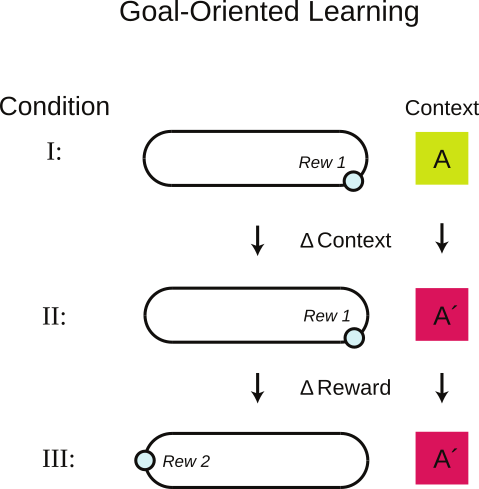
\includegraphics[width=0.5\textwidth]{df/Fig1_GOL}
	\caption[The three conditions of the GOL task]{Mice spend 3 days in each condition. \A/ and \Aprime/ are composed of different auditory, visual, olfactory, and tactile cues (see \nameref{sec:df:methods:contexts}), varied between Condition~I and Condition~II. The hidden reward location (blue circles, Rew~1 and Rew~2) is switched between Condition~II and Condition~III.}
	\label{fig:df:GOL}
\end{figure}
For this, we first trained water-deprived mice to run on a linear treadmill \citep{Danielson2016a, Danielson2016b, Royer2012} and then on the first day of the experiment introduced the mice to a novel environmental context, consisting of a feature-rich fabric belt and specific background non-spatial odor, tones, and blinking light patterns (\autoref{fig:df:contexts}).
\begin{figure}
	\centering
	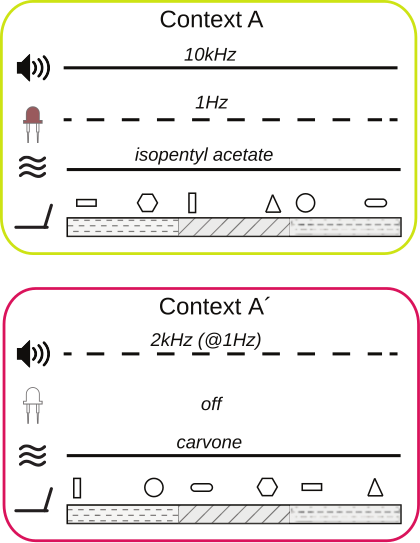
\includegraphics[width=0.5\textwidth]{df/Fig1_contexts}
	\caption[Components of the two distinct contexts used in the GOL task]{\A/ and \Aprime/ are composed of different auditory, visual, olfactory, and tactile cues (see Methods)}
	\label{fig:df:contexts}
\end{figure}
Operant water rewards were available at a single unmarked location on the belt; if the mouse licked in the correct location they received a water reward, but no water was administered if they did not lick in the reward location or if they licked outside the reward location (Condition~I, 3~days, 3~sessions per day).  We recorded the time of each lick as well as the position of the mouse on the treadmill in order to both determine when to deliver water rewards and to provide a readout of learning. As the mice learned the reward location they switched from exploratory licking along the entire belt, to focused licking only at the reward location, suppressing licking at other locations (\autoref{fig:df:licktograms}).
\todo[color=green]{horizontal licktograms}
\begin{figure}
	\centering
	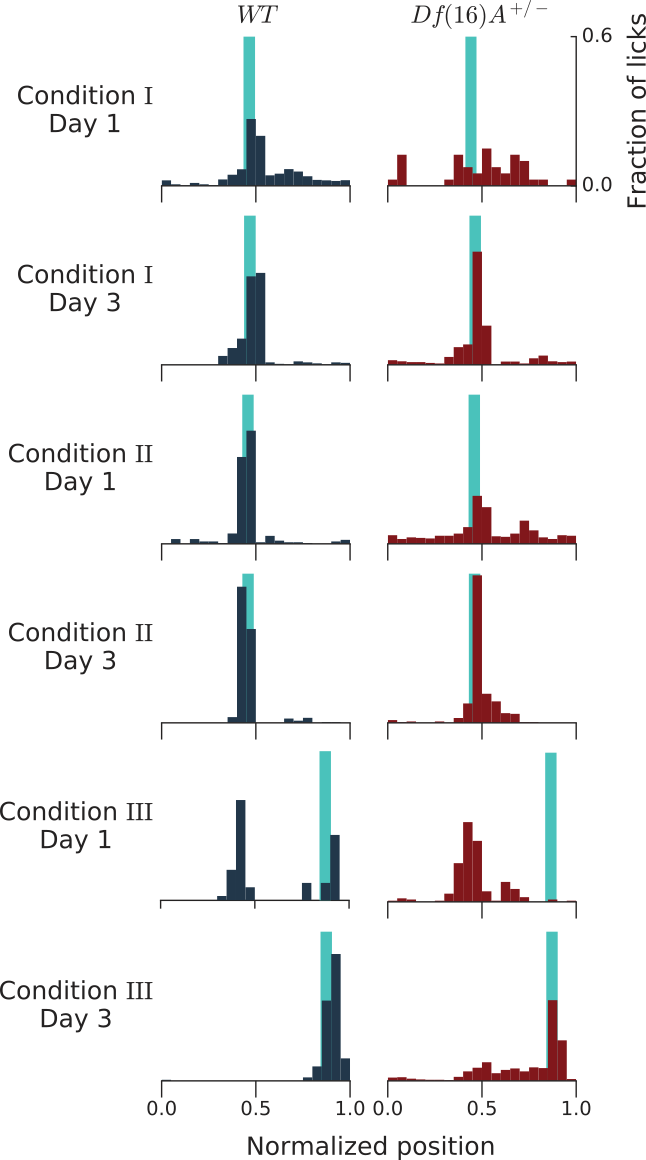
\includegraphics[width=0.5\textwidth]{df/Fig1_licktograms}
	\caption[Example histograms of lick counts by position]{Example histograms of lick counts by position for a WT (blue) and a \df/ (red) mouse on the first and last day of each condition. Cyan bars depict reward locations. As learning progresses, licking becomes increasingly specific for the reward location.}
	\label{fig:df:licktograms}
\end{figure}
In order to test the ability of mice to adjust to changes in the task conditions, we challenged mice by exposing them to an altered context (same sequence of belt materials, shuffled local cues, different non-spatial odor, tone, and light, see \nameref{sec:df:methods:contexts}), while maintaining the same reward location relative to the belt fabric sequence (Condition~II, 3~days, 3~sessions per day). During the last part of the task, we changed the location of the hidden reward while maintaining the familiar context from Condition~II (Condition~III, 3~days, 3~sessions per day). As a point of clarity, we use the term `context' to refer to the entire environment and set of features present during the experiment, including the fabric belts, local cues, non-spatial odor, tone, and light, the head-fix apparatus and the microscope itself, but importantly not the un-cued reward location. Also, `position' is always in reference to the sequence of three distinct belt fabrics, which were always in the same order throughout all Conditions of the experiment.

\subsection{\df/ mice are impaired in GOL task following changes in both context and reward location}
\label{sec:df:results:task_performance}
Our overall behavioral analysis on the GOL task revealed general differences among genotypes (Two-way RM ANOVA all days and Conditions, main effect of Genotype: p=0.004; main effect of Condition: n.s.), which developed in a condition dependent manner (Two-way RM ANOVA, Condition $\times$ Genotype interaction: p=0.036). In more detail, we found that both \df/ mice and wild-type (WT) littermates had a similar ability to learn the initial location of the hidden reward, as assessed by the suppression of un-rewarded licks outside of the reward zone and an increase in the fraction of licks within the reward zone (Condition~I, two-way RM ANOVA, main effect of Day: p$<$0.0001; Genotype $\times$ Day interaction and main effect of Genotype: n.s.; Figures \ref{fig:df:licktograms}, \ref{fig:df:task_performance}).
\begin{figure}
	\centering
	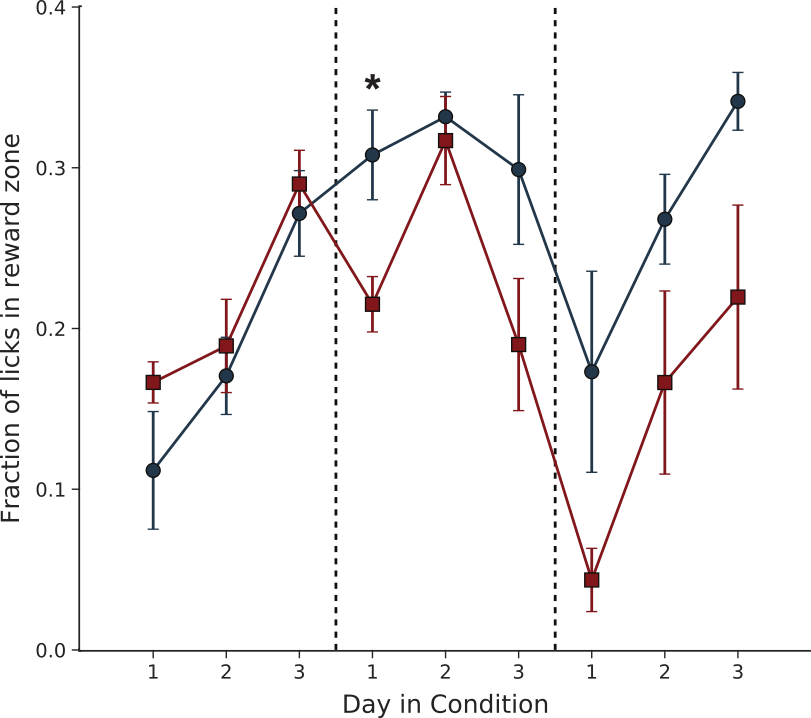
\includegraphics[width=0.7\textwidth]{df/Fig1_task_performance}
	\caption[Learning performance of WT and \df/ mice based on fraction of licks in the reward zone]{Learning performance of WT and \df/ mice based on fraction of licks in the reward zone (Two-way RM ANOVA, all days and Conditions, n=6 mice per genotype, main effect of Genotype: F(1,10)=13.634, p=0.004; Genotype $\times$ Condition interaction: F(2,40)=3.946, p=0.036; main effect of Condition: n.s.) for each day and Condition (Condition~I, two-way RM ANOVA, main effect of Day: F(2,20)=28.235, p$<$0.0001; Condition~II, two-way RM ANOVA, main effect of Genotype: F(1,10)=6.297, p=0.031; main effect of Day: F(2,20)=4.076, p=0.033; Condition~II post-hoc for individual days with Bonferroni correction, day 1: p=0.015; Condition~III, two-way RM ANOVA, main effects of Day: F(2,20)=15.762, p$<$0.0001; main effect of Genotype: F(1,10)=7.768, p=0.019; effects not listed: n.s.).  *p$<$0.05}
	\label{fig:df:task_performance}
\end{figure}
During this initial learning period, both WT and \df/ mice explored the task at similar levels (velocity, lap rate, lick rate, \autoref{fig:df:behavior_compare}). A change in the environmental context (Condition~II) had no detectable effect on WT animals, as their learning of the reward location in the new context continued to improve until their performance plateaued. However, this contextual manipulation impacted learning in the \df/ mice, as their task performance dropped on the first day and was overall worse than WT mice during Condition~II (Condition~II, two-way RM ANOVA, main effect of Genotype: p=0.031; main effect of Day: p=0.033; Genotype $\times$ Day interaction: n.s.; Figures \ref{fig:df:licktograms}, \ref{fig:df:task_performance}). Moreover, changing the reward location while maintaining a familiar context (Condition~III) challenged \df/ mice to a greater degree than WT animals, as they were significantly impaired in acquiring the new reward location (Condition~III, two-way RM ANOVA, main effect of Day: p$<$0.0001; main effect of Genotype: p=0.019; Genotype $\times$ Day interaction: n.s.; Figures \ref{fig:df:licktograms}, \ref{fig:df:task_performance}). Overall locomotor and licking performance was not different between the two groups (laps per session: p=0.770; lick rate: p=0.686; \autoref{fig:df:laps_licks}e,f). Thus, although \df/ mice are initially able to perform a spatially-guided reward task, learning deficits are revealed by manipulation of task parameters, specifically the environmental context or the reward location.
\begin{figure}
	\centering
	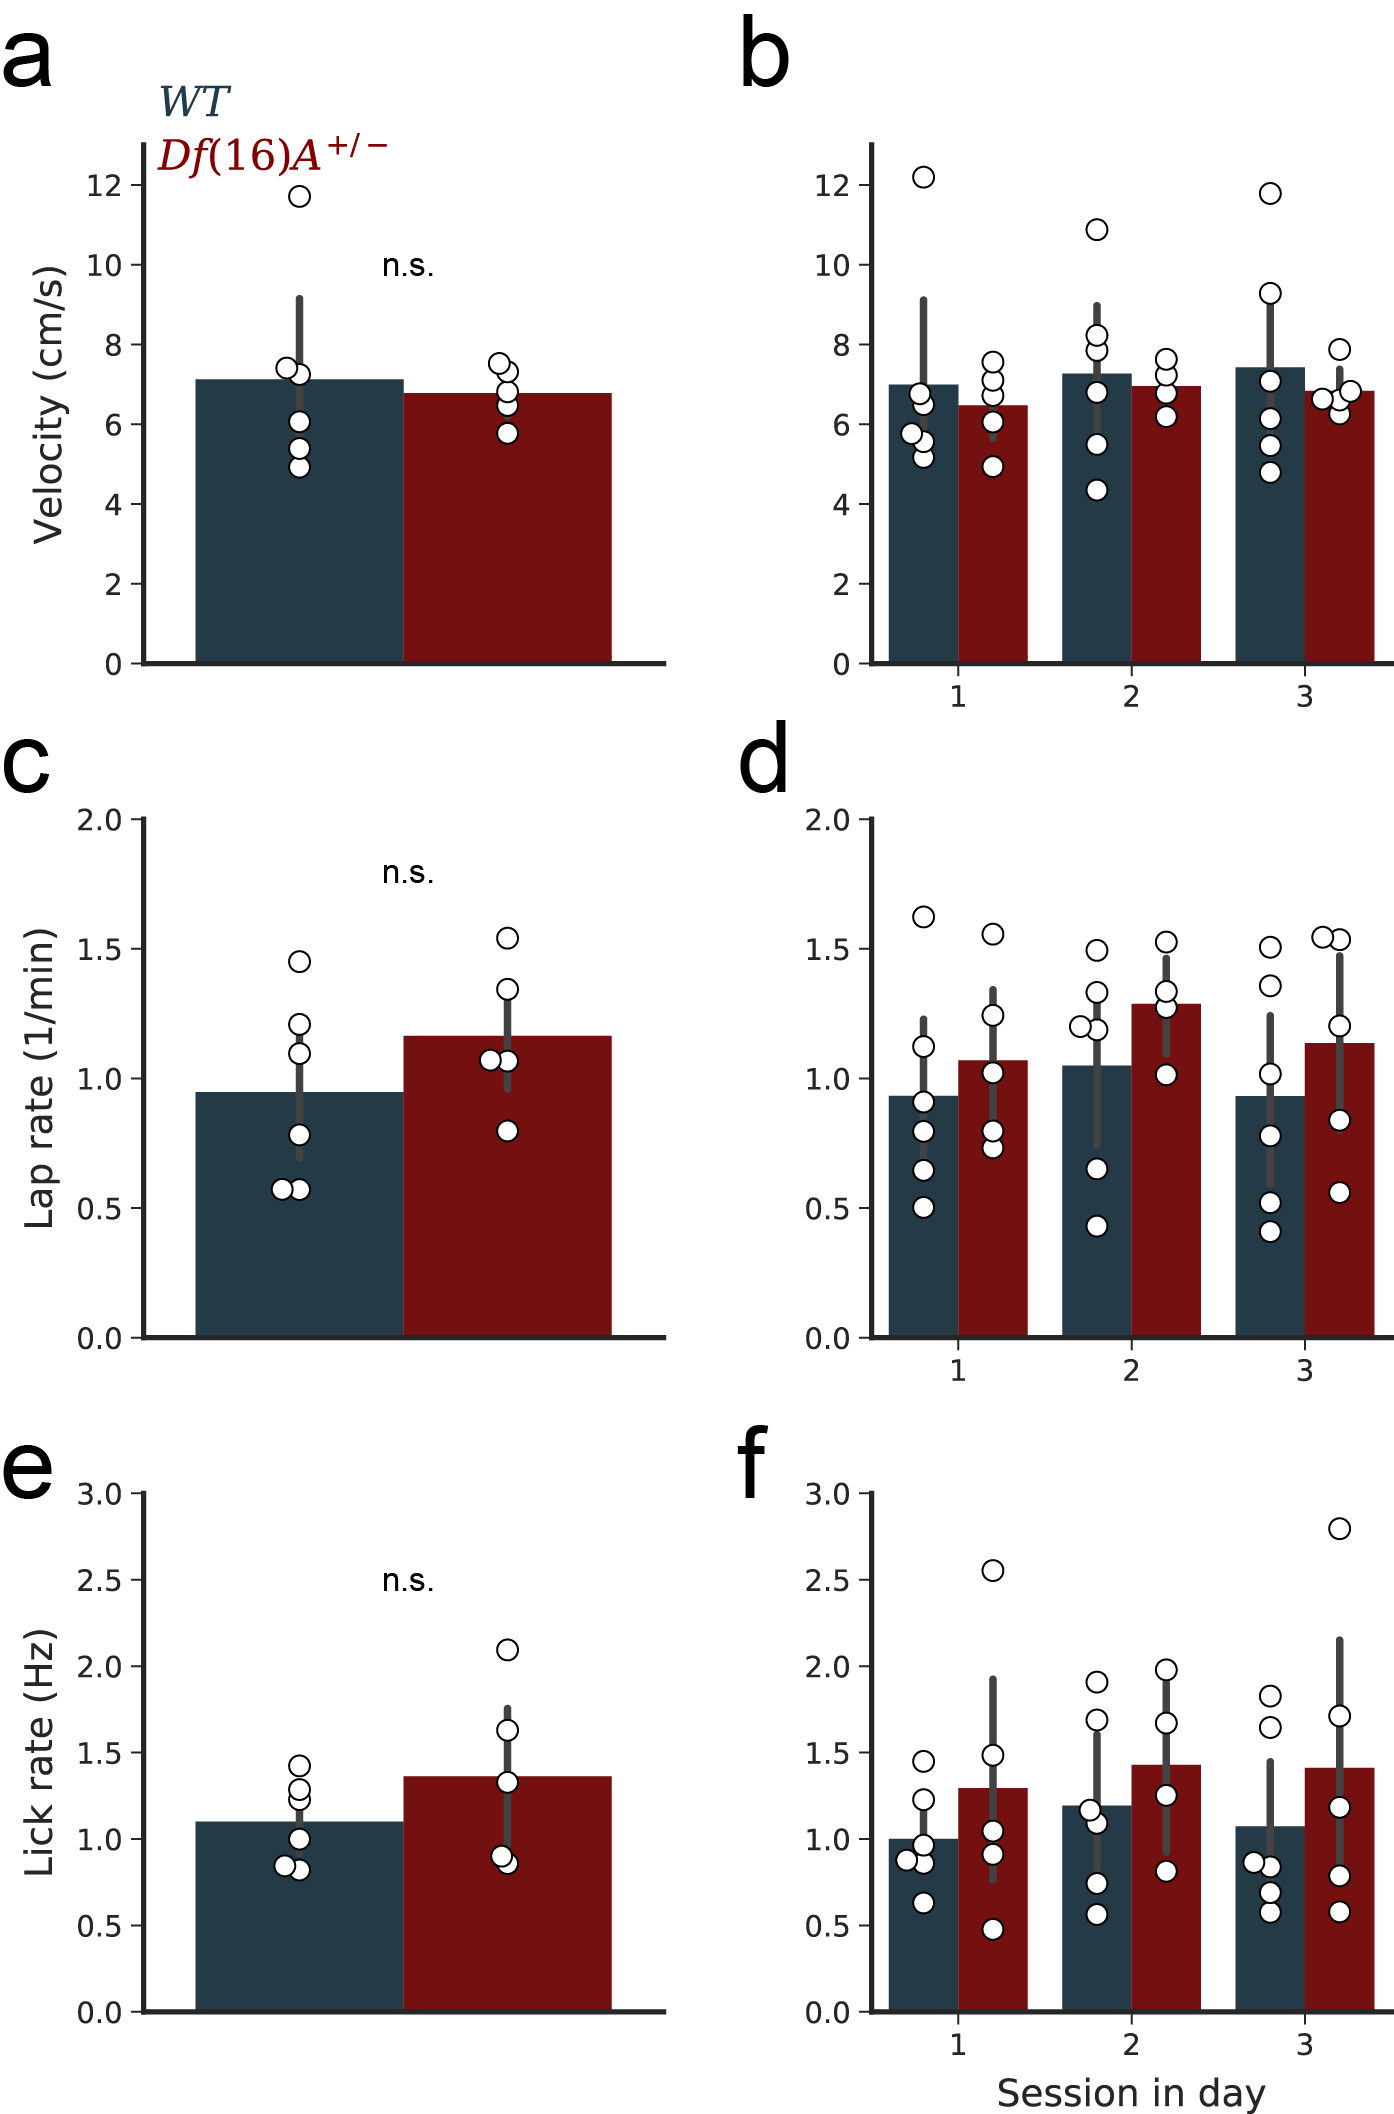
\includegraphics[width=0.5\textwidth]{df/FigS1_behavior_compare}
	\caption[Comparison of behavior during initial learning in GOL]{a. Mean velocity (excluding stationary time) during Condition~I for WT and \df/ mice. (WT: 7.123~$\pm$~1.002, n=6 mice; \df/: 6.778~$\pm$~0.312, n=5 mice; independent samples T-test, t=0.302, p=0.769). b. Velocity during Condition~I separated by session within each day (two-way ANOVA for session and genotype, all n.s.). c,d. Lap rate (as in a,b) (WT: 0.947~$\pm$~0.147, n=6 mice; \df/: 1.164~$\pm$~0.128, n=5 mice; independent samples T-test, t=-1.087, p=0.305; two-way ANOVA for session and genotype, all n.s.). e,f. Lick rate (as in a,b) (WT: 1.100~$\pm$~0.101, n=6 mice; \df/: 1.362~$\pm$~0.312, n=5 mice; independent samples T-test, t=-1.102, p=0.299; two-way ANOVA for session and genotype, all n.s.). Both WT and \df/ mice show similar levels of activity during the initial learning period, as well as across sessions within each day.}
	\label{fig:df:behavior_compare}
\end{figure}
\begin{figure}
	\centering
	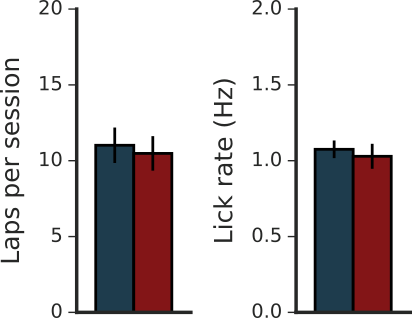
\includegraphics[width=0.5\textwidth]{df/Fig1_laps_licks}
	\caption[Laps and licks per session]{Left, Mean number of laps per session aggregated by mouse (WT: 11.018~$\pm$~1.279, n=6 mice, \df/: 10.482~$\pm$~1.246, n=6 mice, independent samples T-test: t=0.300, p=0.770).
	Right, Mean lick rate per mouse (WT: 1.075~$\pm$~0.064, n=6 mice, \df/: 1.029~$\pm$~0.090, n=6 mice, independent samples T-test: t=0.416, p=0.686).}
	\label{fig:df:laps_licks}
\end{figure}

We noticed during the task that \df/ mice appeared to be relatively more impaired at the start of each day, so to identify genotypic differences in the consolidation of the task memory overnight, we compared the task performance at the beginning and the end of the day during each condition (\autoref{fig:df:performance_by_session_in_day}).
\begin{figure}
	\centering
	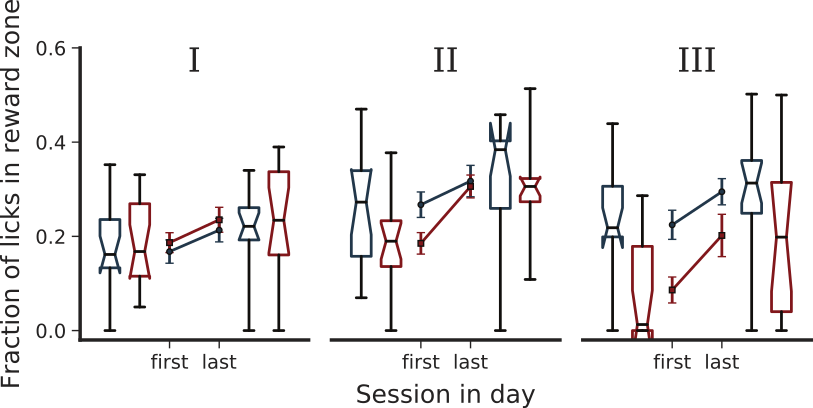
\includegraphics[width=0.7\textwidth]{df/Fig1_performance_by_session_in_day}
	\caption[Learning performance for WT and \df/ mice on the first and last session of each day]{Learning performance for WT and \df/ mice on the first and last session of each day by Condition. Across all conditions, both genotypes perform better at the end of the day. During Condition~I, WT and \df/ mice performs similarly throughout the day (two-way RM ANOVA, main effect of Session: F(1,10)=6.901, p=0.025; main effect of Genotype and Genotype $\times$ Session interaction: n.s.), while in Condition~II \df/ mice were more impaired at the start of the day (two-way RM ANOVA, main effect of Session: F(1,10)=40.506, p$<$0.0001; Genotype $\times$ Session interaction: F(1,10)=6.404, p=0.030; main effect of Genotype: n.s.), and in Condition~III they additionally never reached WT levels (two-way RM ANOVA, main effect of Genotype: F(1,10)=6.433, p=0.030; main effect of Session: F(1,10)= 53.237, p$<$0.0001; Genotype $\times$ Session interaction: n.s.).}
	\label{fig:df:performance_by_session_in_day}
\end{figure}
During Condition~I -- in which we observed no learning deficit in the \df/ mice -- both WT and \df/ mice performed at comparable levels throughout the day, and both performed better at the end of the day than at the beginning (Condition~I, two-way RM ANOVA, main effect of Session: p=0.025; main effect of Genotype and Genotype $\times$ Session interaction: n.s.). During Condition~II -- in which we observed an overall decrease in task performance in the \df/ mice --  we found that the \df/ animals performed poorly on the first session of each day, before reaching WT performance levels by the end of the day (Condition~II, two-way RM ANOVA, main effect of Session: p$<$0.0001; Genotype $\times$ Session interaction: p=0.030; main effect of Genotype: n.s.). Finally, during Condition~III -- in which we observed the most robust learning deficit in the \df/ mice -- we found that \df/ mice performed significantly worse throughout the entire day (Condition~III, two-way RM ANOVA, main effect of Genotype: p=0.030; main effect of Session: p$<$0.0001, Genotype $\times$ Session interaction: n.s.). Collectively, these results indicate that deficits in overnight consolidation likely contributed to the differences we observed between genotypes.

\subsection{Smaller, less diffuse place cell population in \df/ compared to WT mice}

We used two-photon Ca\super{2+} imaging of large neuronal populations in the CA1 pyramidal layer during the GOL task to assess basic coding properties of place cells (\autoref{fig:df:imaging_intro}). Spatially-tuned Ca\super{2+} transients \citep{Dombeck2007} (\autoref{fig:df:place_cells}) were detected in both WT and \df/, mice however we found that the fraction of identified neurons that exhibited place cell place cell properties was about 25\% less in \df/ mice compared to WT mice across all sessions (place cell fraction: WT: 0.2553~$\pm$~0.0109; \df/: 0.1924~$\pm$~0.0079; p$<$0.0001; \autoref{fig:df:place_metrics}a).  This effect is not driven by a silent fraction of cells in the \df/ mice or differences in our sampling of the pyramidal cells between the genotypes, as cumulatively over all imaging sessions the available place cell population was similar (lifetime place coding: p=0.244; \autoref{fig:df:supp_place_metrics}a). Instead, we see that individual cells were identified as place cells in fewer sessions (fraction of sessions a place cell: p$<$0.0001; \autoref{fig:df:supp_place_metrics}b). Furthermore, the spatial tuning of individual place cells in \df/ mice was less diffuse, as indicated by differences in the number of place fields per place cell (place fields per place cell: p$<$0.0001; \autoref{fig:df:place_metrics}b), slightly narrower place fields (place field width: p$<$0.0001; Figures \ref{fig:df:place_metrics}c, \autoref{fig:df:supp_place_metrics}e), less variability in Ca\super{2+} transient firing location (circular variance; p$<$0.0001; inset averaged by mouse, p=0.0491; \autoref{fig:df:place_metrics}d), and less out-of-field firing (transient specificity: p$<$0.0001; \autoref{fig:df:supp_place_metrics}d).
\todo[color=cyan]{Here you can add the part from the rebuttal, including the Kentros, Hussaini and Fenton, Kjestrup}
Overall, the significant decrease in the fraction of spatially-tuned cells and altered firing field properties suggests a disruption in the processing of spatial information in the pathological hippocampal network of \df/ mice.

\begin{figure}
	\centering
	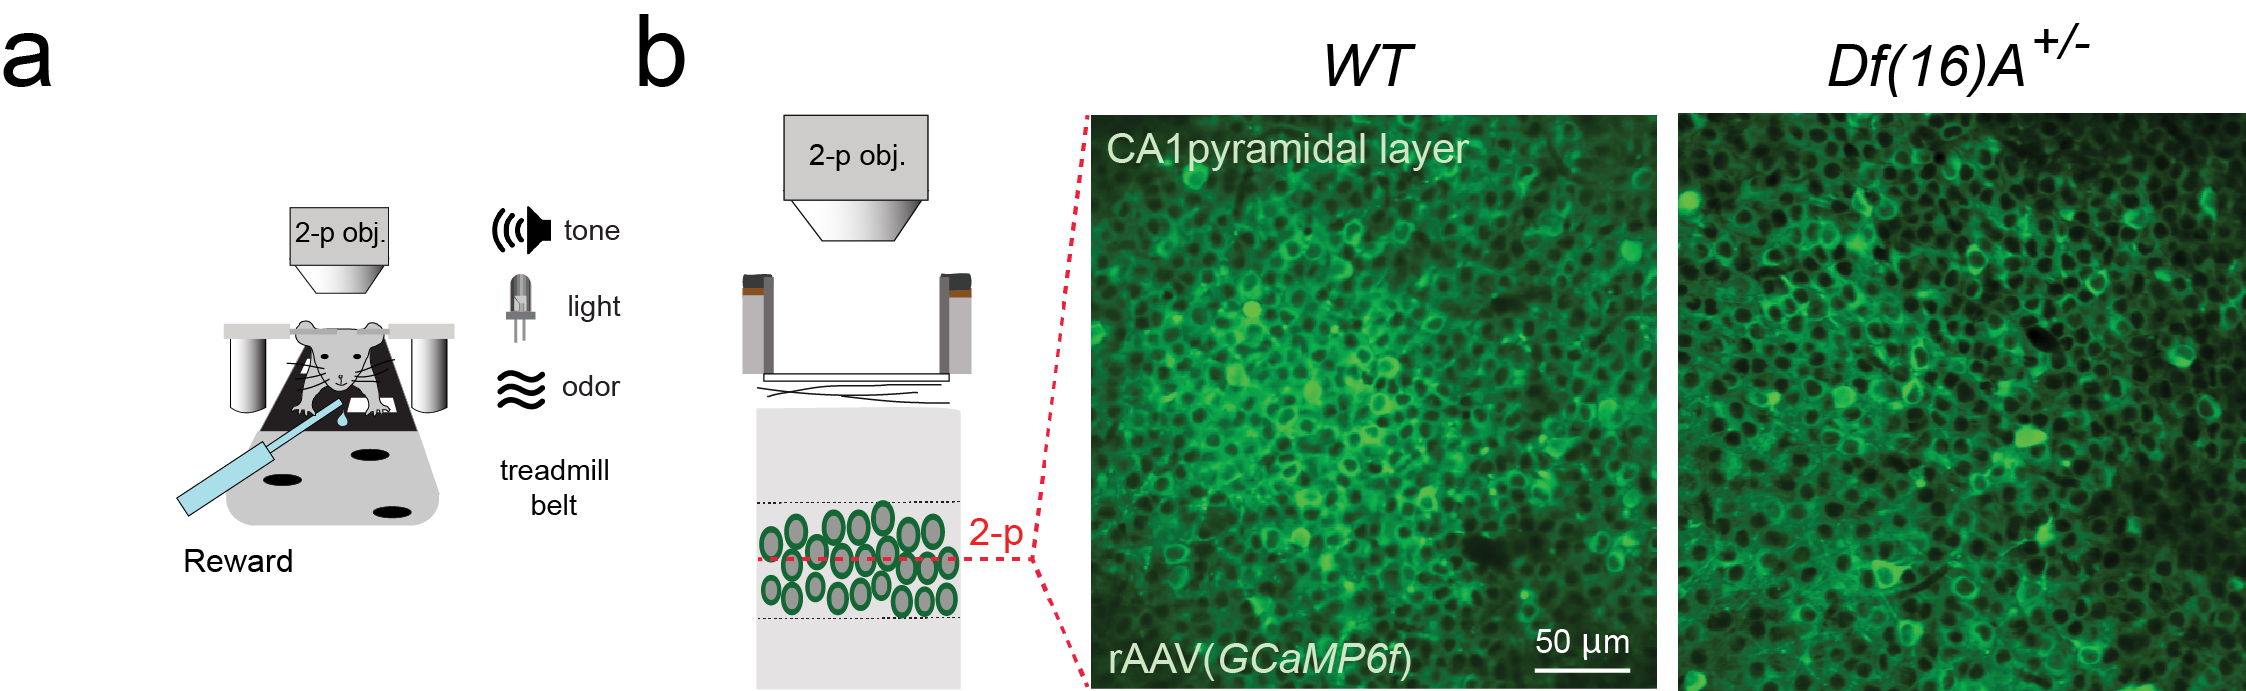
\includegraphics[width=0.9\textwidth]{df/Fig2_imaging_intro}
	\caption[Schematic of head-fixed setup and example fields of view]{a. Schematic of head-fixed behavioral setup.
	b. Left: schematic of two-photon Ca\super{2+} imaging in the CA1 pyramidal layer. Representative two-photon fields of view across the pyramidal layer showing cross-sections of GCaMP6f-expressing cell bodies from a WT (middle) and \df/ (right) mouse. 179-621 regions of interest (ROIs, see \autoref{sec:df:methods:surgery}) corresponding to cell bodies were imaged chronically in each field of view.}
	\label{fig:df:imaging_intro}
\end{figure}

\begin{figure}
	\centering
	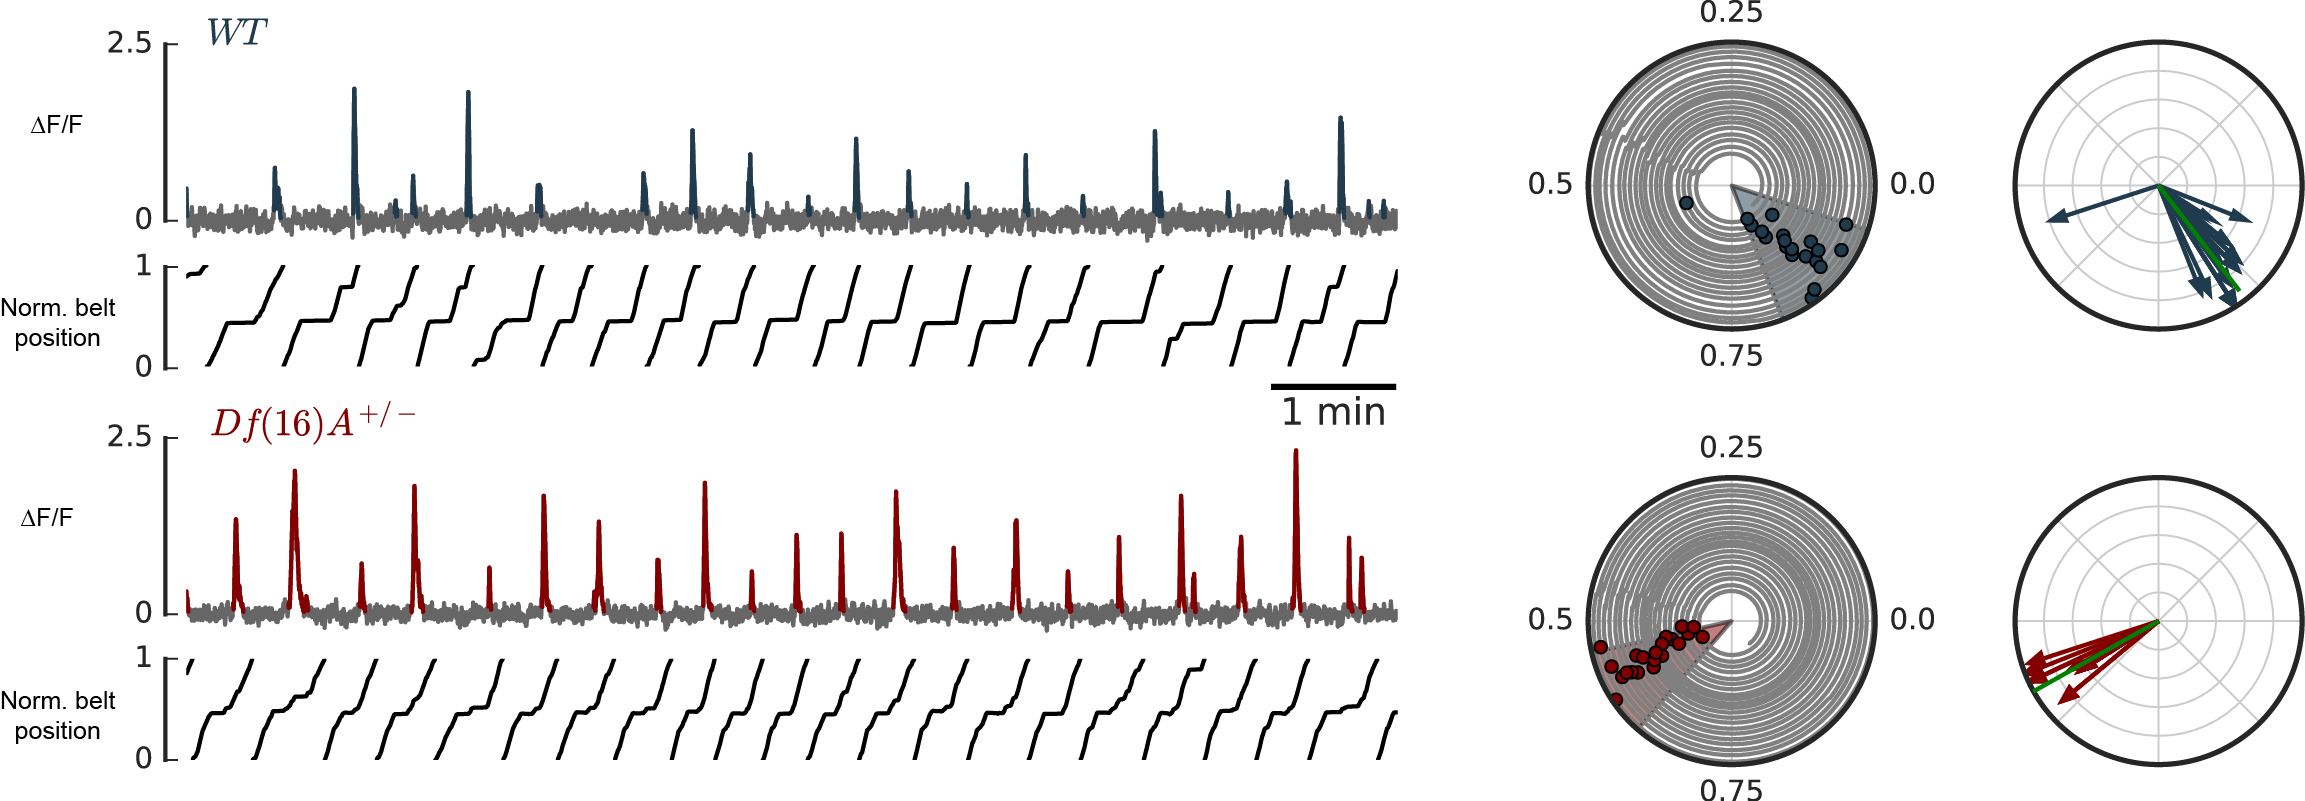
\includegraphics[width=0.9\textwidth]{df/Fig2_place_cells}
	\caption[Example Ca\super{2+} traces and spatial tuning]{Left, GCaMP6f Ca\super{2+} fluorescence ($\Delta F/F$) traces from two example spatially-tuned CA1 place cells in WT and \df/ mice during 10 minute sessions. Significant Ca\super{2+} transients are highlighted in blue/red, and treadmill position is shown below the traces.
	Middle, polar trajectory plots showing significant running-related transients for the same example cells. The animals' position (angle) over time (radius) is grey, the onset times of significant running-related calcium transients are shown as colored circles. Shaded areas denote place fields. 
	Right, transient vector plots showing the position (angle) and occupancy-normalized weight of each running-related transient (radius), as used to calculate occupancy-normalized transient rate histograms and transient circular variance. Green lines indicate transient resultant vector (the magnitude is $1 – circular variance$).}
	\label{fig:df:place_cells}
\end{figure}

\begin{figure}
	\centering
	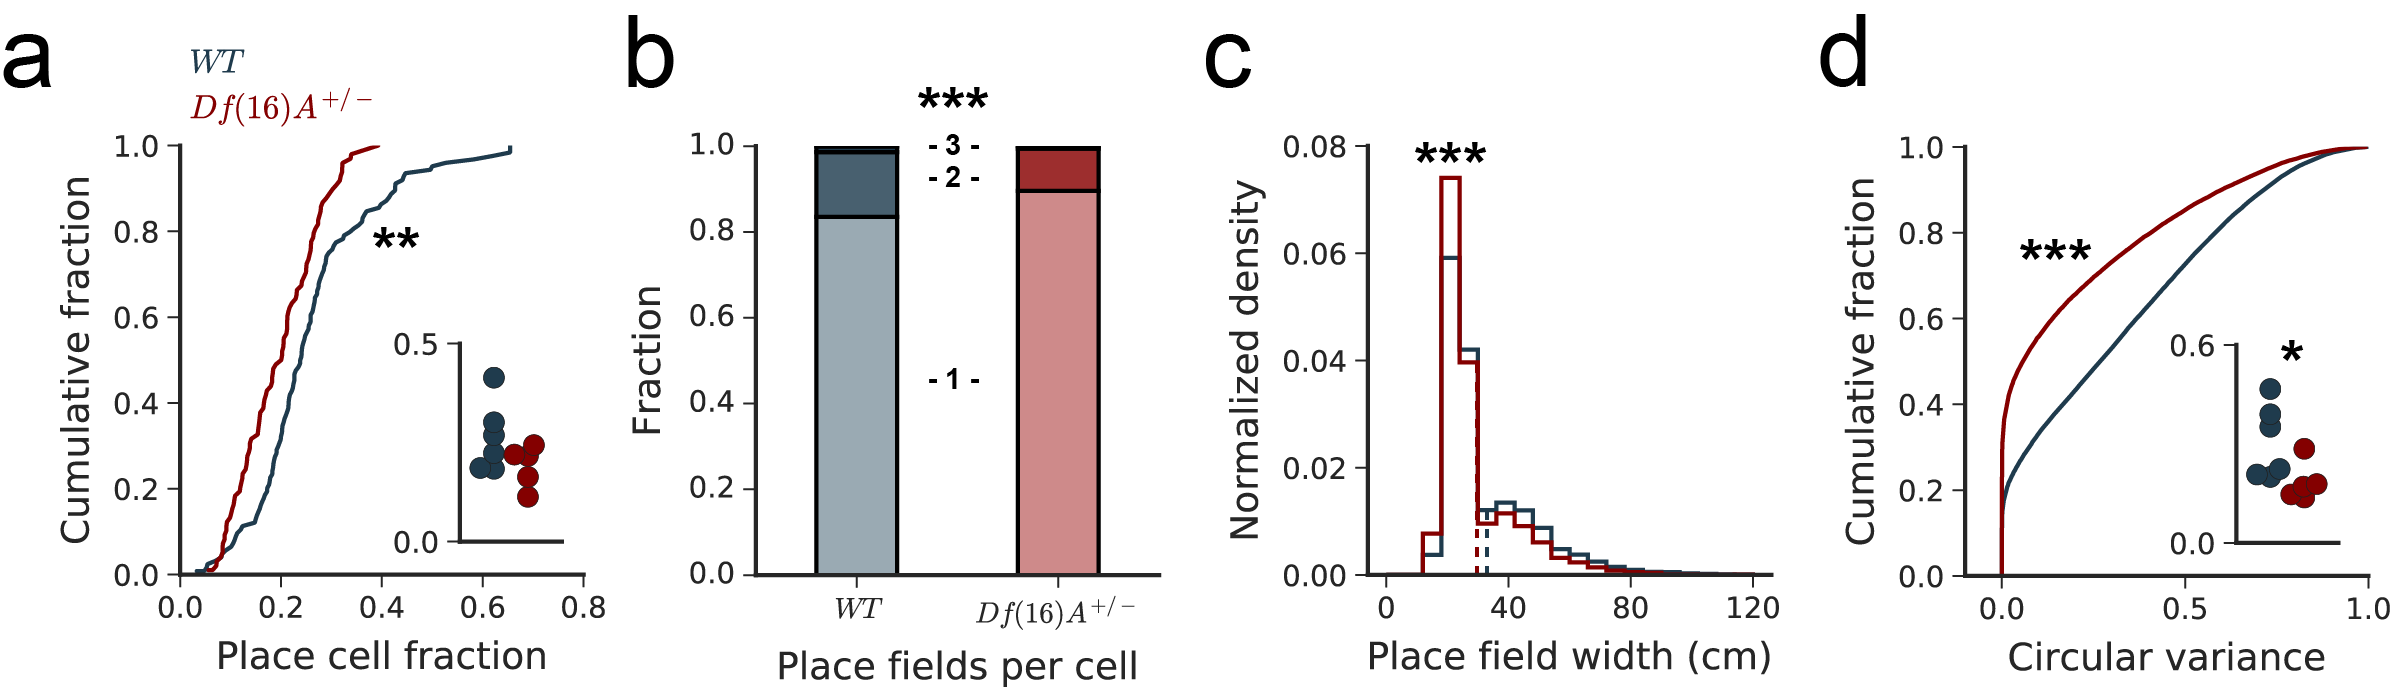
\includegraphics[width=0.9\textwidth]{df/Fig2_place_metrics}
	\caption[Comparison of place cell metrics]{Compared to WT, \df/ mice had a decreased fraction of cells per experiment with significant spatial information (place cell fraction: WT: 0.2553~$\pm$~0.0109, n=124 sessions; \df/: 0.1924~$\pm$~0.0079, n=98 sessions; Mann-Whitney U, U=4214.5, p$<$0.0001; inset averaged by mouse, independent samples T-test, t=1.620, p=0.140; a), fewer multi-peaked place cells (place fields per place cell; WT: 1.180~$\pm$~0.004, n=12571 PC*sessions; \df/: 1.110~$\pm$~0.004, n=7683 PC*sessions; Pearson chi-square test: $\chi^2$=228.650, p$<$0.0001; Mann-Whitney U, U=$4.53\times10^7$, p$<$0.0001; e), narrower place fields (place field width; WT: 32.531~$\pm$~0.135, n=12571 PC*sessions; \df/: 29.532~$\pm$~0.144, n=7683 PC*sessions; Mann-Whitney U, U=$4.123\times10^7$, p$<$0.0001; f), and lower circular variance (WT: 0.310~$\pm$~0.0013, n=43068 cell*sessions; \df/: 0.189~$\pm$~0.0014, n=27397 cell*sessions, Mann-Whitney U, U=$4.21\times10^8$, p$<$0.0001; inset averaged by mouse, Welch's T-test, t=2.327, p=0.0491, g). *p$<$0.05, **p$<$0.01, ***p$<$0.001}
	\label{fig:df:place_metrics}
\end{figure}

\begin{figure}
	\centering
	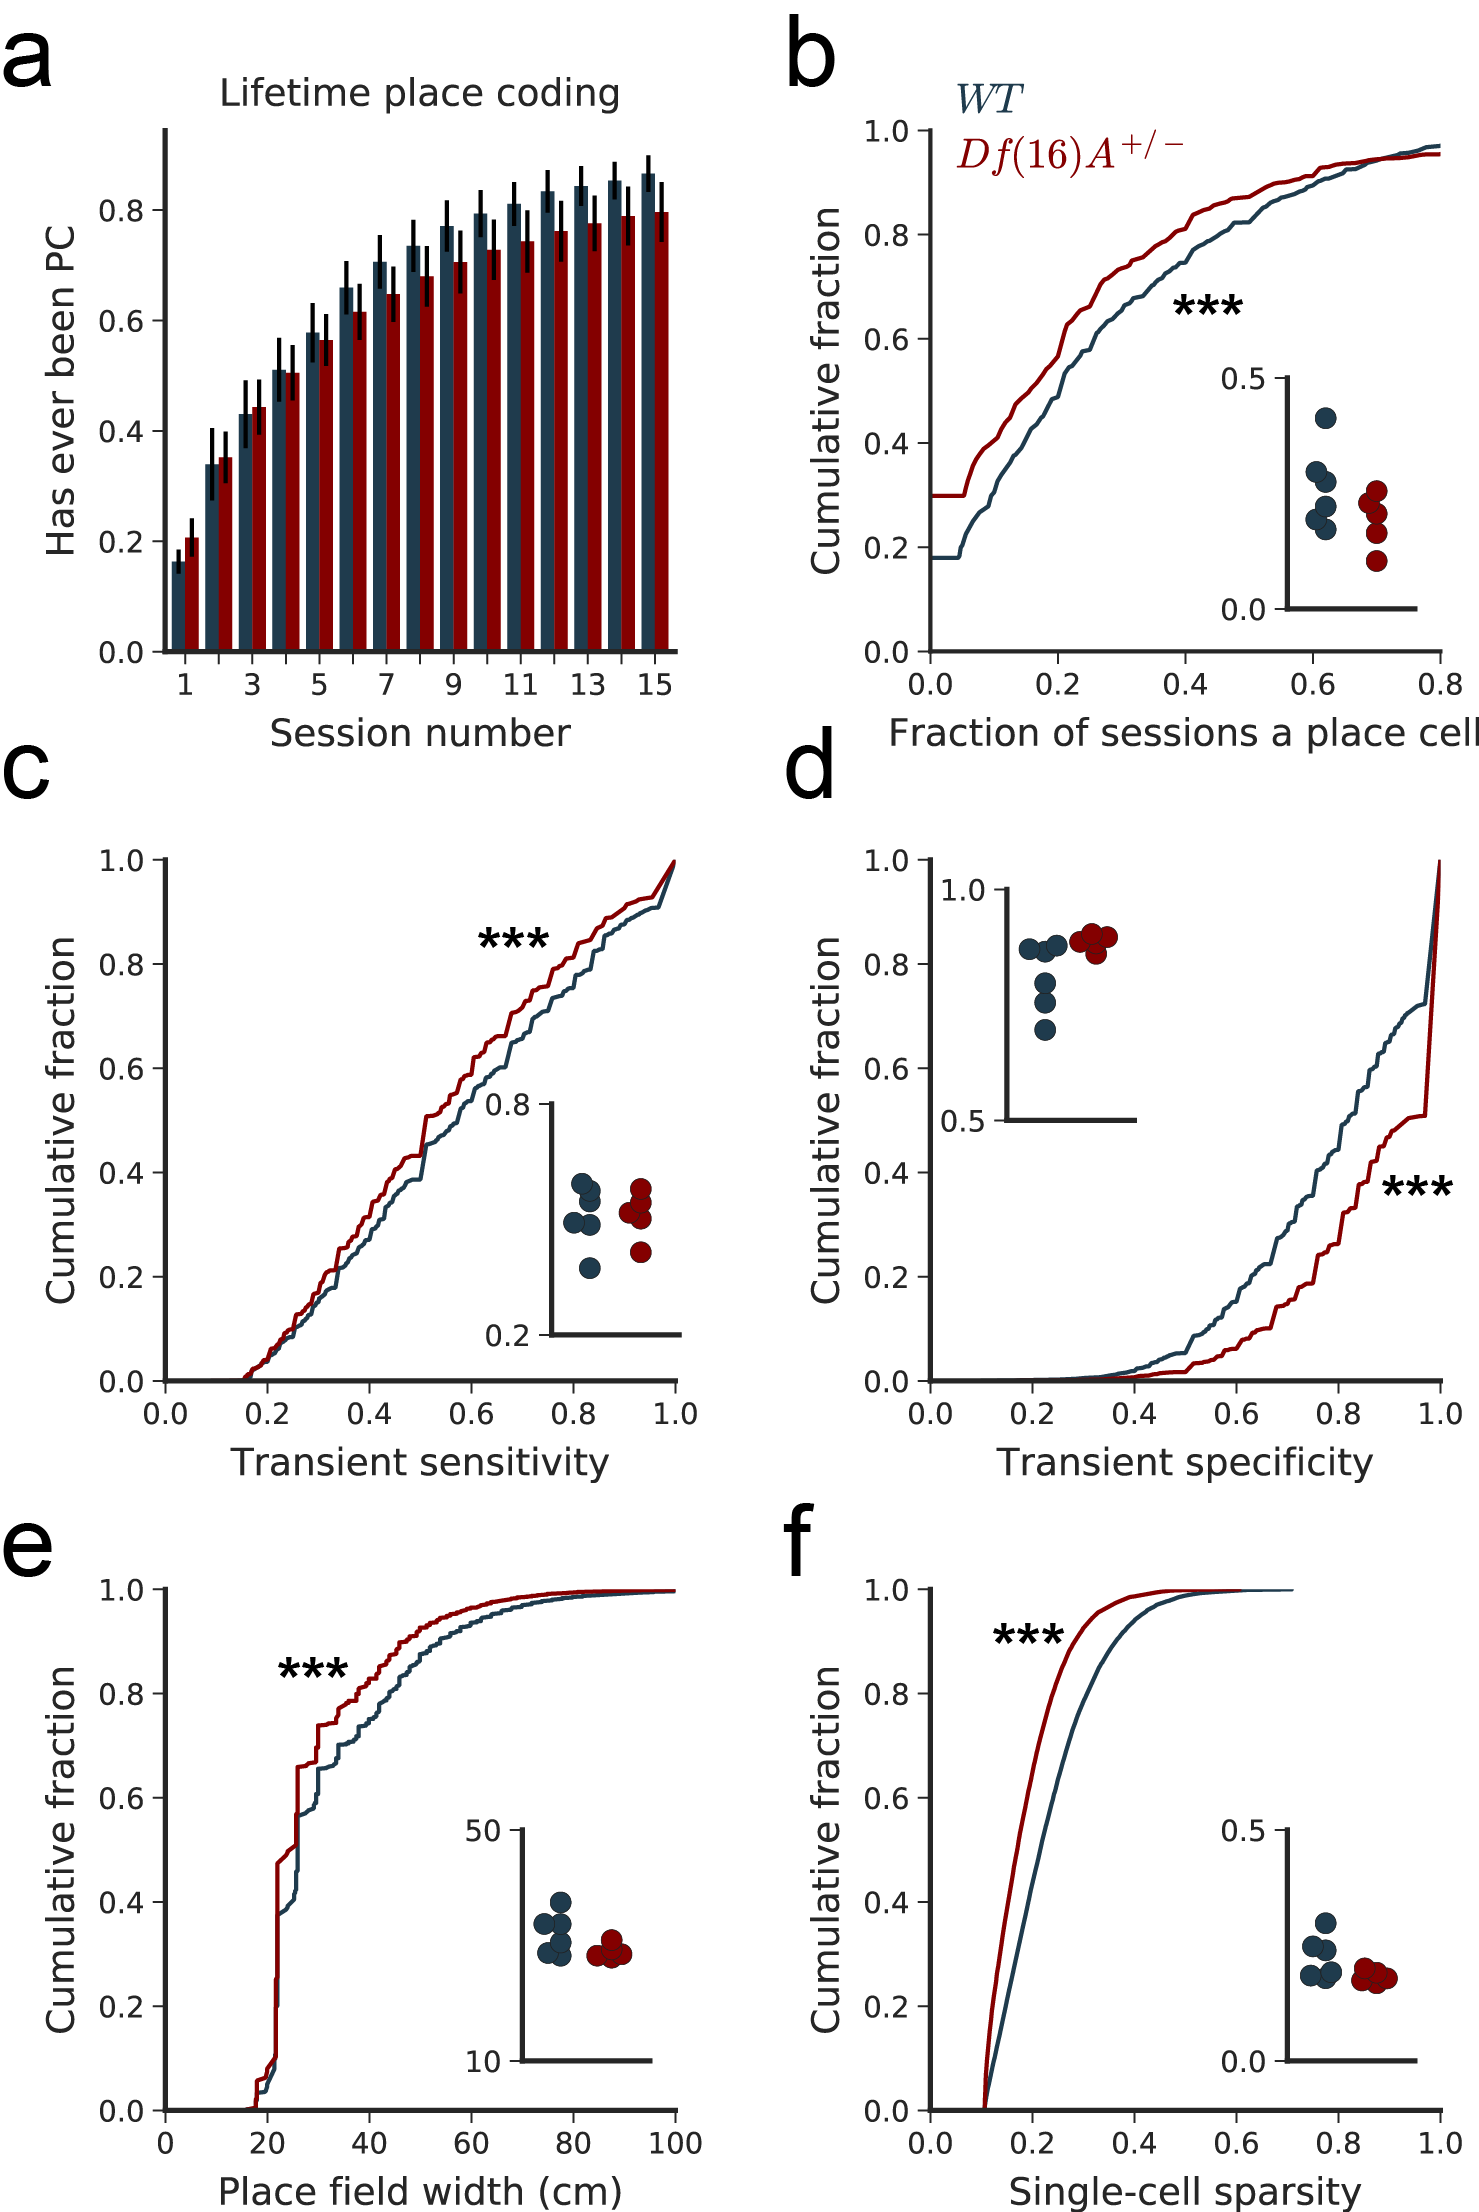
\includegraphics[width=0.6\textwidth]{df/FigS2_place_cell_metrics}
	\caption[Comparison of lifetime place coding and additional place cell metrics]{a. Lifetime place coding percentage, the fraction of ROIs that were ever identified as a place cell by the nth session imaged (lifetime place coding, Cox Regression, B=0.222, p=0.244).
	b. Fraction of all sessions imaged that an ROI was identified as a place cell (fraction of sessions a place cell; WT: 0.254~$\pm$~0.004, n=3162 cells; \df/: 0.214~$\pm$~0.004, n=3322 cells; Mann-Whitney U, U=$4.55\times10^6$, p$<$0.0001), averaged within mice (inset; independent sample T-test, t=1.517, p=0.164).
	c. Transient sensitivity, defined as the fraction of laps in which a transient occurred in the place field (WT: 0.5786~$\pm$~0.00218, n=12524 place cell*sessions; \df/: 0.5445~$\pm$~0.0027, n=7664 place cell*sessions; Mann-Whitney U, U=$4.4\times10^7$, p$<$0.0001), averaged within mice (inset, independent samples T-test, t=0.0142, p=0.989).
	d. Transient specificity, defined as the fraction of transients that occurred in the place field (WT: 0.795~$\pm$~0.0161, n=12571 place cell*sessions; \df/: 0.872~$\pm$~0.0018, n=7683 place cell*sessions; Mann-Whitney U, U=$3.59\times10^7$, p$<$0.0001), averaged within mice (inset; Welch's T-test, t=2.427, p=0.0544).
	e. Place field width (WT: 32.09~$\pm$~0.125, n=14833 place fields; \df/: 29.25~$\pm$~0.136, n=8529 place fields; Mann-Whitney U, U=$5.5\times10^7$ p$<$0.0001), averaged within mice (inset, Welch's T-test, t=1.990, p=0.0911).
	f. Single-cell sparsity (WT: 0.2325~$\pm$~0.001, n=12571 ROI*sessions; \df/: 0.186~$\pm$~0.001, n=8683 ROI*sessions; Mann-Whitney U, U=$3.35\times10^7$, p$<$0.0001), averaged within mice (inset, Welch's T-test, t=2.064, p=0.0852). ***p$<$0.001}
	\label{fig:df:supp_place_metrics}
\end{figure}

\subsection{Spatial map is less stable in \df/ compared to WT mice}
\label{sec:df:results:stability}
To examine the evolution of spatial maps throughout the GOL task we repeatedly imaged the same populations of individually-identified neurons throughout the 27 sessions across 9 days during the GOL task (cells per mouse, mean~$\pm$~s.d.; WT: 463~$\pm$~37, n=6 mice; \df/: 479~$\pm$~84, n=5 mice), and looked at two aspects of stability: place cell population stability (recurrence probability: probability of a cell being identified as a place cell in paired sessions) and individual pyramidal cell firing stability (centroid shift: distance between centroid of firing in paired sessions). Combining all conditions and sessions, we found that individual place cells recurred \citep{Ziv2013} from day-to-day significantly above chance levels in WT and \df/ mice (recurrence probability: WT vs. shuffle: p=$<$0.0001; \df/ vs. shuffle: p$<$0.0001; \autoref{fig:df:recurrence}a), but a significantly smaller fraction of place cells re-occurred from day-to-day in \df/ than WT mice (WT vs. \df/: p$<$0.0001; inset by mouse, p=0.028; \autoref{fig:df:recurrence}a). This decreased overlap in place cell population in the \df/ mice primarily driven by decreased stability overnight, as this difference was not observed within day from session-to-session (two-way ANOVA; Genotype $\times$ Elapsed Time interaction: p=0.0118; post-hoc analysis, WT vs. \df/, S-S: p=0.325; D-D, p$<$0.0001; \autoref{fig:df:recurrence}b), again suggesting a disruption in overnight consolidation, as seen with the \df/ behavioral performance (see \autoref{fig:df:performance_by_session_in_day}).

\begin{figure}
	\centering
	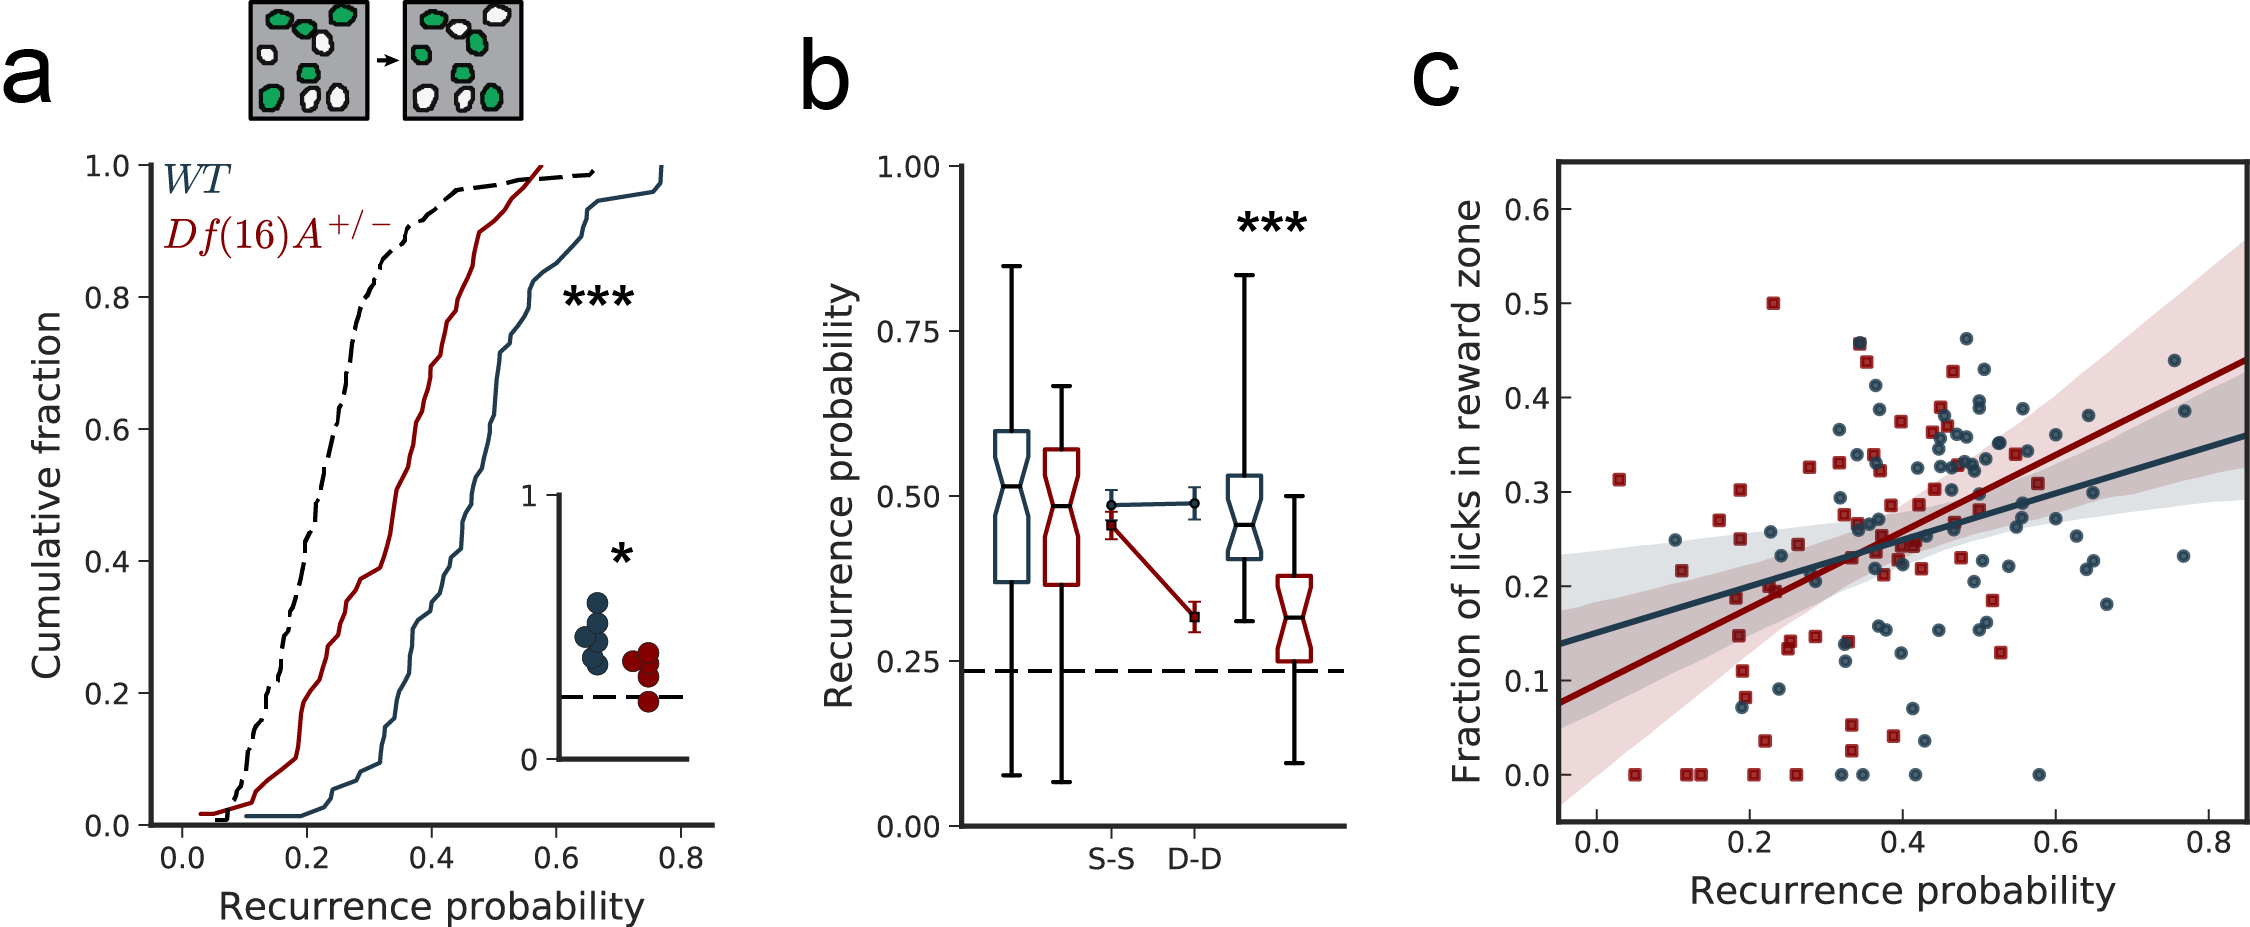
\includegraphics[width=0.8\textwidth]{df/Fig3_recurrence}
	\caption[Comparison of recurrence probability]{a. (top) Example of place cell recurrence. In a given field of view, a subset of all cells has significant spatial tuning each day (place cells, green). The overlap in this population is the recurrence probability (40\% in this example).
	(bottom) Distribution of recurrence fractions from day-to-day for WT and \df/ mice for all sessions (dotted line is cell-identity shuffle distribution: WT: 0.456~$\pm$~0.015, n=74 sessions, \df/: 0.327~$\pm$~0.017, n=59 sessions, shuffle: 0.229~$\pm$~0.009, n=133 sessions; WT vs. shuffle: Welch's T-test, t=12.64, p=$<$0.0001; \df/ vs. shuffle: Welch's T-test, t=5.124, p$<$0.0001; WT vs. \df/: independent samples T-test, t=5.72, p$<$0.0001) and aggregated by mouse (inset, gray bar is cell-identity shuffle: WT vs. \df/: independent samples T-test, t=2.611, p=0.028). b. Mean fraction of cells that reoccur as place cells from session-to-session (S-S) or day-to-day (D-D) for WT and \df/ mice (dotted line is mean place cell fraction; two-way ANOVA for elapsed time and genotype; main effect of Genotype: F(1,152)=8.199, p=0.0048; main effect of Time: F(1,152)=4.434, p=0.0369; Time $\times$ Genotype interaction: F(1,152)=6.493, p=0.0118; post-hoc analysis, WT vs. \df/, S-S: t=0.988, p=0.325; D-D: t=5.012, p$<$0.0001). c. Correlation of place cell recurrence with performance throughout the task. Solid line is linear regression fit, shaded regions are 95\% confidence intervals calculated from bootstrap resampling (Pearson's correlation coefficient, WT: 0.288, p=0.013; \df/: 0.416, p=0.001; WT correlation vs. \df/ correlation, Fisher Z transformation of correlations, GLM model, Univariate Analysis of Variance: Genotype $\times$ Recurrence interaction: F(1,132)=0.599, p=0.440). *p$<$0.05, ***p$<$0.001}
	\label{fig:df:recurrence}
\end{figure}

We next looked at the shift in firing locations in both WT and \df/ mice to assess the similarity of spatial tuning from day-to-day. We found that while preferred firing locations of all cells were more stable than chance in both genotypes (centroid shift: WT vs. shuffle: p$<$0.0001; \df/ vs. shuffle: p$<$0.0001; \autoref{fig:df:cent_shift}a; place field correlation: WT vs. shuffle: p$<$0.0001; \df/ vs. shuffle: p$<$0.0001; \autoref{fig:df:pf_corr}a), the spatial tuning in \df/ mice was significantly less stable day-to-day compared to WT mice (centroid shift: WT vs. \df/: p$<$0.0001; inset by mouse: p=0.030; \autoref{fig:df:cent_shift}a; place field correlation: WT vs. \df/: p$<$0.0001; \autoref{fig:df:pf_corr}a). Also, just as the active place cell population overlap was similar within day between WT and \df/ mice, spatial tuning was also not different between WT and \df/ mice from session-to-session within the same day (centroid shift: two-way ANOVA, Genotype $\times$ Elapsed Time interaction: p=0.0696; post-hoc analysis, WT vs. \df/, S-S: p=0.694; D-D, p=0.0047; \autoref{fig:df:cent_shift}b; place field correlation: Genotype $\times$ Elapsed Time interaction: p=0.0051; post-hoc analysis, WT vs. \df/, S-S: p=0.613; D-D, p$<$0.0001; \autoref{fig:df:pf_corr}b). Taken together, spatial maps are less stable in \df/ than WT mice from day-to-day (but not from session-to-session), as seen by lower recurrence of place cells and a larger shift in spatial tuning centroids, reflecting severely disrupted spatial maps in the \df/ mutant mice.

\begin{figure}
	\centering
	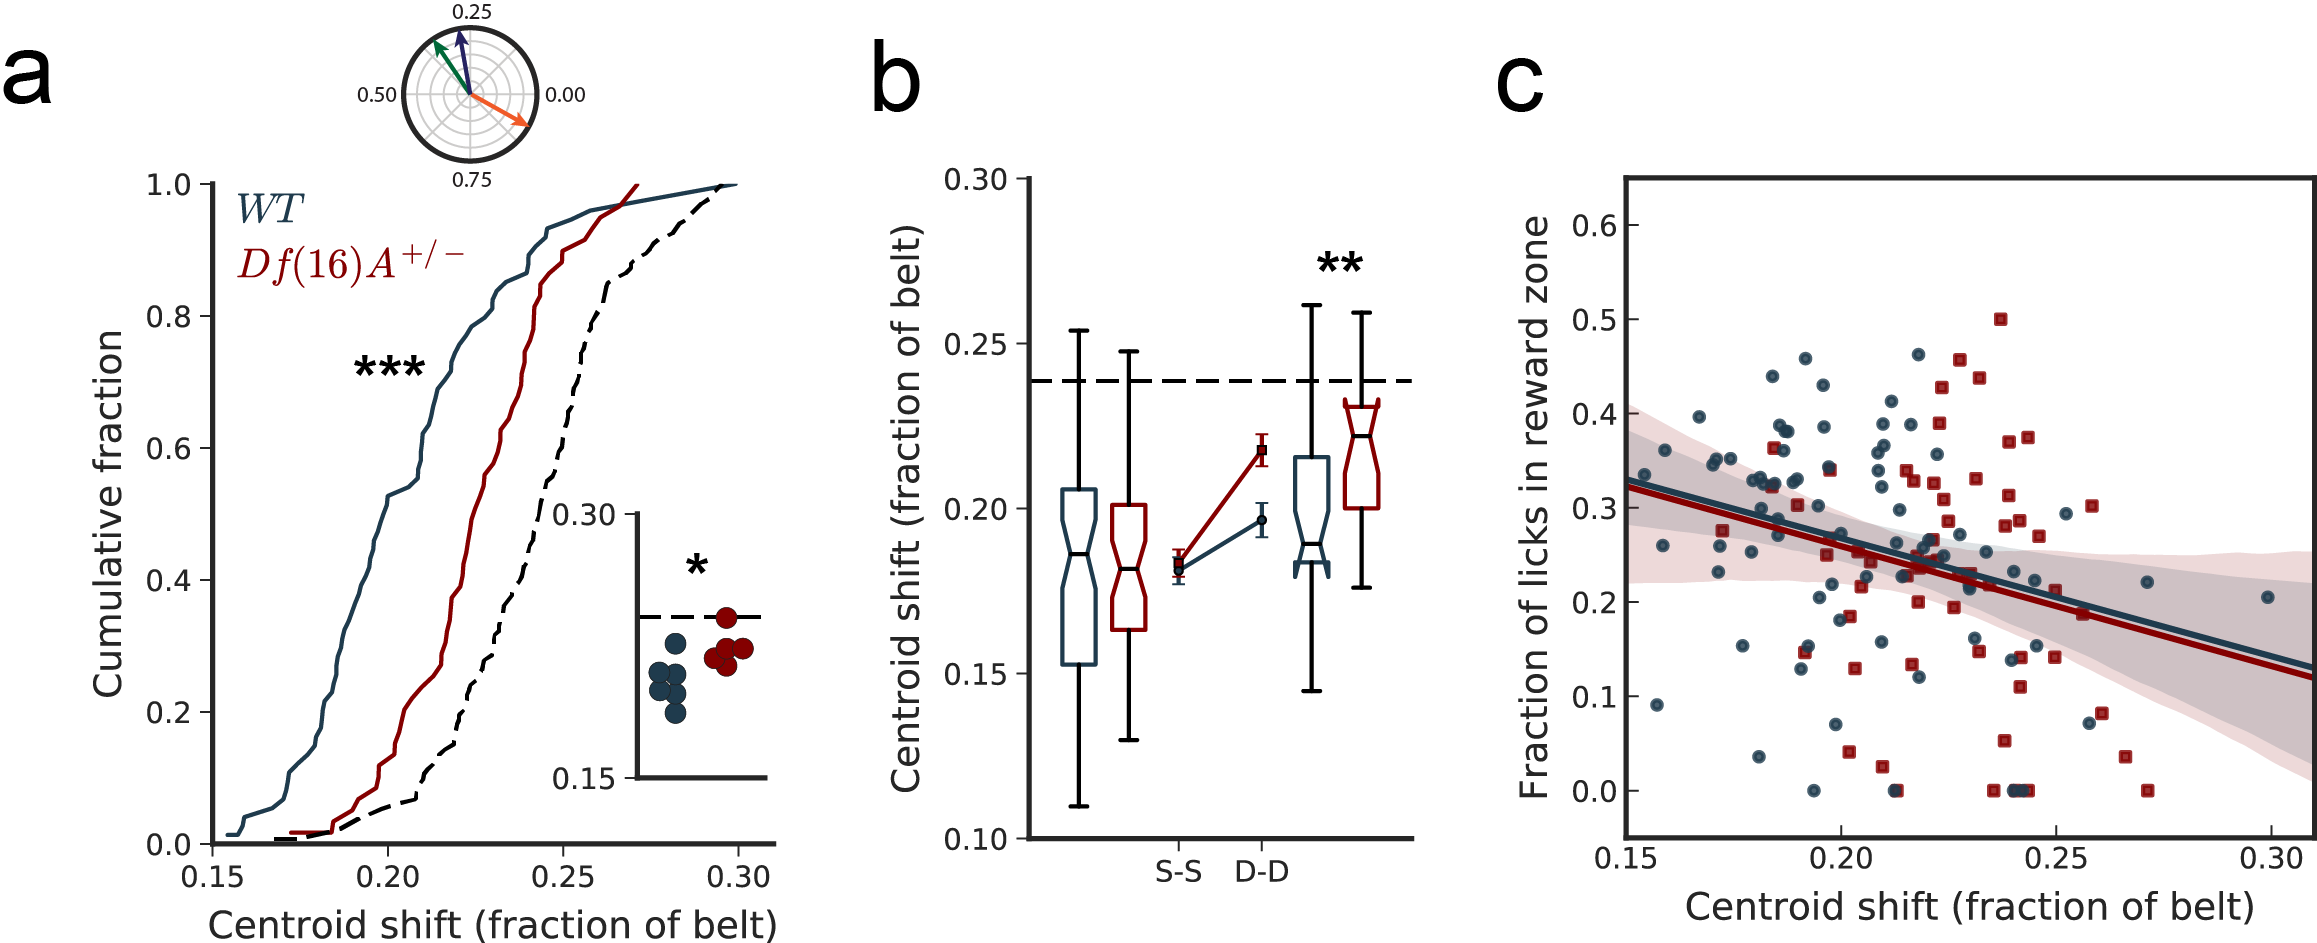
\includegraphics[width=0.8\textwidth]{df/Fig3_cent_shift}
	\caption[Comparison of centroid shift]{d. (top) Preferred spatial tuning is represented as a vector where the angle is the position on the treadmill of maximal activity. Across three sessions (green, blue, orange lines) spatial preference is generally stable (green to blue sessions), though salient events or changes to the environment can induce remapping (blue to orange session). The centroid shift is the angle between these vectors, represented as the fraction of the belt. (bottom) Distribution of mean centroid shift from day-to-day per session (dotted line is cell-identity shuffled distribution: WT: 0.204~$\pm$~0.003, n=74 sessions, \df/: 0.224~$\pm$~0.003, n=59 sessions, shuffle: 0.242~$\pm$~0.002, n=133; WT vs. shuffle: independent sample T-test, t=-9.42, p$<$0.0001; \df/ vs. shuffle: independent samples T-test, t=-4.25, p$<$0.0001; WT vs. \df/: independent samples T-test, t=-4.71, p$<$0.0001), and aggregated by mouse (inset, gray bar is cell-identity shuffle; independent samples T-test, t=2.58, p=0.0295).  e. Mean centroid shift from session-to-session (S-S) or day-to-day (D-D) for WT and \df/ mice (dotted line is mean centroid shift, two-way ANOVA for elapsed time and genotype; main effect of Genotype: F(1,152)=2.693, p=0.103; main effect of Time: F(1,152)=20.378, p$<$0.0001; Time $\times$ Genotype interaction: F(1,152)=3.340, p=0.0696; post-hoc analysis, WT vs. \df/, S-S: t=0.394, p=0.694; D-D: t=2.985, p=0.0047). f. Correlation of mean day-to-day stability with performance throughout the task. Solid line and shaded regions as in d (Pearson's correlation coefficient, WT: -0.306, p=0.008; \df/: -0.218, p=0.097; WT correlation vs. \df/ correlation, Fisher Z transformation of correlations, GLM model, Univariate Analysis of Variance: Genotype $\times$ Stability interaction: F(1,132)=0.268, p=0.605). *p$<$0.05, **p$<$0.01}
	\label{fig:df:cent_shift}
\end{figure}
\begin{figure}
	\centering
	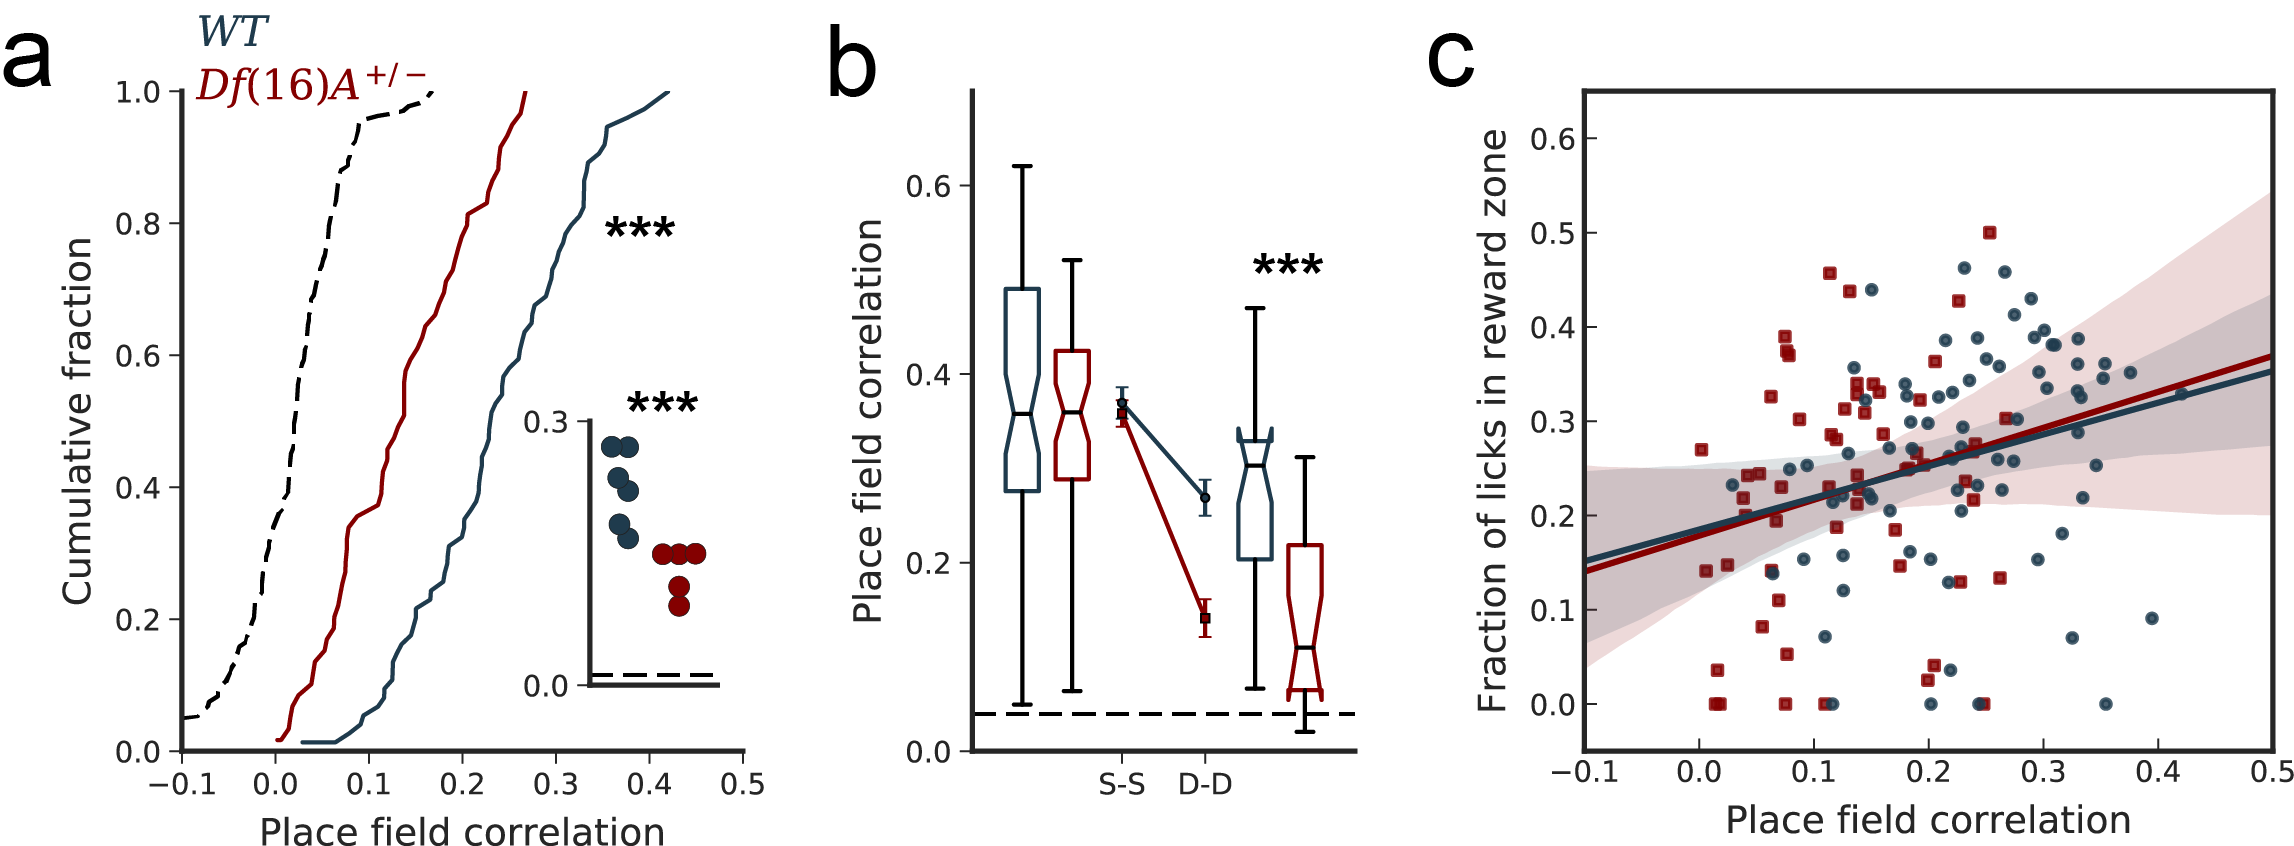
\includegraphics[width=0.8\textwidth]{df/FigS3_place_field_correlation}
	\caption[Comparison of place field correlation]{Place field correlation showed an overall similar effect as centroid shift (see \autoref{fig:df:cent_shift}). a. Compared to WT mice, \df/ mice show a significant overall decrease in place field correlation (WT: 0.232~$\pm$~0.010, n=74 sessions; \df/: 0.130~$\pm$~0.010, n=59 sessions; shuffle: 0.0238~$\pm$~0.005, n=133; WT vs. shuffle: Welch's T-test; t=18.87; p$<$0.0001; \df/ vs. shuffle: Welch's T-test, t=9.89, p$<$0.0001; WT vs. \df/, independent samples T-test, t=7.143, p$<$0.0001; inset aggregated by mouse: WT vs. \df/: independent samples T-test, t=2.584, p=0.0295). b. Place fields were more stable from session-to-session than day-to-day and the \df/ mice were less stable across elapsed time (two-way ANOVA for time elapsed and genotype, main effect of Genotype: F(1,152)=5.710, p=0.0181; main effect of Time: F(1,152)=55.329, p$<$0.0001; Time $\times$ Genotype interaction: F(1,152)=8.074, p=0.00511; S-S, WT vs. \df/f: t=0.507, p=0.613; D-D, WT vs. \df/: t=4.455; p$<$0.0001). c. Task performance correlates with the session-mean place field correlation for WT mice (Spearman's correlation coefficient=0.335, p=0.004) and trends similarly for \df/ mice (Pearson's correlation coefficient=0.224, p=0.088).}
	\label{fig:df:pf_corr}
\end{figure}

\subsection{Task performance correlates with spatial map stability}

Stability of place fields over time is thought to provide basis for spatial and episodic learning \citep{Kentros2004, Mankin2012, Thompson1990, Ziv2013}.
\todo[color=cyan]{These works could be cited and discussed in introductory chapter}
If so, we expect that the relative stability of these maps would reflect the ability of mice to perform in our GOL task. Indeed, on a per-session basis the overlap in the identity of place cells from day-to-day correlated with learning performance across all conditions of the GOL task for both groups (recurrence probability vs. fraction of licks in reward zone: Pearson's correlation coefficient, WT: 0.288, p=0.013; \df/: 0.416, p=0.001; \autoref{fig:df:recurrence}c), suggesting that this coding strategy is implemented by both WT and \df/ mice, though the overall decreased population stability in the \df/ mice contributes to the impaired task performance -- the \df/  mice are shifted lower on the recurrence-performance curve. In a similar manner to recurrence probability, place cell firing location stability also correlated with task performance for the WT mice and trended similarly in the \df/ mice (centroid shift vs. fraction of licks in reward zone: Pearson's correlation coefficient, WT: -0.306, p=0.008; \df/: -0.218, p=0.097; \autoref{fig:df:cent_shift}c; place field correlation; Spearman's correlation coefficient, WT: 0.335, p=0.004; Pearson's correlation coefficient, \df/: 0.224, p=0.088; \autoref{fig:df:pf_corr}c). In addition, as is suggested by the overall correlation of task performance with stability, the trajectory of these metrics by Condition mirrors the trajectory of the behavioral deficit in the task. Namely, just as we did not see a difference in behavior during Condition~I (\autoref{fig:df:trajectories}a, see \autoref{fig:df:task_performance}), stability is also similar between WT and \df/  mice during Condition~I, but while the WT place cell population continues to stabilize in Condition~II and III, the \df/ population stability drops off as the task demands change (\autoref{fig:df:trajectories}b: two-way ANOVA, main effect of Genotype, p=0.048; Genotype $\times$ Condition interaction, p=0.083; post-hoc analysis comparing genotype, Condition~I and II, n.s., Condition~III, p=0.016). Thus, the learning strategy employed by both genotypes does involve the formation and maintenance of stable hippocampal spatial maps, but the stability of these maps is impaired in \df/ mice -- particularly from day-to-day and when the task demands change -- as reflected in their decreased performance on the GOL task.

\begin{figure}
	\centering
	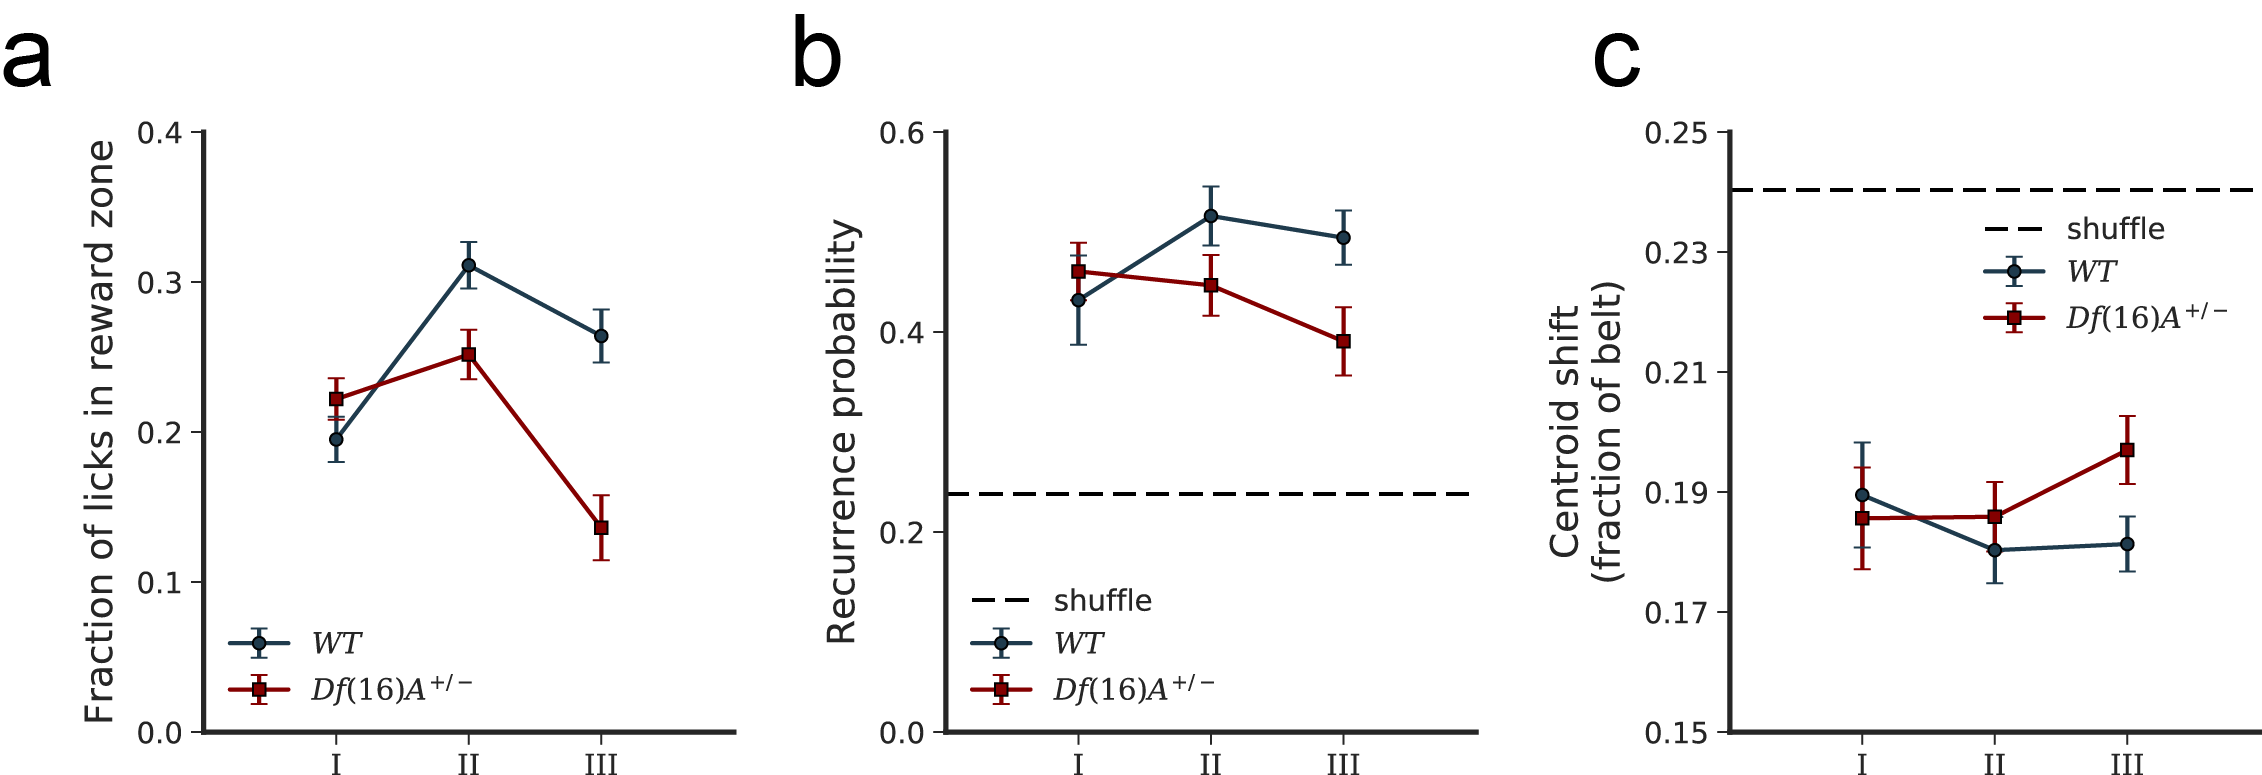
\includegraphics[width=0.8\textwidth]{df/Fig3_trajectories}
	\caption[Task performance and population stability follow similar trajectories across Conditions]{Task performance and population stability by genotype follows similar trajectories across Conditions; that is to say, performance and stability are similar in Condition~I, slightly impaired in the \df/ mice during Condition~II and most different during Condition~III (three-way ANOVA, Genotype $\times$ Metric $\times$ Condition interaction: F(4,549)=0.484, p=0.747; Condition $\times$ Genotype interaction: F(2,549)=11.982, p=$<$0.0001; Metric $times$ Genotype interaction: F(2,549)=0.771, p=0.463; Metric $\times$ Condition interaction: F(4,549)=1.503, p=0.200; Condition~I, all metrics, WT vs. \df/: independent samples T-test: t=-1.194, p=0.234; Condition~II, all metrics, WT vs. \df/: independent samples T-test: t=2.67, p=0.0081; Condition~III, all metrics, WT vs. \df/: Welch's T-test: t=5.586, p$<$0.0001). a. Fraction of licks in the reward zone by condition (two-way ANOVA, main effect of Genotype p$<$0.0001, main effect of Condition p$<$0.0001, Genotype $\times$ Condition interaction p$<$0.0001). b. Recurrence probability by condition (two-way ANOVA, main effect of Genotype p=0.048, main effect of Condition p=0.505, Genotype $\times$ Condition interaction p=0.083). c. Mean centroid shift by condition (two-way ANOVA, main effect of Genotype p=0.284, main effect of Condition p=0.620, Genotype $\times$ Condition interaction p=0.347).}
	\label{fig:df:trajectories}
\end{figure}

\subsection{Goal-oriented learning requires dorsal hippocampal area CA1 and relies on allocentric navigational strategies}

To confirm the necessity of the hippocampus to our GOL task, we pharmacologically silenced bilateral dorsal hippocampus area CA1 using the GABAA-receptor agonist muscimol during initial learning of a fixed reward location. Mice ran in a single Condition (same reward location, belt, local cues, and non-spatial cues, identical to the initial learning conditions of Condition~I) for 4 days (3 sessions per day) with the first group of mice receiving a bilateral local infusion of muscimol to dorsal hippocampus 30 minutes before the start of the first trial for the first 3 days and then saline on the fourth day. The second group of mice was infused with saline for the first 3 days and then muscimol on the fourth day. Mice in which their dorsal hippocampus was silenced during initial learning of the reward location performed significantly worse than mice with an active hippocampus (Days 1-3, muscimol to saline vs. saline to muscimol: p$<$0.0001; \autoref{fig:df:muscimol}), indicating that silencing dorsal hippocampus activity results in decreased ability to learn a hidden reward zone. On the fourth day, the mice that had received muscimol infusions now received saline infusions and these mice still perform poorly on the task, showing that the silencing of the hippocampus was not merely suppressing the expression of goal oriented learning, but that instead they are just beginning to learn the reward location. In further support of the hippocampal-dependence of this task, mice that successfully learned the task with an active hippocampus over the first three days had their dorsal hippocampus silenced during the fourth day and showed a significant decrease in goal oriented behavior (saline to muscimol, Days 1-3 vs. Day 4: p=0.0235), and now performed similar to the initially silenced training group (Day 4, saline to muscimol vs. muscimol to saline: p=0.535).

\begin{figure}
	\centering
	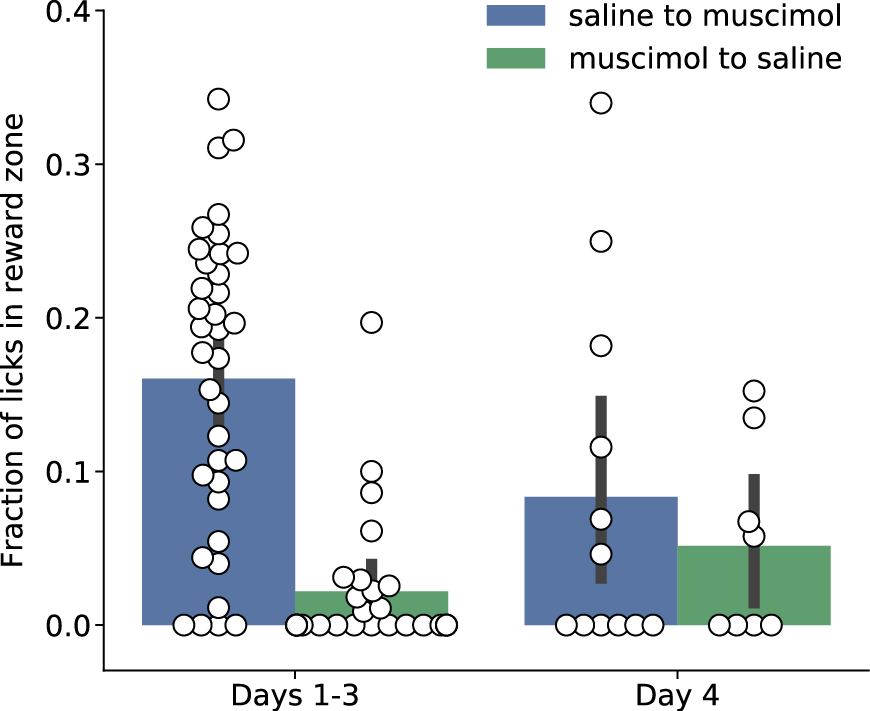
\includegraphics[width=0.5\textwidth]{df/FigS5_muscimol_inactivation}
	\caption[Impaired task performance during CA1 inactivation]{During initial learning of a reward location, local inactivation of CA1 lead to significantly reduced task performance (Days 1-3, muscimol to saline vs. saline to muscimol: Mann-Whitney U, U=126.5, p$<$0.0001). In addition, mice which received saline infusion during the first three initial learning days performed significantly worse on the fourth day when they were infused with muscimol (saline to muscimol, Days 1-3: 0.221~$\pm$~0.053, n=36 sessions; Day 4: 0.084~$\pm$~0.034, n=12 sessions; Mann-Whitney U, U=111, p=0.0235) and now performed at a similar level to mice which were initially infused with muscimol (Day 4, saline to muscimol vs. muscimol to saline: independent samples T-test, t=0.633, p=0.535).}
	\label{fig:df:muscimol}
\end{figure}

Allocentric and path integration navigational strategies are thought to be two complementary attributes of the hippocampal-entorhinal navigational-memory circuitry \citep{Buzsaki2013, Etienne2004, Gothard1996, Moser2015}. While in our head-fixed GOL task, local cues and fabric segments of the treadmill belt are aimed to primarily provide an allocentric reference frame for spatial map during learning, mice can in principle also use egocentric, path integration strategies to find the reward location. In order to elucidate the relative contribution of allocentric navigation and path integration in the learning task, we carried out experiments in which we imaged WT mice in the absence of local cues on the treadmill belt, where we find that place cells were practically absent (place cell fraction, cue-rich vs. cue-free: p=0.004; \autoref{fig:df:not_path}a,b) and the tuning of all cells was significantly more diffuse (circular variance, cue-rich vs. cue-free: p$<$0.0001; \autoref{fig:df:not_path}c). Furthermore, in the case of path integration, we would expect that during transition between Condition~I and II, when fabric transitions are the only features remaining constant, place cells near the fabric transitions would be more stable than place cells farther from the fabric transitions, as errors in path integration would accumulate with distance \citep{Etienne2004, Gothard1996}. We carried out analyses in which we compared the stability of spatial tuning from the last day of Condition~I to the first session of Condition~II by dividing cells into three groups based on which third of the treadmill belt they were active in at the end of Condition~I -- before the fabric transitions, after the fabric transitions, and in the middle of the fabric segments. We found no difference in stability contributable to the distance of the initial preferred tuning to the nearest fabric transition (two-way ANOVA, main effect of Binned Distance: p=0.977; \autoref{fig:df:not_path}d). These results together suggest that egocentric navigational strategies would be insufficient to maintain place cell firing, and thus mice indeed primarily employ allocentric navigational strategies for learning in the head-fixed GOL task.

\begin{figure}
	\centering
	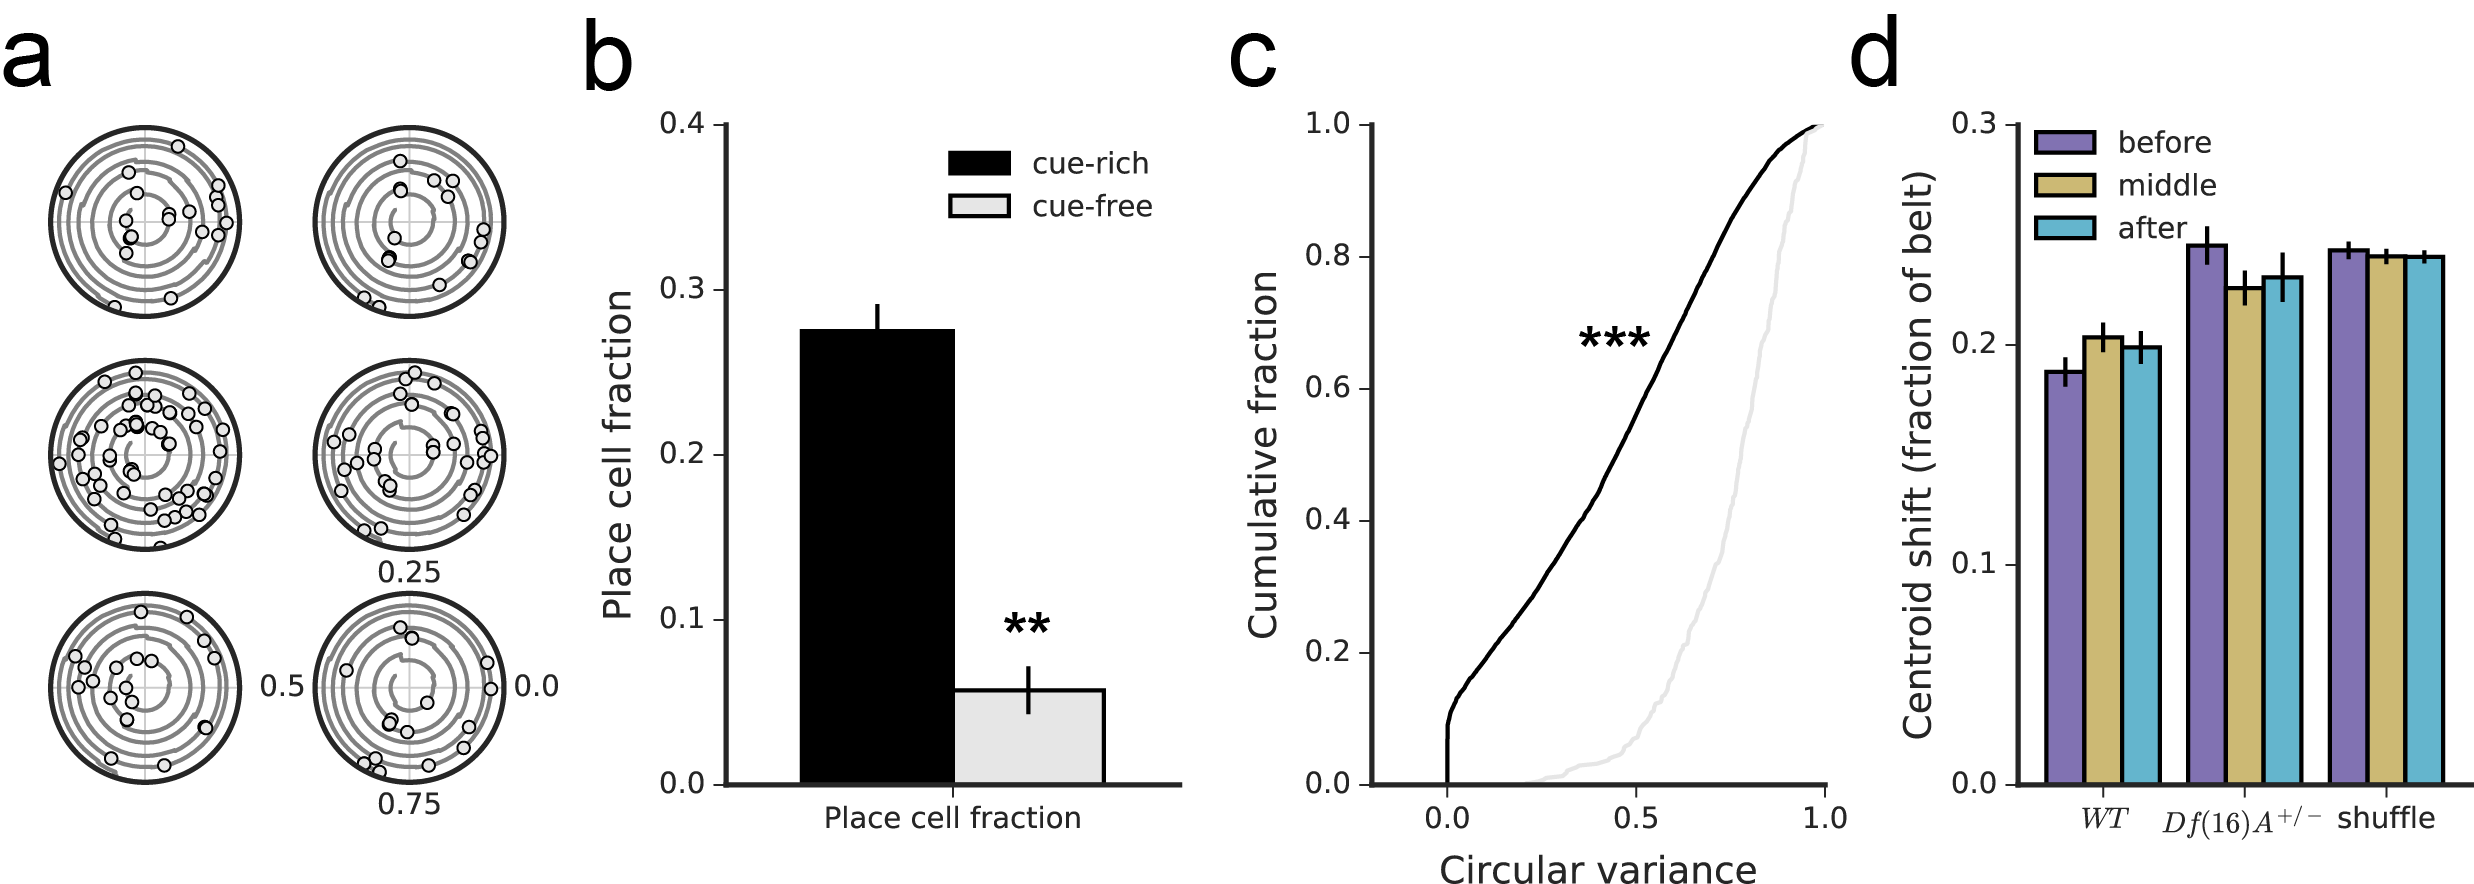
\includegraphics[width=0.9\textwidth]{df/FigS6_not_path_integration}
	\caption[No place cells on a cue-free belt and spatial tuning near the fabric-transition is not more stable]{a. The 6 most spatially tuned cells (lowest circular variance) on a burlap belt, plotted as in \autoref{fig:df:place_cells}.
	b. Place cell fraction on a `cue-rich' and `cue-free' belt during RF (cue-rich: 0.275~$\pm$~0.017, n=56 sessions; cue-free: 0.057~$\pm$~0.018, n=3 sessions; independent samples T-test, t=3.006, p=0.004).
	c. Transient circular variance on a `cue-rich' and `cue-free' belt during RF (cue-rich: 0.427~$\pm$~0.003, n=7828 cell*sessions; cue-free: 0.746~$\pm$~0.008, n=375 cell*sessions; Mann-Whitney U, U=$4.99\times10^5$, p$<$0.0001). d. Centroid shift of cells from the last day of Condition~I to the first session of Condition~II separated by tuning preference relative to fabric transitions -- the only features that remain constant between the two contexts. WT tuning is generally more stable (WT vs. \df/, independent samples T-test: t=-4.96, p$<$0.0001; see \autoref{fig:df:context_stability}), but neither genotype shows increased stability near the fabric transitions (two-way ANOVA, main effect of binned Distance: F(2,24)=0.024, p=0.977). *p$<$0.05, ***p$<$0.001}
	\label{fig:df:not_path}
\end{figure}

\subsection{Disrupted sharp wave-ripple activity in \df/ mice}
\label{sec:df:results:SWR}
Decreased task performance following long-delays (overnight period) coupled with the decreased recurrence and similarity of neuronal ensemble activity from day-to-day suggests a consolidation deficit in the \df/ mice. Reactivation and consolidation of memories of previous experiences are thought to occur during sharp wave-ripples (SWRs) -- large-amplitude, short-duration, high-frequency events detected in the local field potential \citep{Buzsaki2015, Diba2007, Dupret2010a, Foster2006, Jadhav2012, Kudrimoti1999, Wilson1994} during quiet wakefulness and sleep. To assess SWR activity in WT and \df/ mice, in a separate cohort of mice we implanted electrodes in hippocampal area CA1 to record the local field potential and detect SWRs (\autoref{fig:df:spectograms}a,b, see \autoref{sec:df:methods:SWR}) during a head-fixed random foraging task on a featureless burlap belt. During periods of immobility, we found that \df/ mice had significantly more SWRs (p$<$0.001; \autoref{fig:df:SWR_metrics}a), though the SWRs were irregular, as reflected by a higher mean ripple band-power (p$<$0.001; \autoref{fig:df:SWR_metrics}b) and a higher peak frequency in the ripple-band (p$<$0.001; \autoref{fig:df:SWR_metrics}c). To ensure the robustness of the result, we varied the SWR detection threshold and found that these effects held across SWR event detection thresholds (significance as noted in figure; \autoref{fig:df:SWR_thresholds}). Dysregulation of hippocampal excitability during periods of rest in \df/ mice, as manifest by increased SWR frequency and power, provides a possible mechanism behind the failure to efficiently retain a memory of the reward location by the \df/ mice.

\begin{figure}
	\centering
	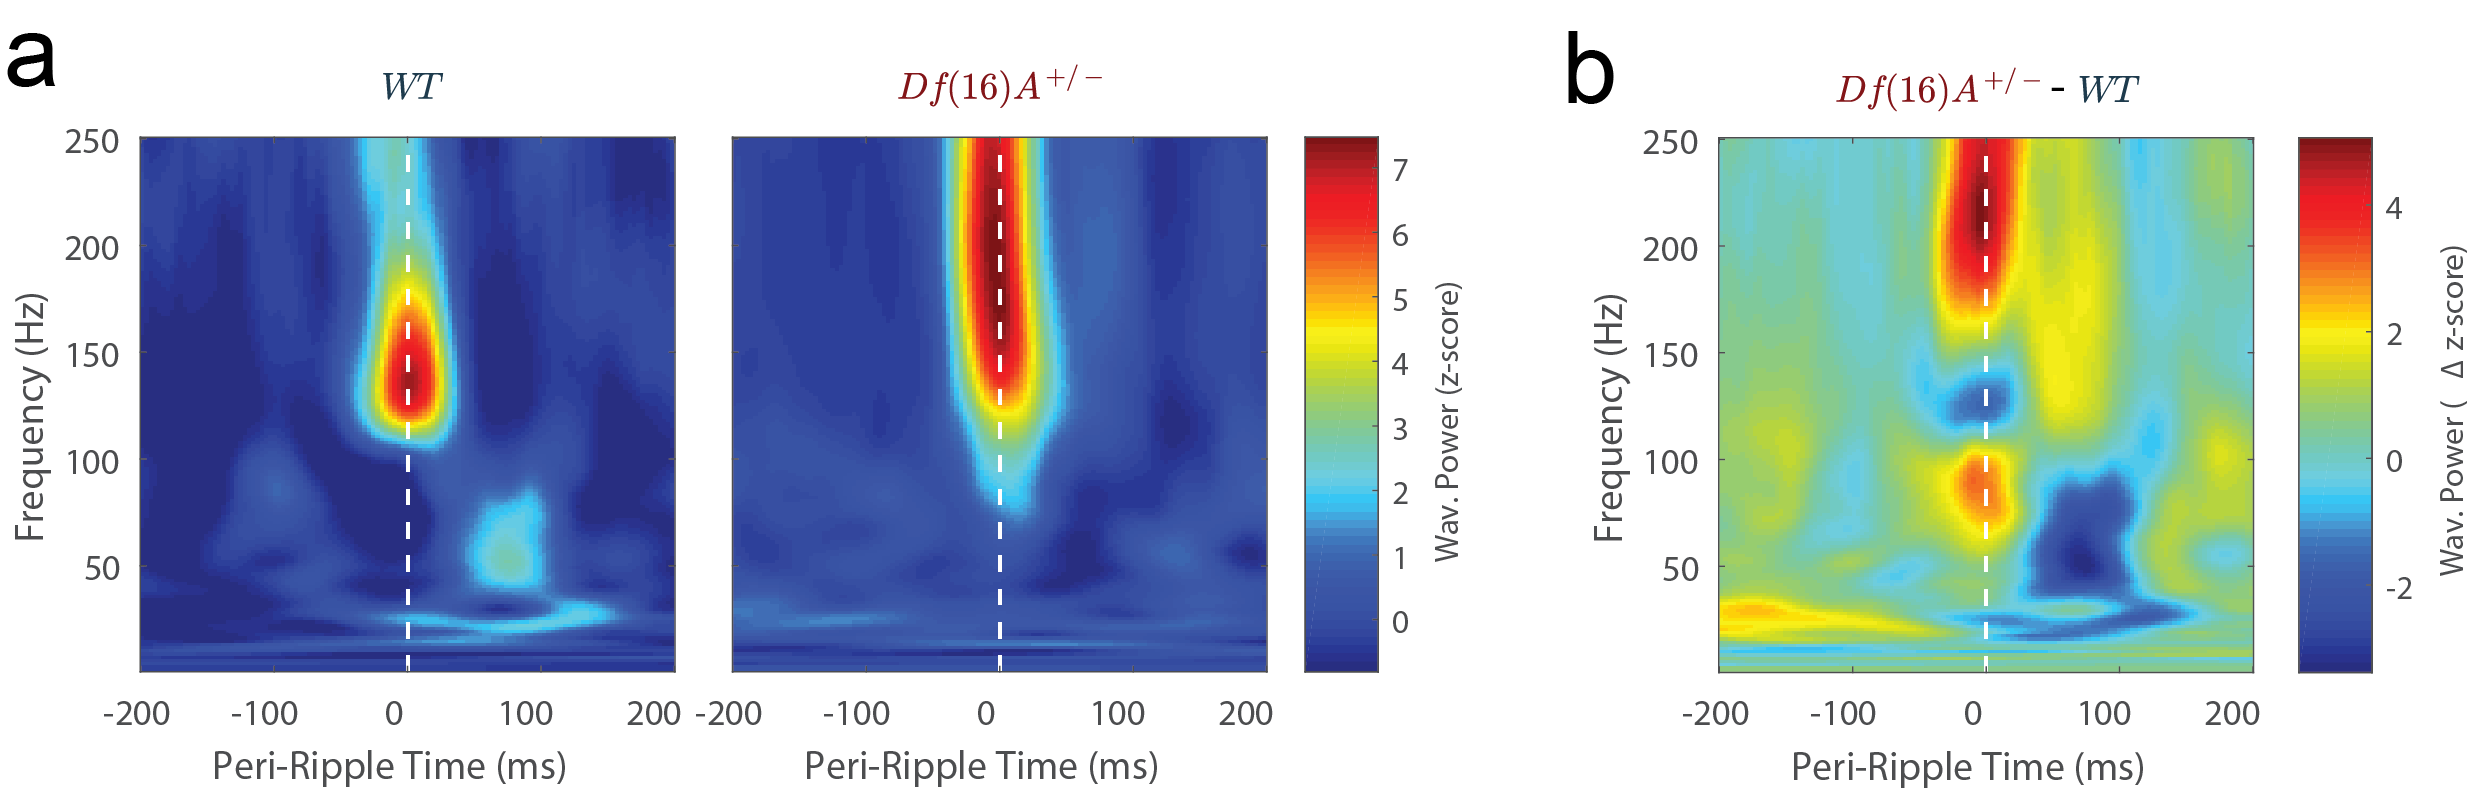
\includegraphics[width=0.9\textwidth]{df/FigS7_spectograms}
	\caption[Sharp wave-ripple spectrograms in WT and \df/ mice]{a. Mean SWR wavelet power for WT (left) and \df/ (right) mice.
	b. Difference (\df/ - WT) of mean SWR wavelet power in \emph{a}.}
	\label{fig:df:spectograms}
\end{figure}

\begin{figure}
	\centering
	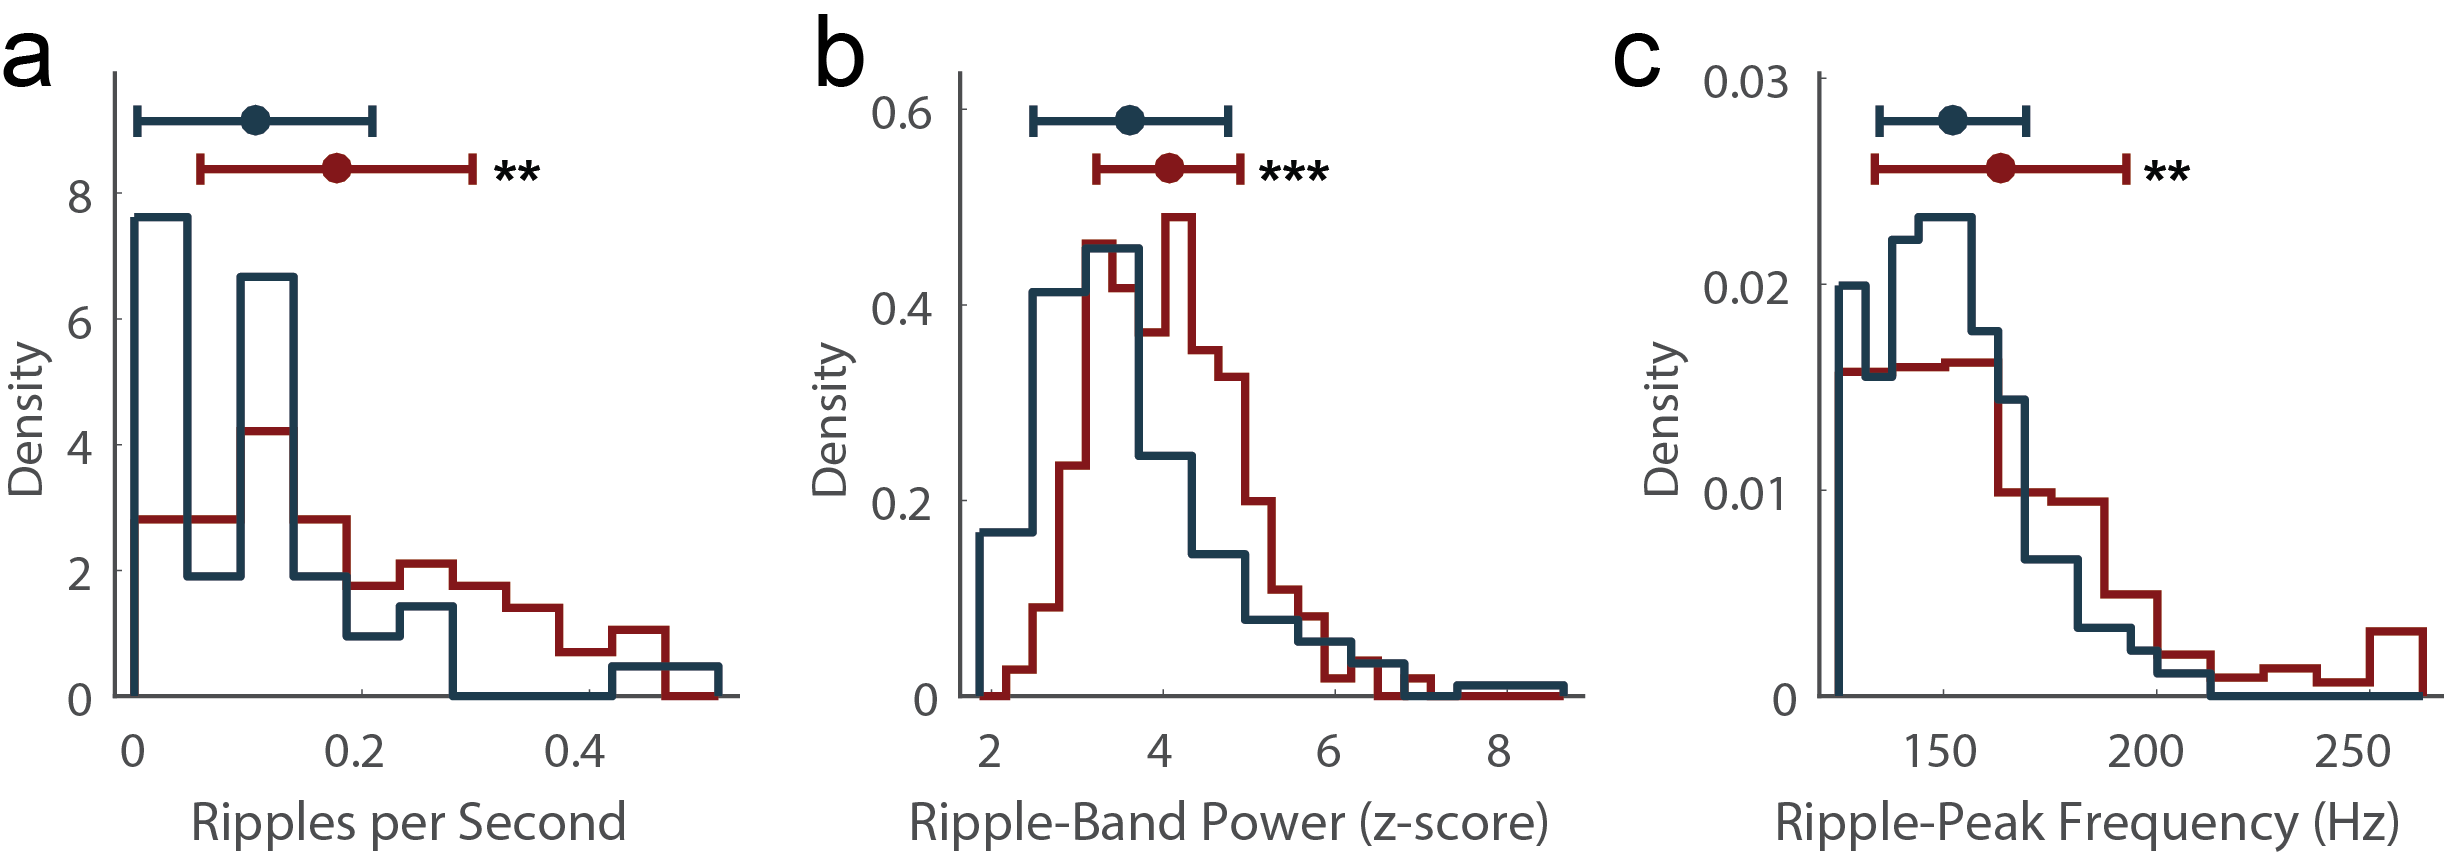
\includegraphics[width=0.9\textwidth]{df/FigS7_SWR_metrics}
	\caption[Rate and power of SWRs in WT and \df/ mice]{a. Rate of SWRs during stationary bouts (mean~$\pm$~SD; WT: 0.106~$\pm$~0.103, n=45 stationary intervals; \df/: 0.178~$\pm$~0.120, n=61 stationary intervals; Wilcoxon rank-sum test, h=3777.5, p=0.00096).
	b. Mean wavelet power (mean~$\pm$~SD; WT: 3.622~$\pm$~1.133, n=145 sharp-wave ripples; \df/: 4.060~$\pm$~0.838, n=357 sharp wave-ripples; Wilcoxon rank-sum test, h=98423, p$<$0.0001).
	c. Frequency with maximum power (mean~$\pm$~SD; WT: 152.190~$\pm$~17.174, n=145 sharp wave-ripples; \df/: 163.391~$\pm$~29.485, n=357 sharp wave-ripples; Wilcoxon rank-sum test, h=94798, p=0.00066).}
	\label{fig:df:SWR_metrics}
\end{figure}

\begin{figure}
	\centering
	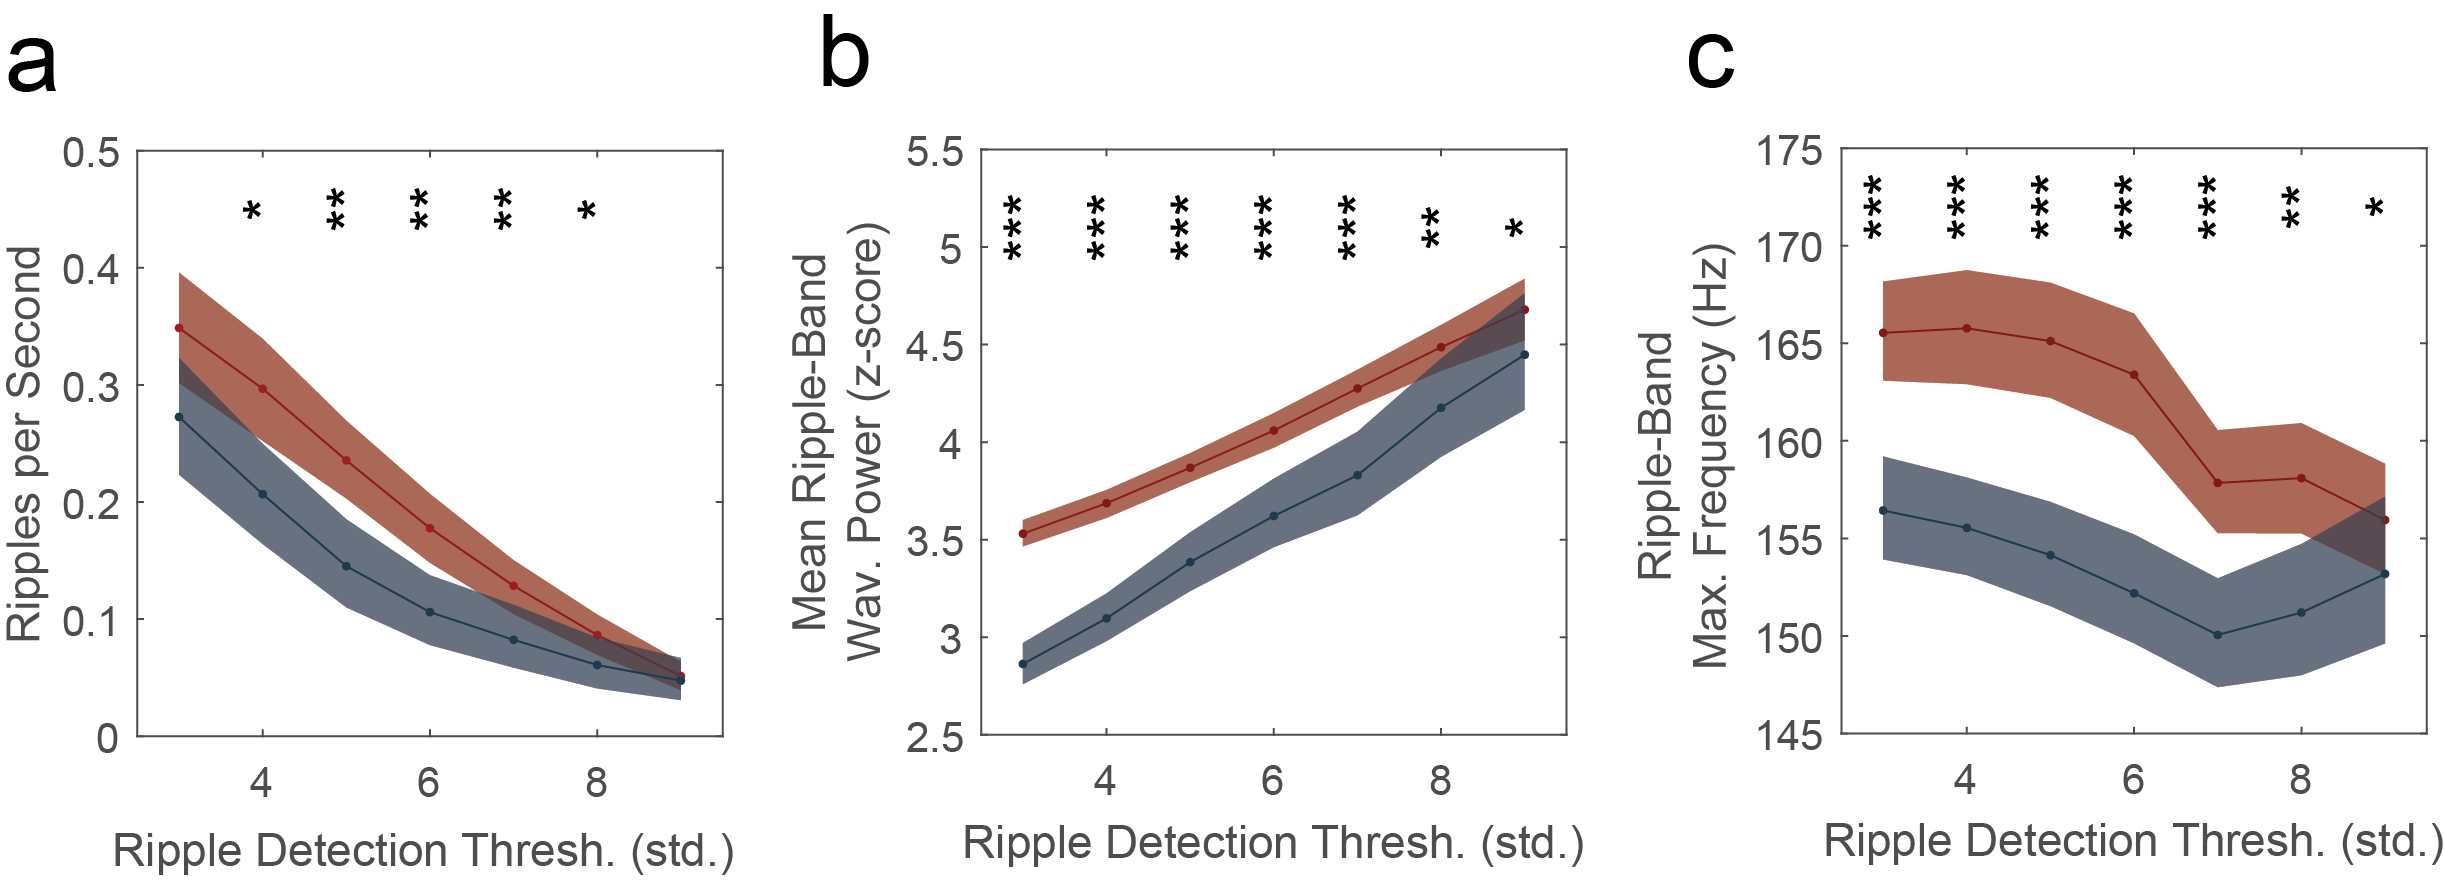
\includegraphics[width=0.9\textwidth]{df/FigS7_SWR_thresholds}
	\caption[SWR properties at multiple thresholds]{Same as \autoref{fig:df:SWR_metrics} for several SWR detection thresholds (significance by Wilcoxon rank-sum test as marked). *p$<$0.05, **p$<$0.001, ***p$<$0.0001}
	\label{fig:df:SWR_thresholds}
\end{figure}

\subsection{Change in context induces disrupted place cell stability in \df/ mice}
\label{sec:df:results:context}
In addition to deficits following the overnight period, \df/ mice showed significantly impaired performance after a change in context during Condition~II in the GOL task (Condition~II, Day~1; see Figures \ref{fig:df:licktograms} \& \ref{fig:df:task_performance}) -- a change in both the non-spatial (tone, light, and odor) and proximal spatial cues (shuffled local cues on belt, constant fabric sequence). When we compared the day-to-day stability of place fields in WT and \df/ mice across this transition (Condition~I-Day~3 to Condition~II-Day~1) we found that place fields in WT mice were significantly more stable than in \df/ mice (p=0.0055; \autoref{fig:df:context_stability}a). Since this change of local cues from Condition~I to Condition~II dissociates `position' relative to the sequence of fabrics and `position' relative to the cues, we looked at coding of space relative to these two distinct reference frames in the WT and \df/ mice. First, we looked at all the place cells that were active near a cue on the last day of Condition~I and asked if on the first day in Condition~II it fired closer to that same cue (`cue-preferring') or the position relative to the fabric sequence where the cue was previously (`position-preferring', see Methods). We found a significantly different distribution of cue-preferring and position-referring cells between WT and \df/ mice (p$<$0.0001; \autoref{fig:df:context_stability}b), with notably fewer position-preferring cells in the \df/ mice and a significantly lower ratio of cue- to position-preferring cells (p=0.0131; \autoref{fig:df:context_stability}c). Again, importantly, in Condition~II the location of the hidden reward does not change relative to the fabric sequence, so the lack of cells that track `position' in the \df/ mice is consistent with the increased disruption in task performance and the decreased stability of the population relative to the fabric sequence in the \df/ mice. Thus, we see that changes to the non-spatial context and the shuffling of local cues induced remapping and disrupted the stability of spatial maps in \df/ mice significantly more than in WT mice, and in particular, fewer cells remained anchored to the belt reference space.

\begin{figure}
	\centering
	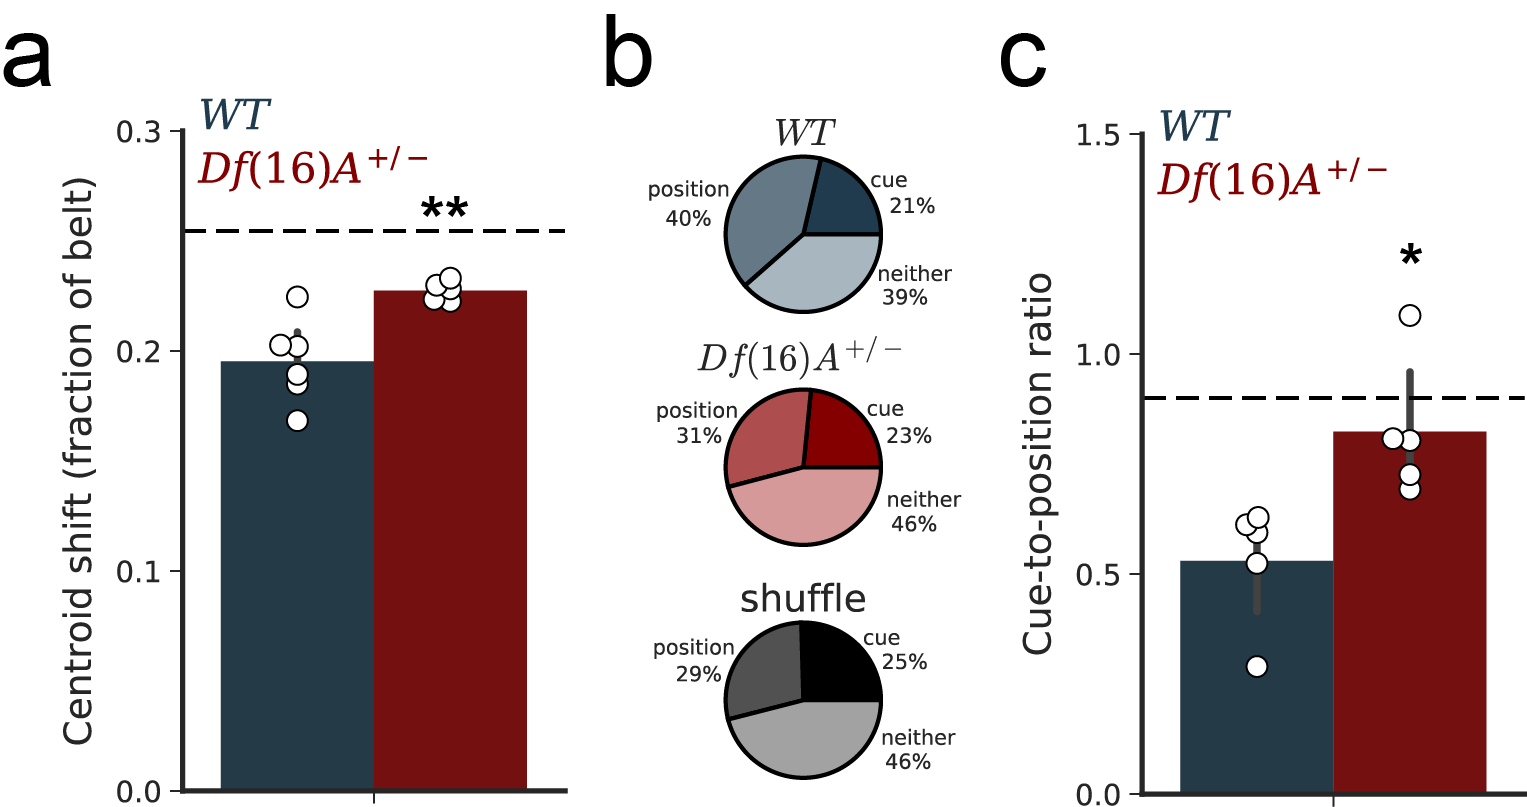
\includegraphics[width=0.7\textwidth]{df/Fig4_context_stability}
	\caption[Subtle contextual change induces remapping in \df/ mice]{a. Mean centroid shift from the last day of Condition~I to the first day of Condition~II (WT: 0.195~$\pm$~0.008, n=6; \df/: 0.227~$\pm$~0.002, n=5; independent samples T-test: t=-3.626, p=0.0055).
	b. Fraction of all cells classified as place-preferring, cue-preferring, or neither (pooled across mice) for WT, \df/ and shuffled data (Pearson chi-square test: $\chi^2$=85.7776, p$<$0.0001).
	c. Ratio of the number of cue-preferring to place-preferring cells per mouse for WT and \df/ mice (independent samples T-test: t=-3.172, p=0.0131). *p$<$0.05, **p$<$0.01}
	\label{fig:df:context_stability}
\end{figure}

\subsection{Task-dependent stabilization of place cell populations is impaired in \df/ mice}
\label{sec:df:results:rf}
To better understand the conditions in which place cell stability is affected in the \df/ mice, we next aimed to separate baseline place cell stability from the demands of a spatial learning task.  In a separate random foraging (RF) paradigm, where there is no learning of a particular reward position involved, we trained water-deprived mice to run head-fixed on a similar cue-rich belt. In this task the reward schedule was changed such that water was presented to the mice probabilistically as they ran, independent of both position on the belt and whether or not they lick (\autoref{fig:df:RF}a). From day-to-day, preferred firing locations were more stable than expected by chance in both WT and \df/ mice (WT: 0.222~$\pm$~0.004, n=30 session pairs; \df/: 0.220~$\pm$~0.004, n=42 session pairs; shuffle: 0.244~$\pm$~0.002, n=72; WT vs. shuffle: p$<$0.0001; \df/ vs. shuffle: p$<$0.0001), but in contrast to during the GOL task, they were not significantly different from each other (WT vs \df/: p=0.653; \autoref{fig:df:RF}b). More specifically, the WT spatial tuning is significantly stabilized in the GOL task while the \df/ spatial tuning is not (two-way ANOVA, Genotype $\times$ Task interaction, p=0.0322, main effects, n.s.; WT, GOL vs. RF: p=0.022; \df/, GOL vs. RF: p=0.579; \autoref{fig:df:RF}c). This suggests that the presence of a spatially-salient reward location selectively stabilizes hippocampal spatial masks in WT mice, a phenomenon absent from \df/ mice.

\begin{figure}
	\centering
	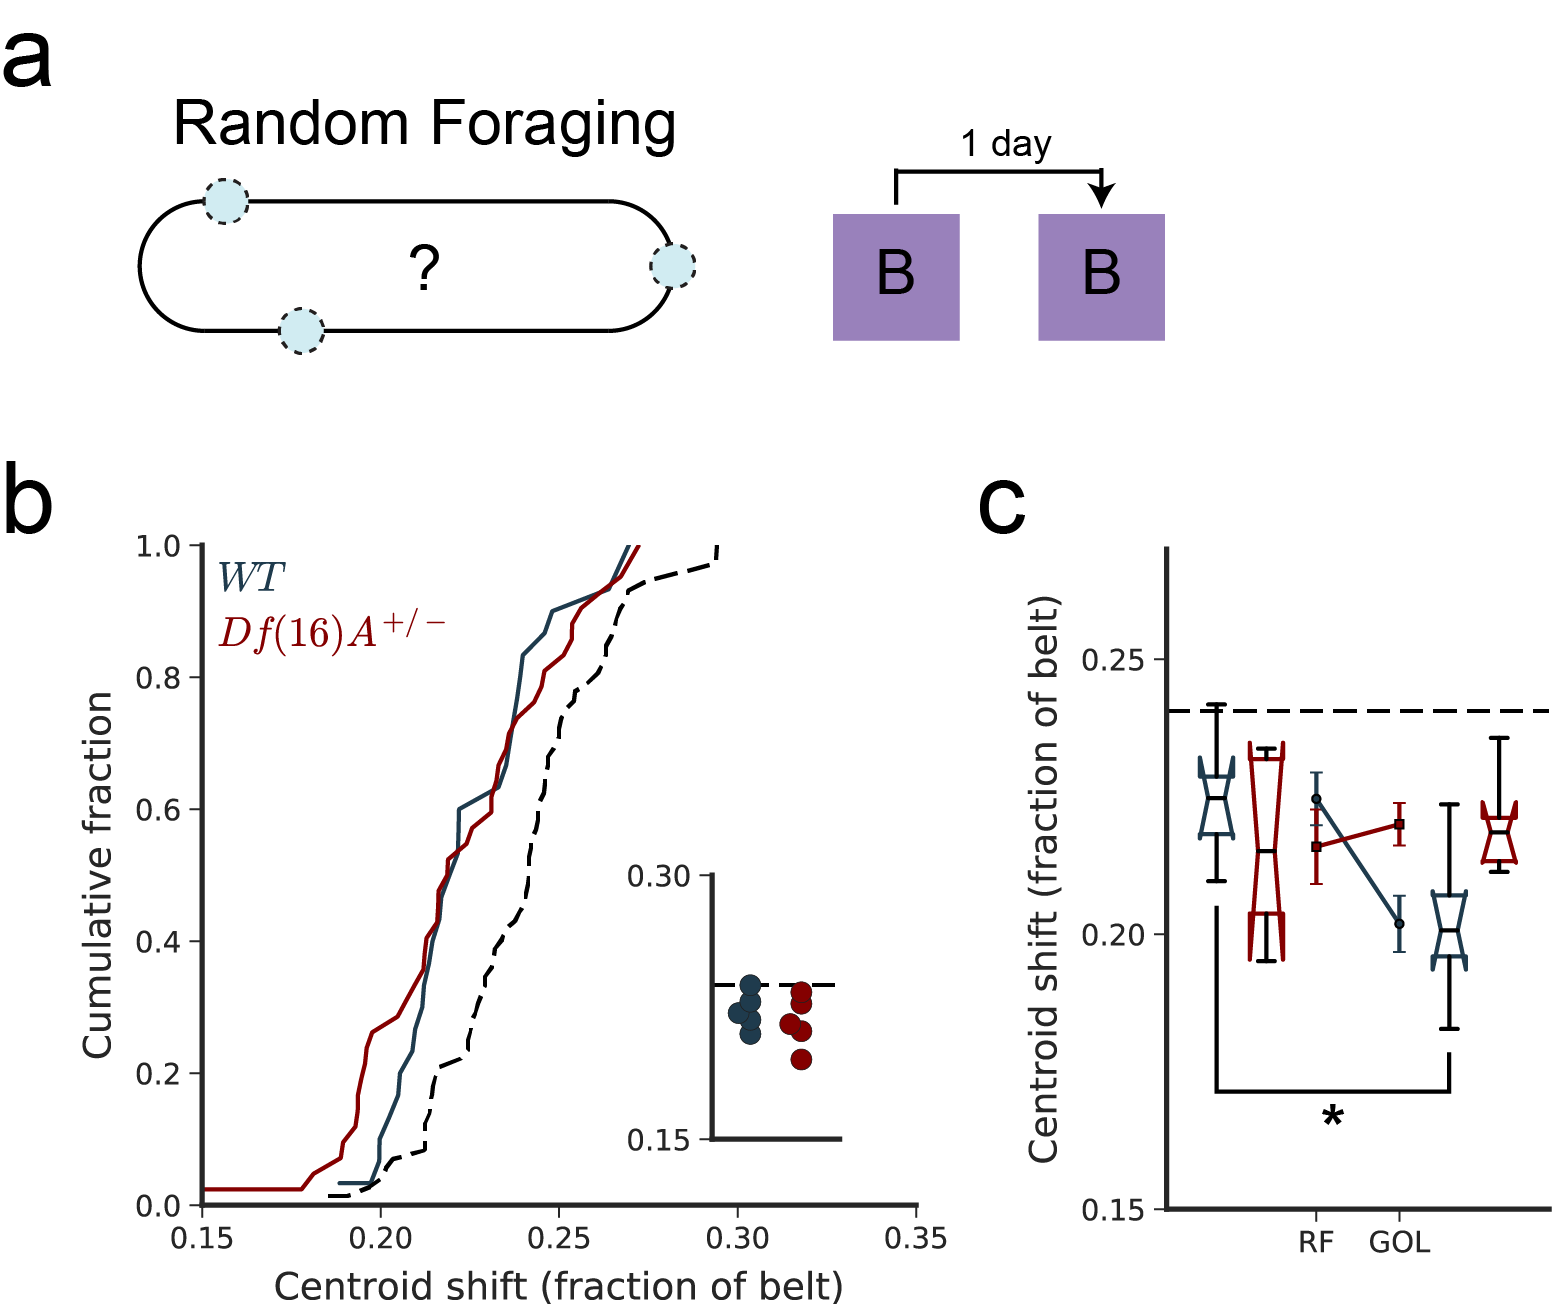
\includegraphics[width=0.7\textwidth]{df/Fig4_rf}
	\caption[Lack of task-dependent stability of spatial maps in \df/ mice]{a. Schematic of Random Foraging (RF) task. Rewards are presented randomly throughout the belt in the same context: same belt fabric sequence, different auditory, visual, olfactory, and tactile cues.
	b. Distribution of mean centroid shift per session from day-to-day during Random Foraging task (dotted line is cell-identity shuffled distribution; WT: 0.222~$\pm$~0.004, n=30 session pairs; \df/: 0.220~$\pm$~0.004, n=42 session pairs; shuffle: 0.244~$\pm$~0.002, n=72; WT vs. shuffle: independent sample T-test: t=-5.05, p$<$0.0001; \df/ vs. shuffle: Welch's T-test, t=-5.12, p$<$0.0001; WT vs \df/: independent samples T-test: t=0.451, p=0.653) and aggregated by mouse (inset, gray bar is cell-identity shuffle; WT vs. \df/: independent samples T-test: t=0.799, p=0.448).
	c. Comparison of mean centroid shift per mouse in the RF and GOL tasks (GOL data replotted from \autoref{fig:df:cent_shift}b; two-way ANOVA, Genotype $\times$ Task interaction, p=0.0322, main effects, n.s.; WT, GOL vs. RF: p=0.022; \df/, GOL vs. RF: p=0.579). *p$<$0.05}
	\label{fig:df:RF}
\end{figure}

\subsection{Enrichment of goal location by place cells in WT, but not \df/ mice}
\label{sec:df:results:enrichment}
Place maps incorporate goal-related information during learning \citep{Breese1989, Dupret2010b, Fyhn2002, Gothard1996, Hok2007, Hollup2001b, Kobayashi1997}, and over-representation of goal locations by place cells has been shown to correlate with learning performance during goal-directed spatial learning tasks \citep{Dupret2010a, Hollup2001b}.  While we did not observe place cell enrichment during initial goal learning in a novel context (Condition~I) or the subsequent change of context (Condition~II), upon learning of the new reward location in an already familiar context (Condition~III), we found robust organized remapping of place cells towards the new reward location in WT mice, though this goal-directed reorganization was strikingly absent in \df/ mice (two-way RM ANOVA: Genotype $\times$ Condition $\times$ Day interaction: p$<$0.0001; Conditions~I \& II: no significant effect of Genotype:  p=0.749 and p=0.065, respectively; Condition~III, Genotype $\times$ Day interaction: p$<$0.0001; main effect of Genotype: p=0.002; post-hoc analysis with Bonferroni correction for multiple comparisons, Day 3: p$<$0.0001; Figures \ref{fig:df:enrich_heatmaps} \& \ref{fig:df:enrichment}).  Additionally, we found that the magnitude of place cell enrichment at the goal location correlated with learning performance in WT mice (Pearson Correlation, Z=0.362, p=0.023; \autoref{fig:df:enrich_corr}) but not in \df/ mice (Pearson Correlation, Z=-0.068, p=0.791; \autoref{fig:df:enrich_corr}). The lack of enrichment during certain phases of our GOL task -- Conditions~I and II for WT mice and all Conditions for \df/ mice -- suggests that the learning performance is primarily determined by the initial formation and maintenance of stable spatial maps during these Conditions (see Figures \ref{fig:df:recurrence}, \ref{fig:df:cent_shift}, \& \ref{fig:df:pf_corr}), though an alternative, improved, goal-enrichment strategy is available to WT mice. Thus, place cell enrichment supports learning of new reward locations in a familiar context in WT animals, while in \df/ mice enrichment does not influence task performance, which may account for their significantly worse performance during this phase of the GOL task.

\begin{figure}
	\centering
	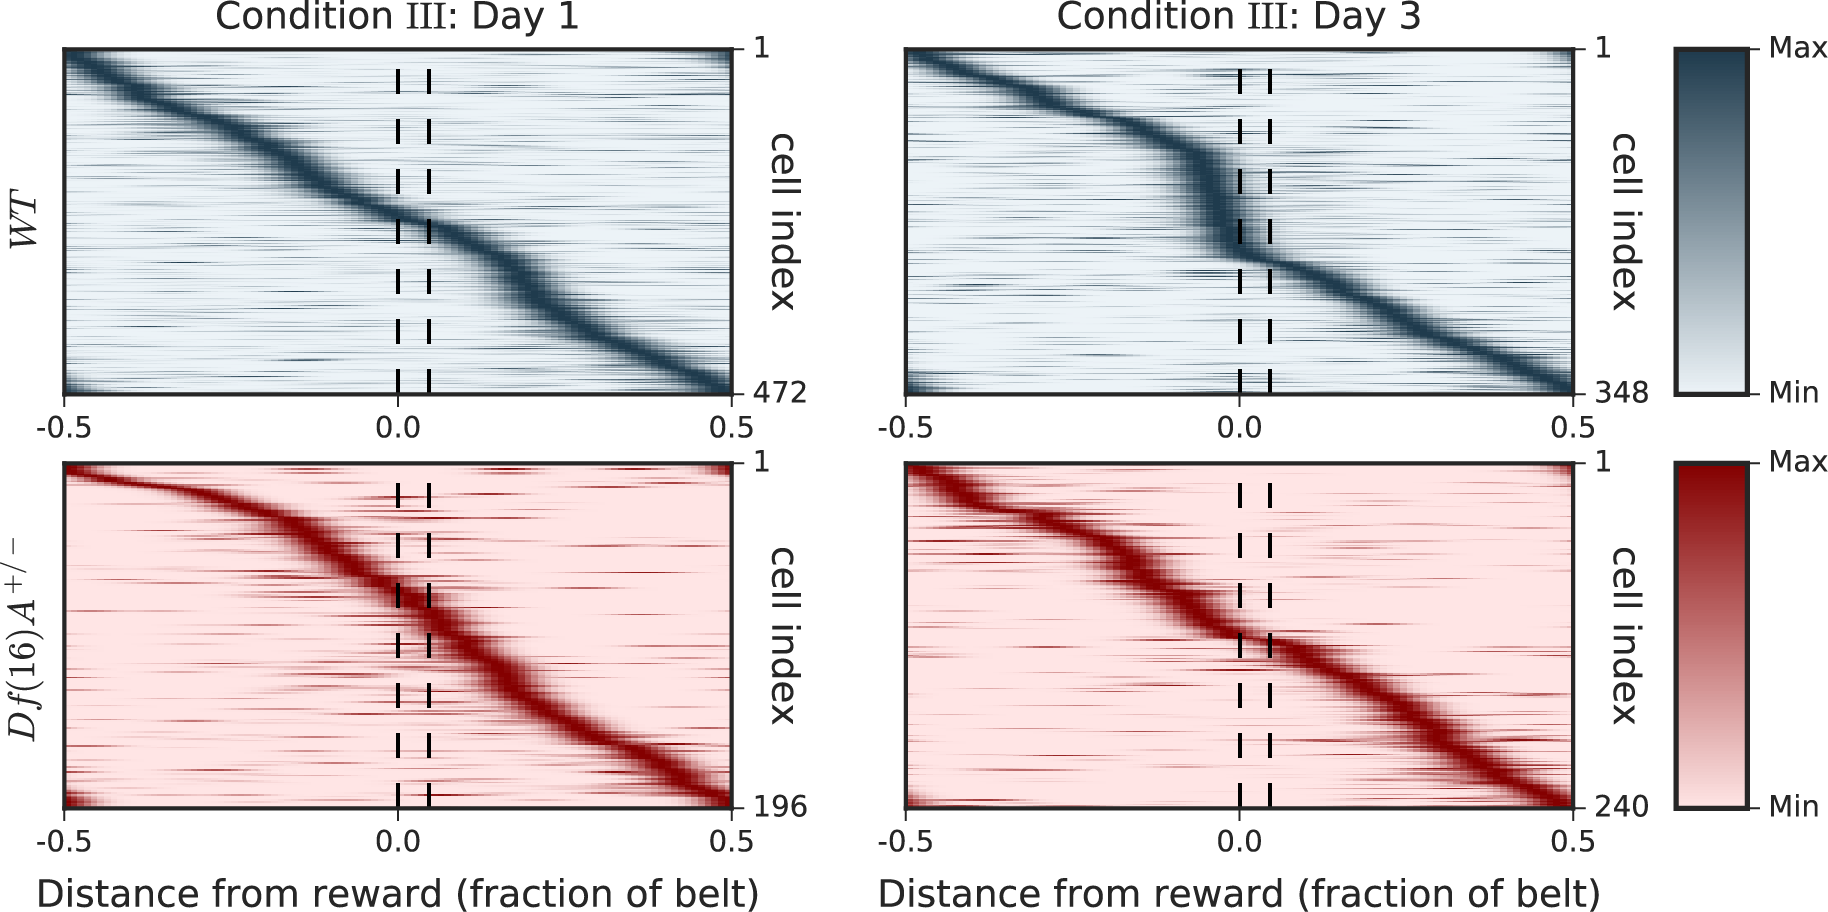
\includegraphics[width=0.7\textwidth]{df/Fig5_heatmaps}
	\caption[Heatmaps of place cell population throughout Condition~III]{Tuning profiles for all place cells in both WT and \df/ mice on the first and last day of Condition~III.
	Each row is an individual place cell. The intensity corresponds to the normalized transient rate in each spatial bin along the $x$-axis. Goal location is between dotted lines.
	WT mice show more place cells near the reward by day 3, an enrichment lacking in \df/ mice.}
	\label{fig:df:enrich_heatmaps}
\end{figure}

\begin{figure}
	\centering
	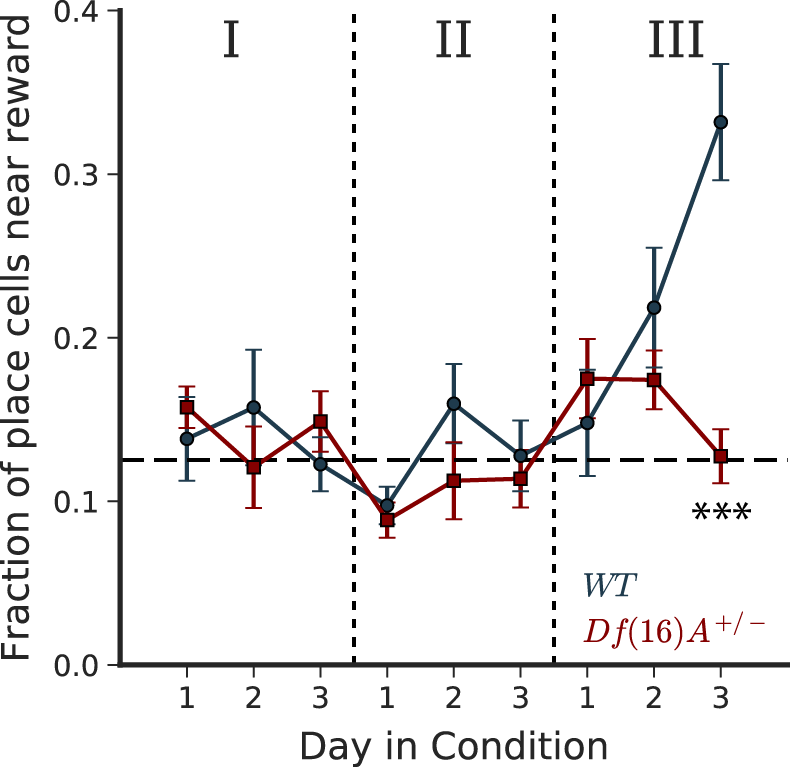
\includegraphics[width=0.5\textwidth]{df/Fig5_enrichment}
	\caption[Fraction of place cells near the goal location across all days of the experiment]{Fraction of place cells near the goal location (within $\frac{1}{16}$ of the belt length) across all days of the experiment.
	Dotted line is uniformly distributed fraction (two-way RM ANOVA: Genotype $\times$ Condition $\times$ Day interaction: F(4,124)=10.684, p$<$0.0001; Condition~I \& II: no significant effect of Genotype: F(1,31)=0.104, p=0.749 and F(1,31)=3.668, p=0.065; Condition~III: Genotype $\times$ Day interaction: F(2,62)=18.149, p$<$0.0001; main effect of Genotype: F(1,31)=12.051, p=0.002; post-hoc analysis with Bonferroni correction for multiple comparisons, Day 3: t=4.669, p=0.00017). ***p$<$0.001}
	\label{fig:df:enrichment}
\end{figure}

\begin{figure}
	\centering
	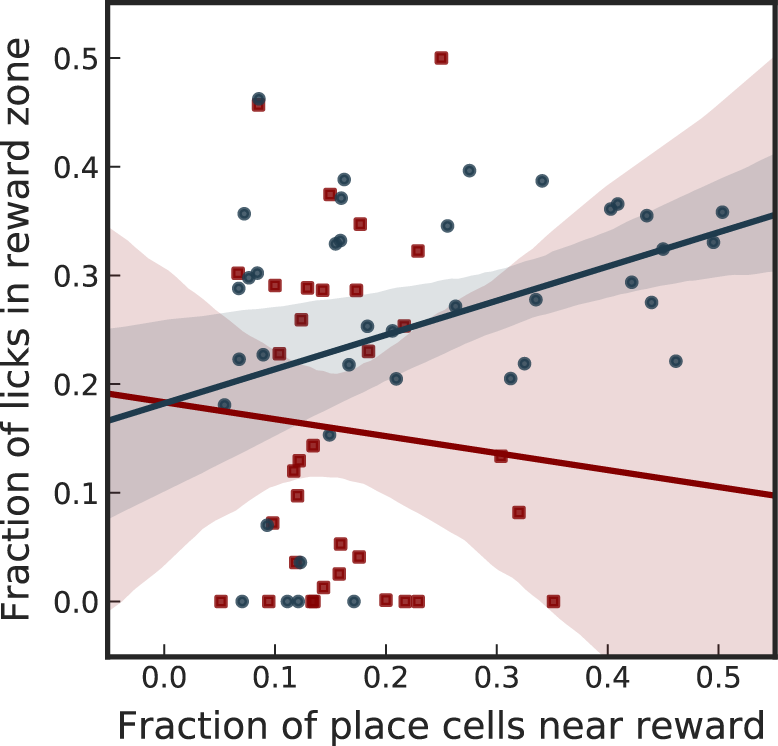
\includegraphics[width=0.5\textwidth]{df/Fig5_enrich_corr}
	\caption[Correlation of place cell goal-zone enrichment with task performance during Condition~III]{Place cell goal-zone enrichment correlation with task performance during Condition~III in WT, but not \df/, mice (WT: Pearson Correlation: 0.362, p=0.023; \df/: Pearson Correlation: -0.068, p=0.791). Linear regression and confidence intervals as in \autoref{fig:df:recurrence}c.}
	\label{fig:df:enrich_corr}
\end{figure}

\subsection{WT place fields shift towards the new reward location}
Several aspects of place cell population dynamics may explain the enrichment of firing fields at the goal location in the familiar context, for example: place cells within the reward zone may be more likely to recur as place cells with stable place fields; existing place fields may shift towards the reward \citep{Lee2006a}; or place fields at the reward location may be selectively stabilized compared to place fields farther away (Figures \ref{fig:df:remap_example} \& \ref{fig:df:possible_enrichment}).  In order to distinguish between these possibilities, we used WT mouse data from sessions during Condition~III to calculate the session-to-session place cell recurrence probability as well as the mean and variance of the place field centroid shift, as a function of the original place field's distance from the reward location (see \autoref{sec:df:methods:model}). We found a slight increase in recurrence probability of place cells that were active immediately preceding the reward (\autoref{fig:df:recurrence_fit}), though this effect is not strong enough to lead to reward location enrichment (see below). Interestingly, place fields drifted towards a location on the belt just after the reward zone, such that fields preceding it tended to shift forwards and fields following it tended to shift backwards (\autoref{fig:df:shift_fit}a,b). In addition, place fields just after the reward location shifted more consistently, as evidenced by a relatively lower place field shift variance (\autoref{fig:df:shift_fit}a,c). 

\begin{figure}
	\centering
	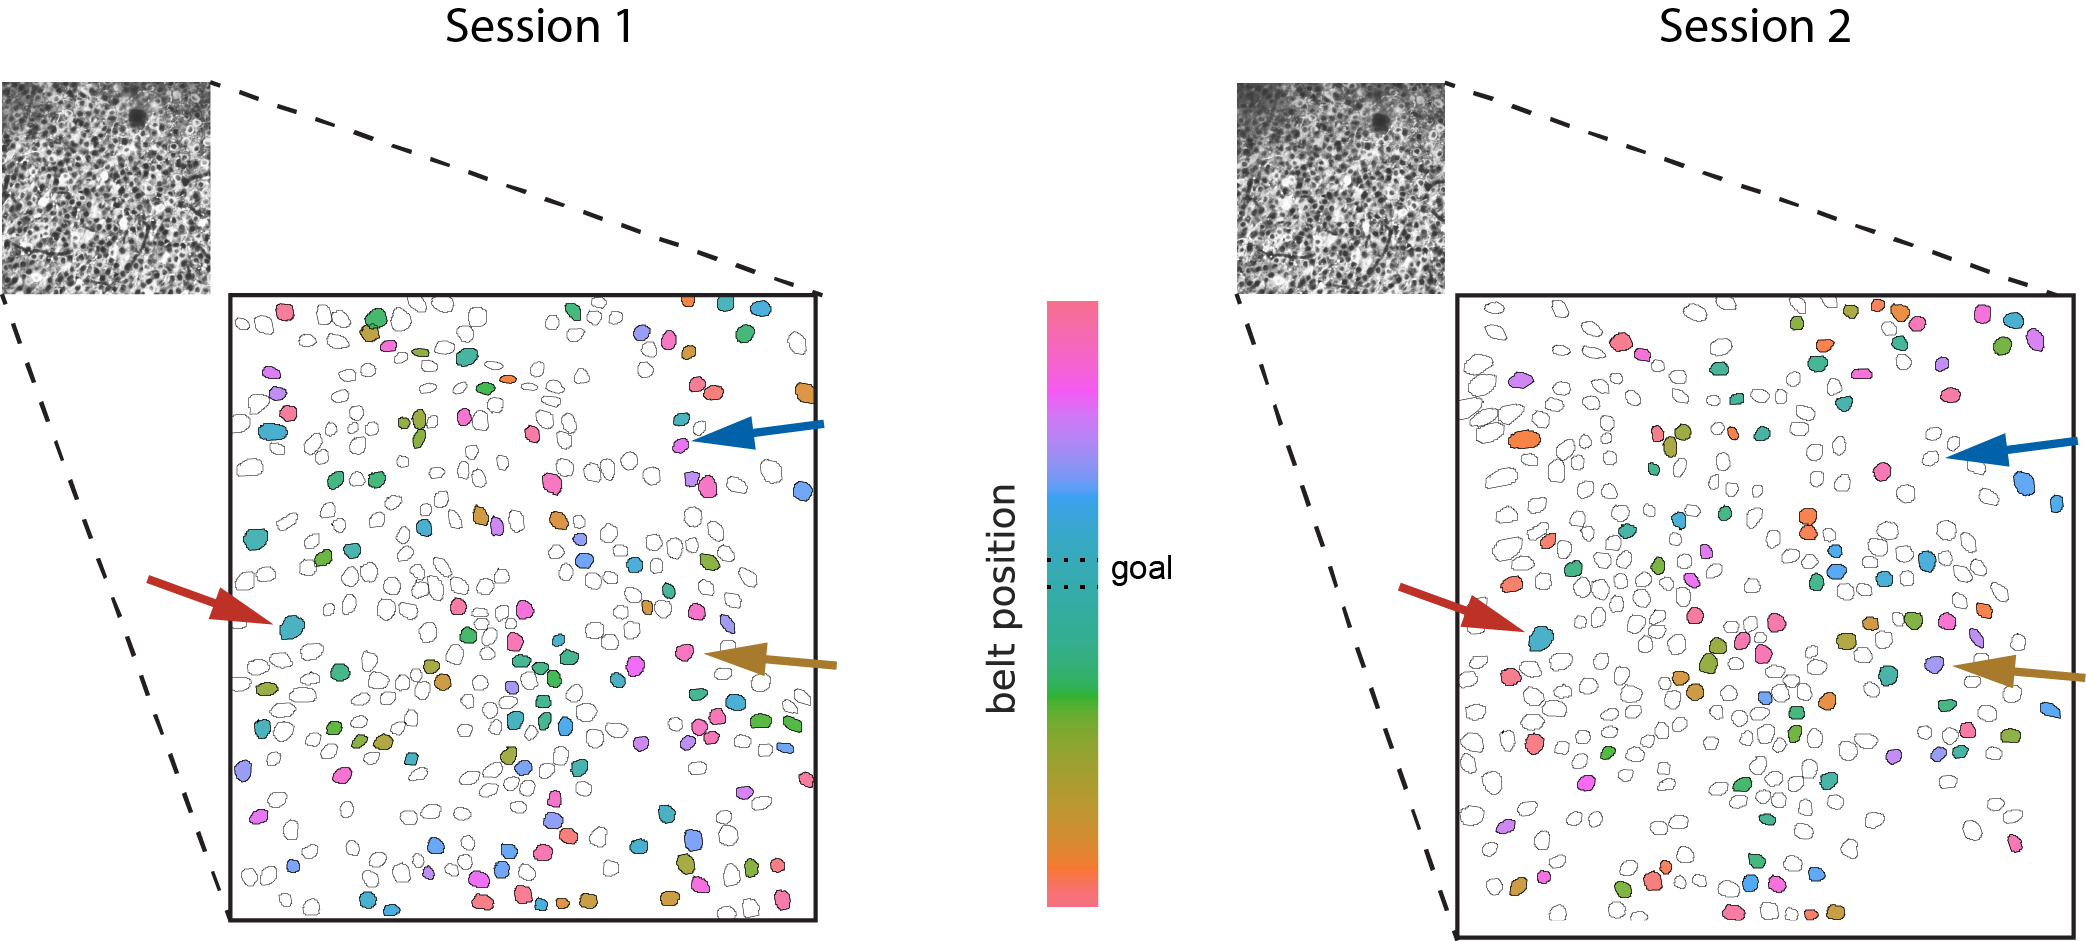
\includegraphics[width=0.9\textwidth]{df/Fig6_remap_example}
	\caption[Individual place field stability examples]{Example fields of view from two consecutive sessions. Background is time-averaged GCaMP6f movie. Place cells are colored corresponding to their spatial tuning within each session. The color bar shows the mapping of place field location on the belt. The reward zone for these sessions was between the dotted lines. Place fields are generally stable (red arrow), but some shift their place field (yellow arrow), while others stop being spatially active (blue arrow).}
	\label{fig:df:remap_example}
\end{figure}

\begin{figure}
	\centering
	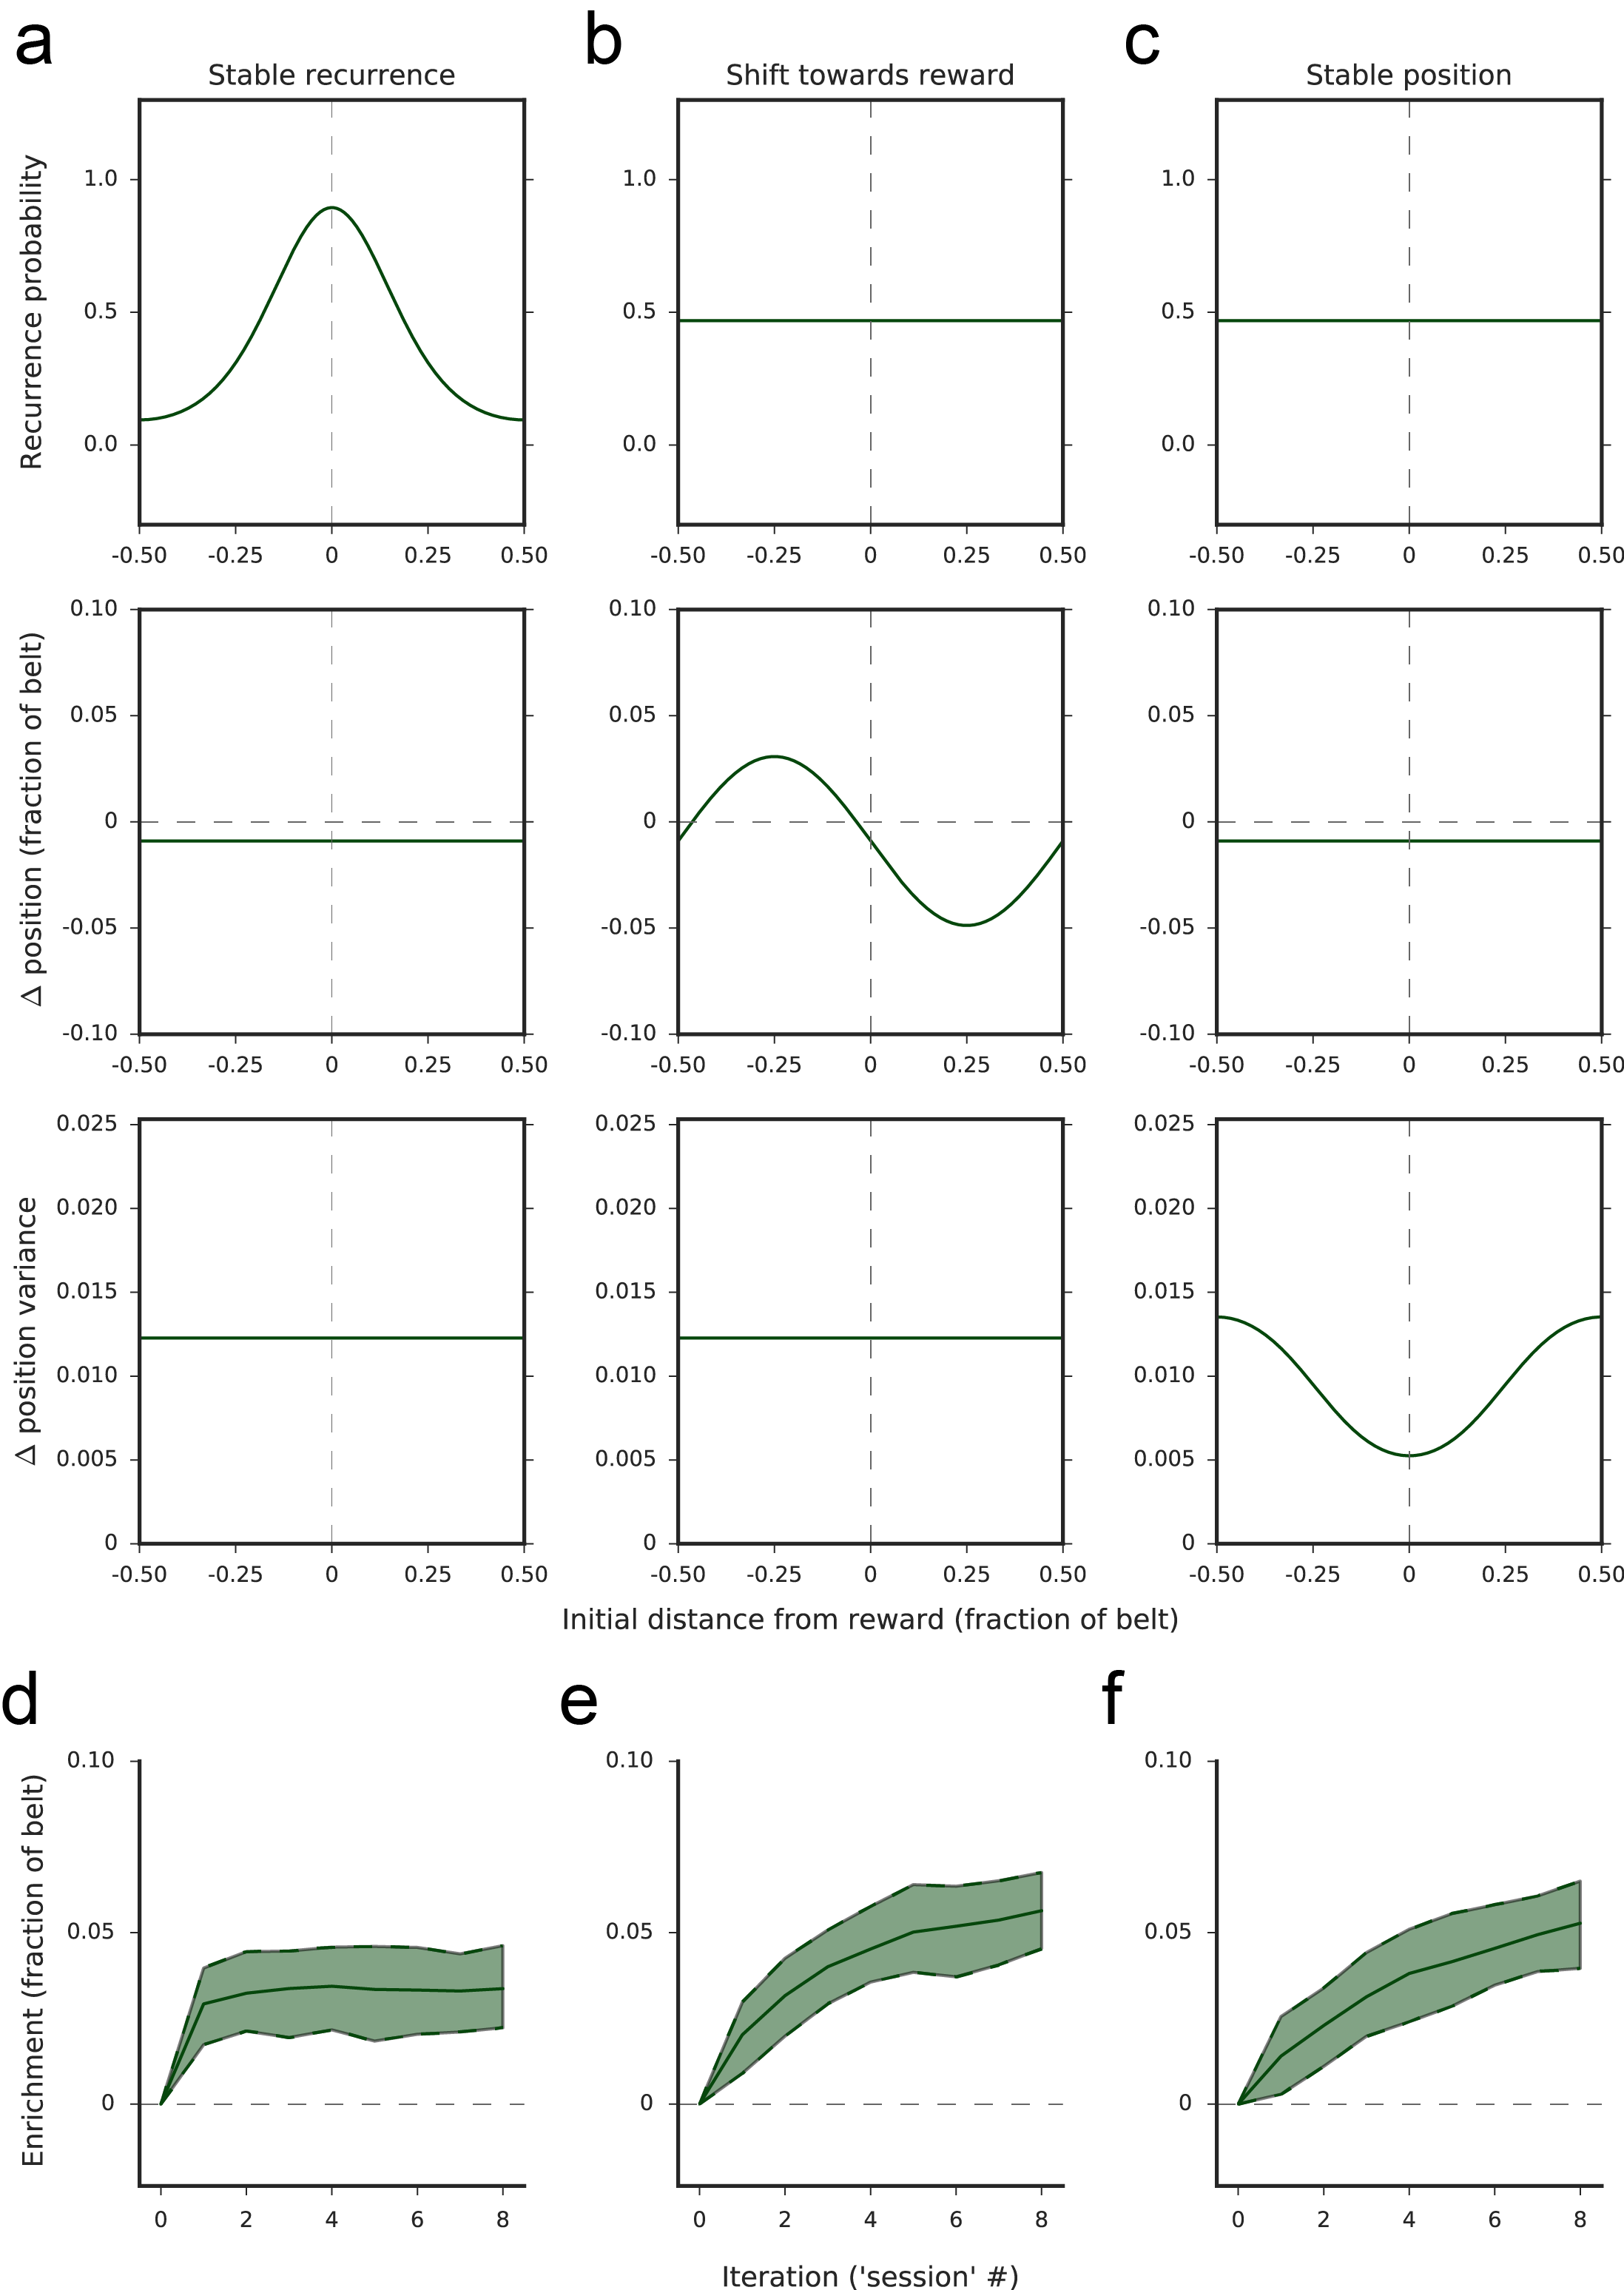
\includegraphics[width=0.7\textwidth]{df/FigS8_possible_enrichment_methods}
	\caption[Possible enrichment methods]{Comparison of three theoretical methods by which place cells could enrich a goal location.
	a. Place fields could be generally stable, but place cells near the reward are more likely to reoccur as place cells from session-to-session. (top) Recurrence probability as a function of distance from reward. (middle) Mean place field centroid shift as a function of distance from reward. (bottom) Mean place field shift variance as a function of distance from reward.
	b. Place cells could reoccur at equal probability along the belt, but place fields shift towards the reward location such that fields before the reward shift forward and fields after the reward shift backwards. Plots as in \emph{a}. Place fields shifting towards the reward also leads to enrichment in our model.
	c. Place fields might not shift uniformly towards the reward, but if fields are generally stable, the ones near the reward could shift less than ones farther away. Plots as in \emph{a}.
	d-f. Using the parameters from \emph{a-c}, our enrichment model suggests all three hypothetical models could lead to enrichments: (d) increased place cell recurrence at reward position, (e) place fields shifting towards the reward location, or (f) place fields near the reward shifting less than ones away from the reward.}
	\label{fig:df:possible_enrichment}
\end{figure}

\begin{figure}
	\centering
	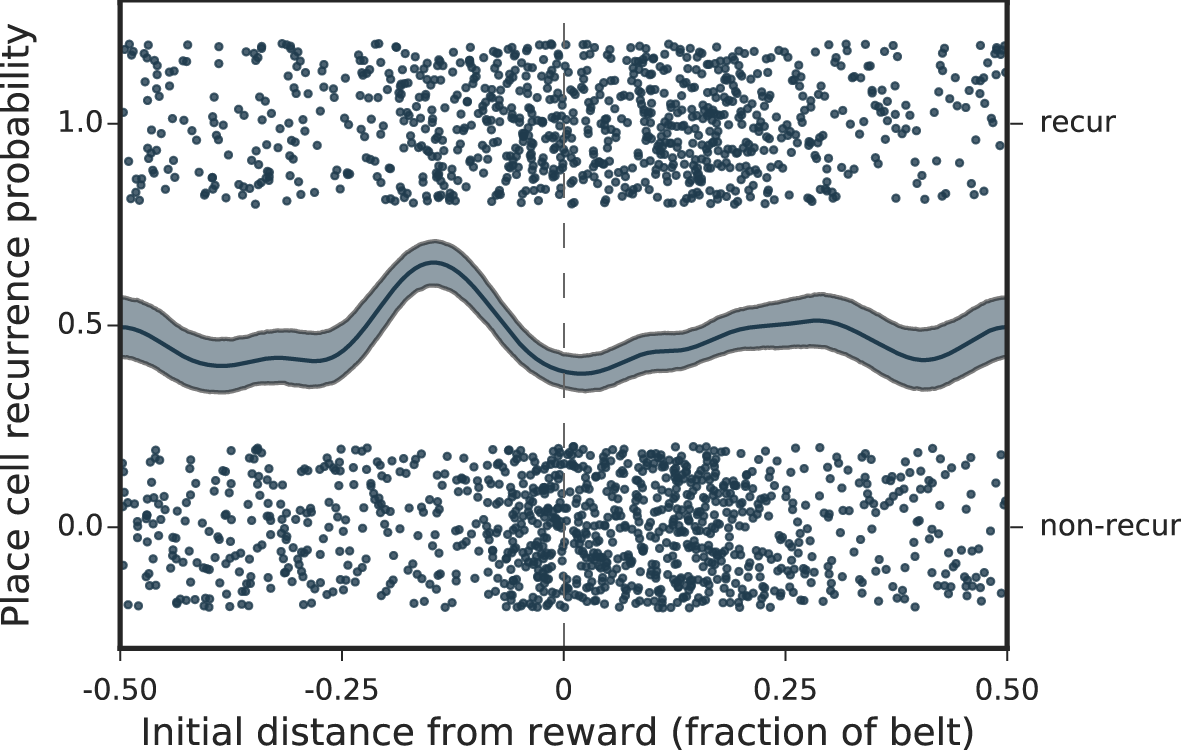
\includegraphics[width=0.5\textwidth]{df/Fig6_recurrence_fit}
	\caption[Recurrence probability as a function of original distance from the reward]{Recurrence probability as a function of original distance from the reward. For all pairs of consecutive sessions during Condition~III, each place cell during the first session is plotted with the centroid of its place field along the $x$-axis and whether or not it was also a place cell in the second session on the $y$-axis (top cluster is place cell in second session, bottom cluster is not a place cell, random $y$-axis jitter within each cluster for visualization). Cyclic logistic regression fit with 95\% confidence interval from cross-validation plotted on left axis.}
	\label{fig:df:recurrence_fit}
\end{figure}

\begin{figure}
	\centering
	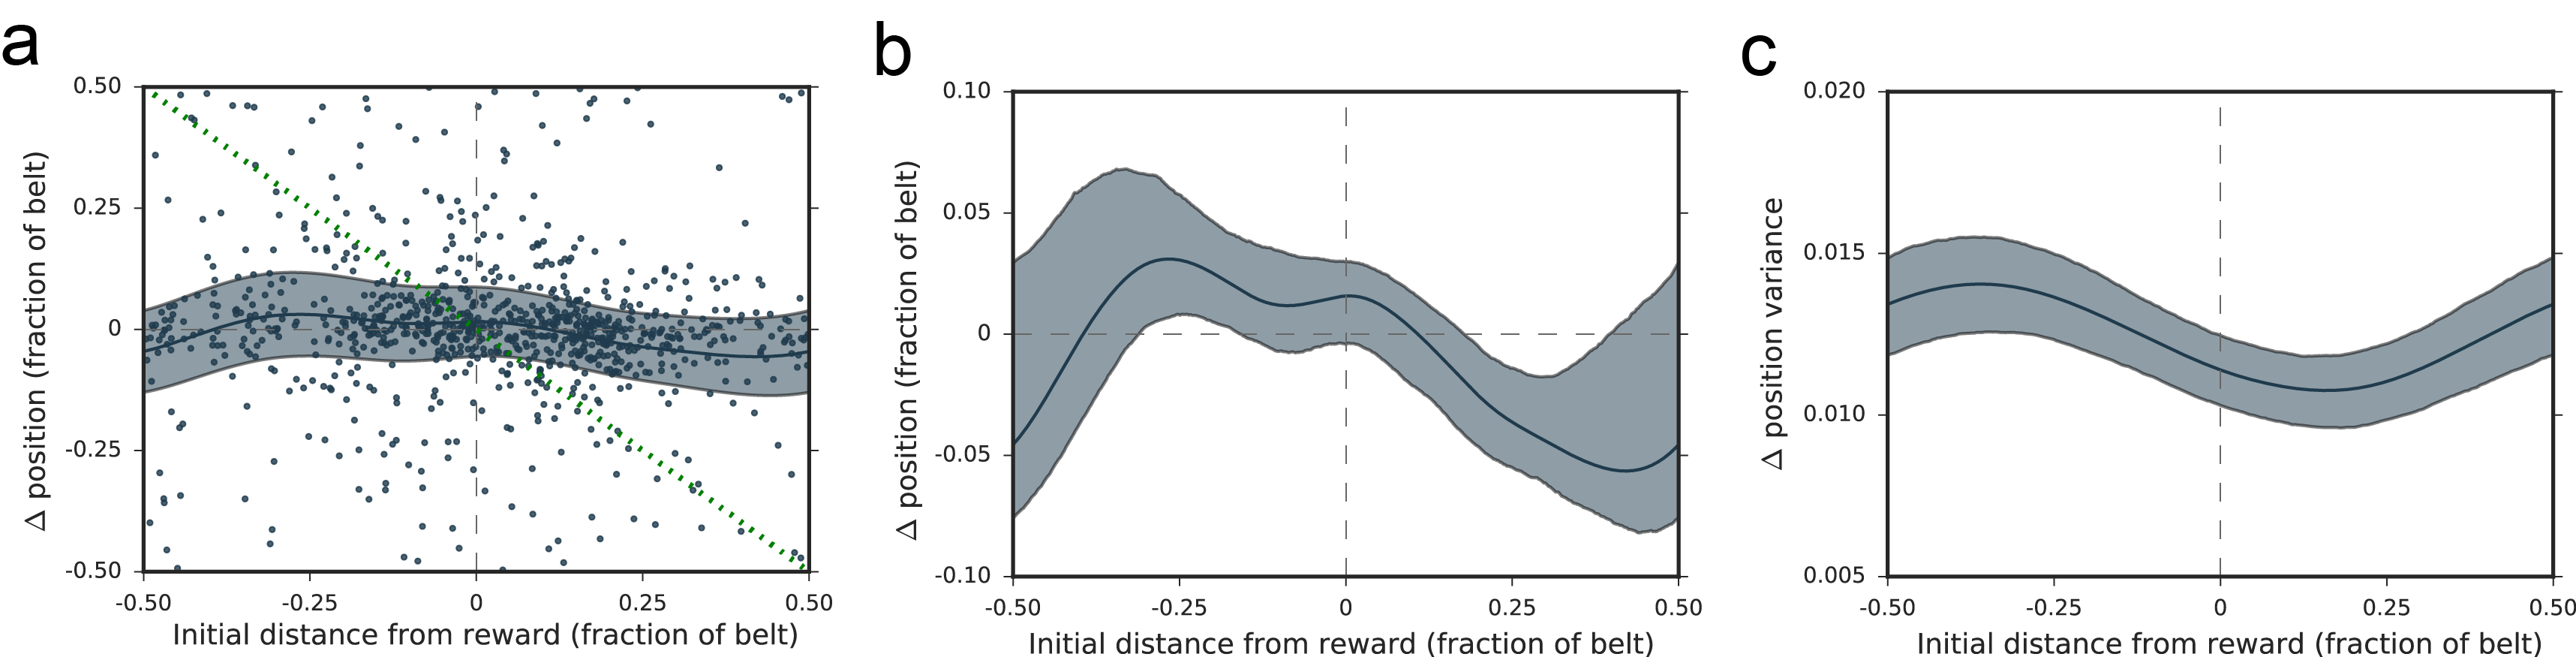
\includegraphics[width=0.9\textwidth]{df/Fig6_shift_fit}
	\caption[Session-to-session place field shift as a function of original distance from the reward]{a. Session-to-session place field shift as a function of original distance from the reward. For all pairs of consecutive sessions during Condition~III, each place cell during the first session is plotted with the centroid of its place field along the $x$-axis and the change in centroid position in the second session along the $y$-axis. Data is fit as a continuous series of von Mises distributions for each position, with the offset (solid line) and variance (shaded band, $\frac{1}{\kappa}$, where $\kappa$ is the concentration parameter) shown. Green dotted line denotes cells that move directly to the reward position in the second session.
	b. Same offset curve (solid line, shaded region is 90\% confidence interval calculated from refitting bootstrap resampled data) as in a. Positive values to the left of the zero-crossing and negative values to the right correspond to drift towards the reward position.
	c. Same variance fit as in a. (shaded region represents 90\% confidence interval calculated from refitting bootstrap resampled data) plotted independently. Place field shift is most consistent (minimum variance) at a position that corresponds to the most stable place field location from \emph{b}, just after the goal location.}
	\label{fig:df:shift_fit}
\end{figure}

\subsection{Modeling of place cell dynamics suggests that place fields shift is the primary factor leading to reward enrichment}
To determine the effect of these place fields stability properties on population-level spatial coding we next built a simple model of place cell stability and goal-oriented remapping. Our model assumes that every cell has a preferred spatial tuning each day, which is either latent (non-place cell) or expressed as significant spatial activity (place cell). This assumption is supported by the observation that even when a cell is not identified as a place cell, it retains a `memory' of the last time it was spatially active; firing closer to the old place field than expected by chance. Specifically, for all place cells from pairs of experiments separated by one session, the mean place field centroid shift variance between those two sessions was independent of the spatial information in the middle session (\autoref{fig:df:latent_tuning}).

\begin{figure}
	\centering
	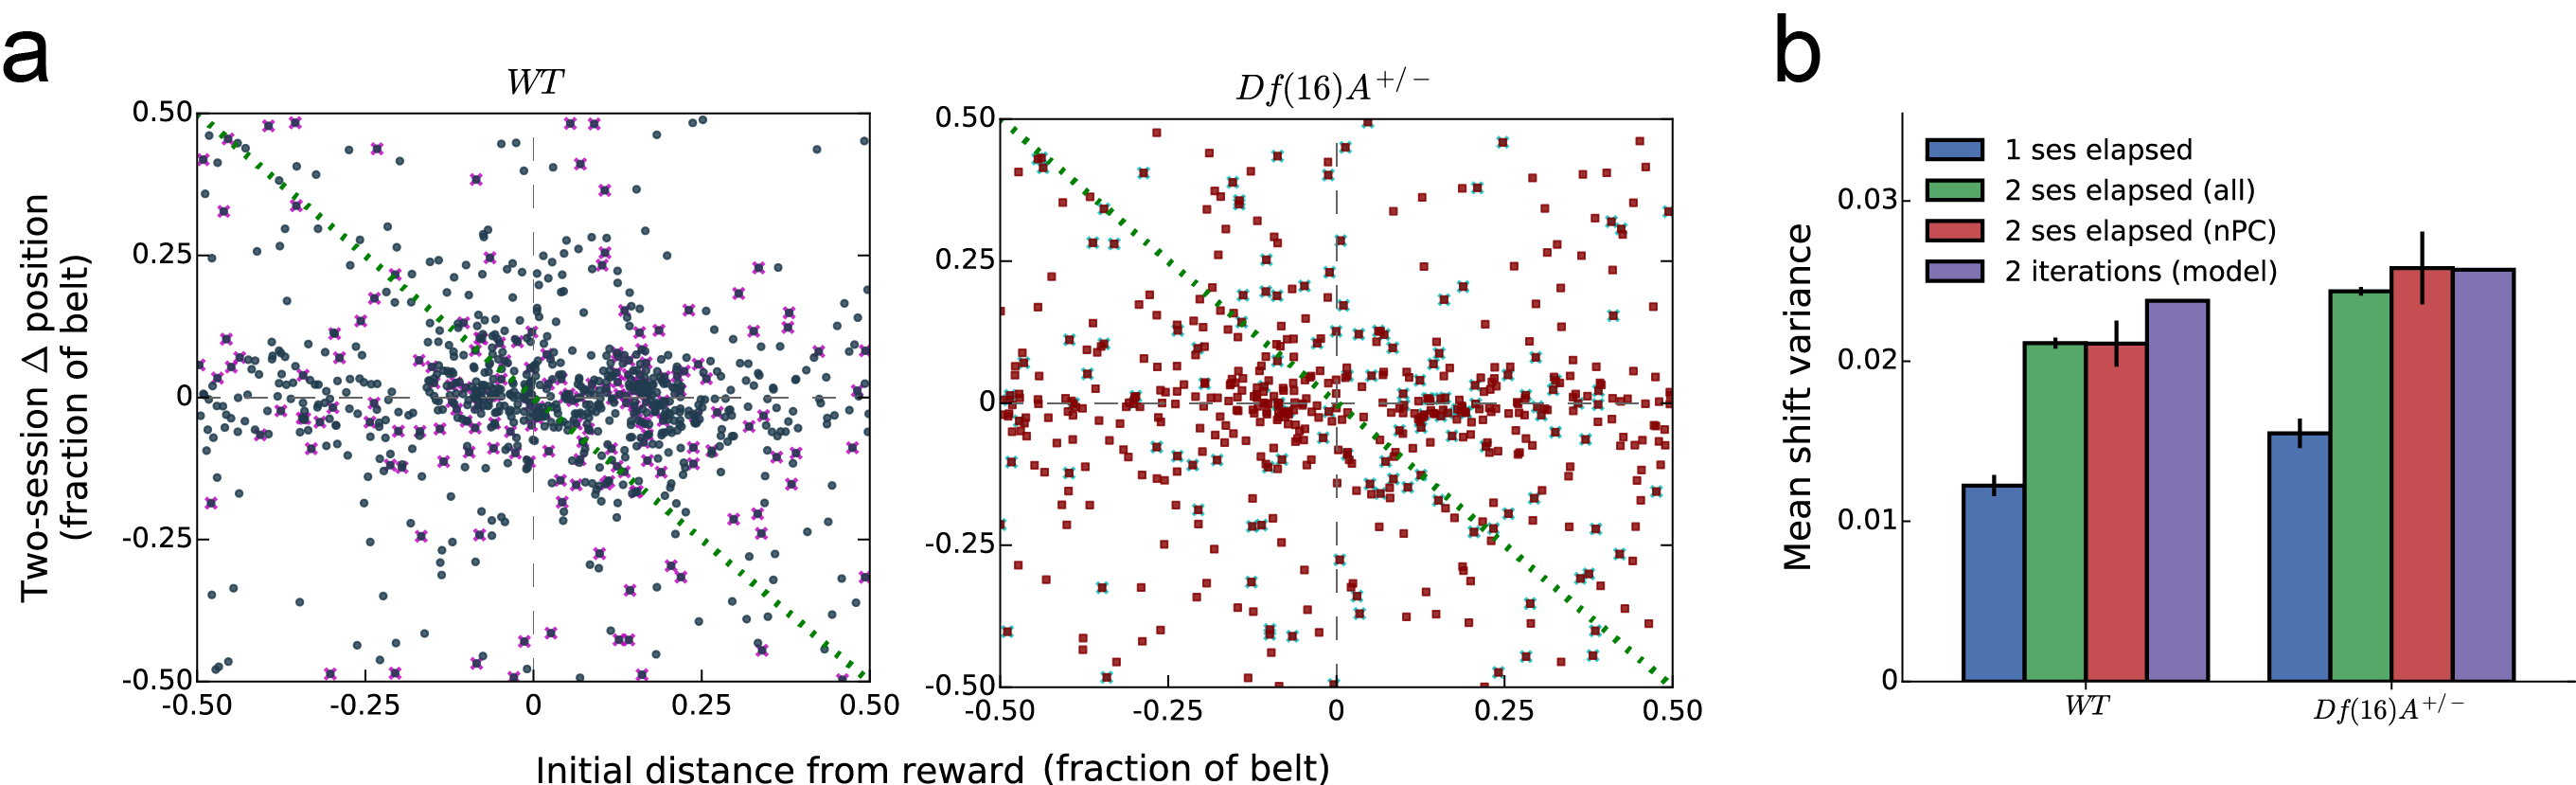
\includegraphics[width=0.9\textwidth]{df/FigS9_latent_tuning}
	\caption[Latent spatial tuning revealed across multiple sessions]{a. Scatter plots of original position versus position shift after 2 elapsed sessions for WT and \df/ mice. Cells that were not a place cell in the middle session are marked in magenta and cyan for WT and \df/ data, respectively. Even cells that were not a place cell in the intervening session still cluster around 0, suggesting that they retain some latent place preference that is either not expressed or not detectable. Vertical dashed line denotes reward location. Horizontal dashed line marks fields that do not shift at all. Green diagonal dashed line marks fields that remap directly to the reward location.
	b. Mean place field shift variance across all positions for cells paired by 1 session elapsed, 2 sessions elapsed, 2 sessions elapsed for cells that were not a place cell in the intervening session, and 2 iterations of the model. Two-session elapsed place cells are equally stable whether or not the cell was a place cell in the middle session, which is also the same as two iterations of the model.}
	\label{fig:df:latent_tuning}
\end{figure}

At each iteration (similar to 1 elapsed session) of the model (\autoref{fig:df:model_schematic}) non-place cells transition to place cells with a fixed probability calculated from the data ($P_{on}$) and place cells recur as place cells with the position-dependent recurrence probability calculated above ($P_{recur}(x_i)$, see \autoref{fig:df:recurrence_fit}). Additionally, all cells shift their preferred spatial tuning direction and the new firing position is randomly drawn from a von Mises distribution with position-dependent offset ($\mu(x_i)$, see \autoref{fig:df:shift_fit}b) and concentration ($\kappa(x_i)$, see \autoref{fig:df:shift_fit}c).

\begin{figure}
	\centering
	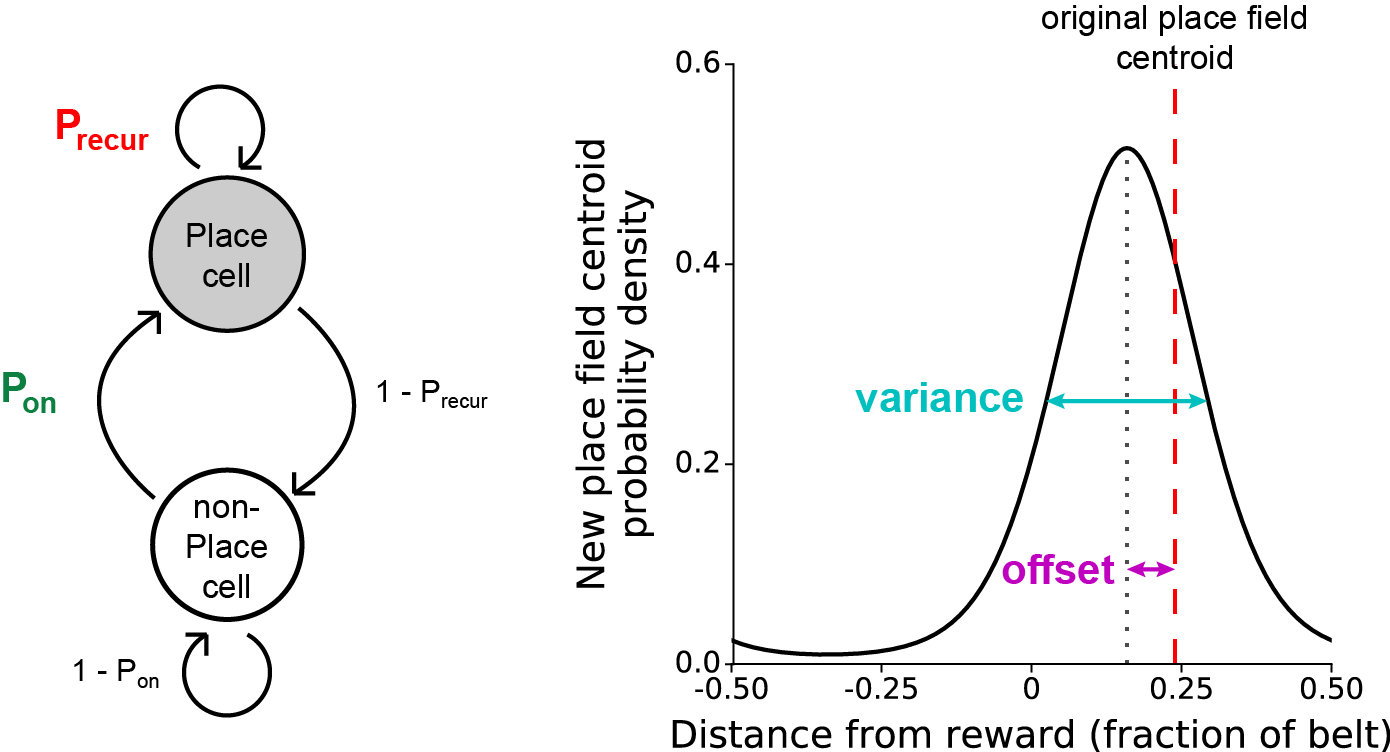
\includegraphics[width=0.7\textwidth]{df/Fig7_model_schematic}
	\caption[Place cell recurrence model schematic]{Schematic of place cell recurrence (left) and stability (right) model including the four parameters that were fit from our data: non-place cell-to-place cell transition probability ($P_{on}$), place cell recurrence probability by position ($P_{recur}$), session-to-session place field shift variance, and session-to-session place field shift offset.}
	\label{fig:df:model_schematic}
\end{figure}

By simulating the same number of session transitions as in our experimental paradigm we see the gradual enrichment of the goal location similar to the observed enrichment that we saw in the WT mice during Condition~III (\autoref{fig:df:model_results}). In contrast, when we fit the model from data taken from Condition~I or II, we do not see enrichment of the reward location, in agreement with the experimental data (\autoref{fig:df:model_all}). To asses which particular factor is driving goal enrichment, we created a \emph{flat} model for comparison by setting each of the position-dependent model parameters equal to the mean across all positions, effectively removing the dependence on the distance to reward by flattening out the fits, and as expected, with these parameters we do not see any enrichment (\autoref{fig:df:model_results}). We next swapped parameters one-by-one between our WT model and \emph{flat} model and re-ran the simulation, so as to see the effect of each parameter on the final goal enrichment. Flattening out either the recurrence probability or the place field shift variance resulted in very little change to the final level of place field enrichment with otherwise WT parameters. In contrast, by flattening out the place field shift, the population enrichment of the reward location completely disappeared (Figures \ref{fig:df:param_swap} \& \ref{fig:df:swap_supp}). In addition, if we take the \emph{flat} model and only replace the place field shift with the WT fit, we now see place field enrichment of the goal location (\autoref{fig:df:param_swap}a). We conclude that place field enrichment of goal locations is driven by an active recruitment of place fields shifting coherently towards the reward location.

\begin{figure}
	\centering
	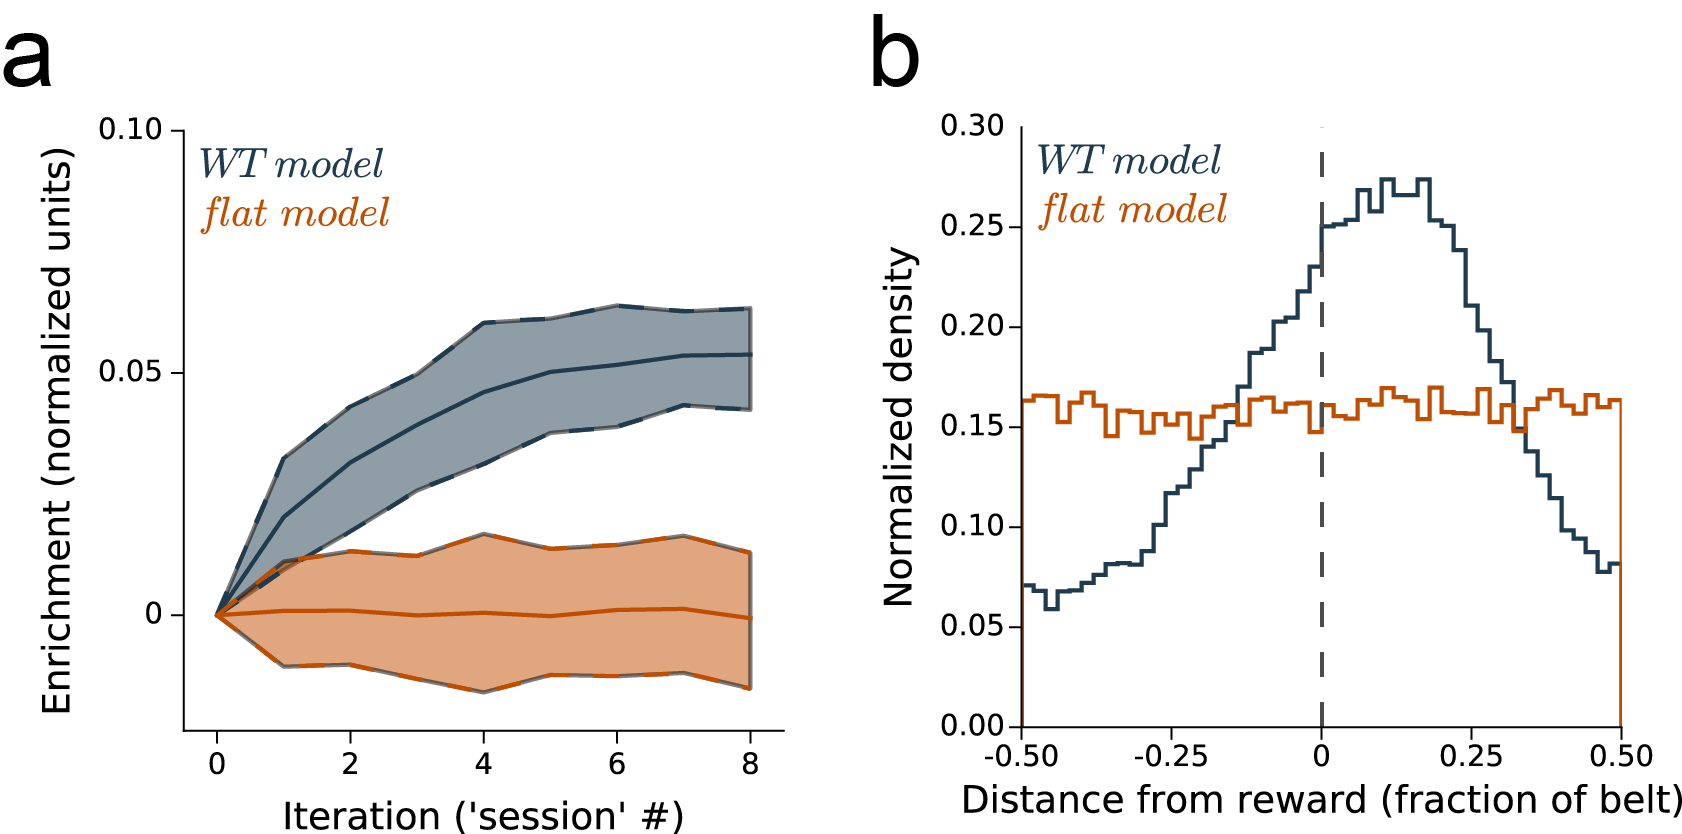
\includegraphics[width=0.7\textwidth]{df/Fig7_model_results}
	\caption[Simulated place field reward enrichment]{a. Mean population enrichment by simulated iteration for WT and \emph{flat} parameter sets ($\pm$~90\% confidence intervals from 100 simulations). WT parameters reproduce the enrichment observed during Condition~III.
	b. Final distribution of place fields after 8 iterations for WT and \emph{flat} parameters. Vertical dashed line denotes reward location.}
	\label{fig:df:model_results}
\end{figure}

\begin{figure}
	\centering
	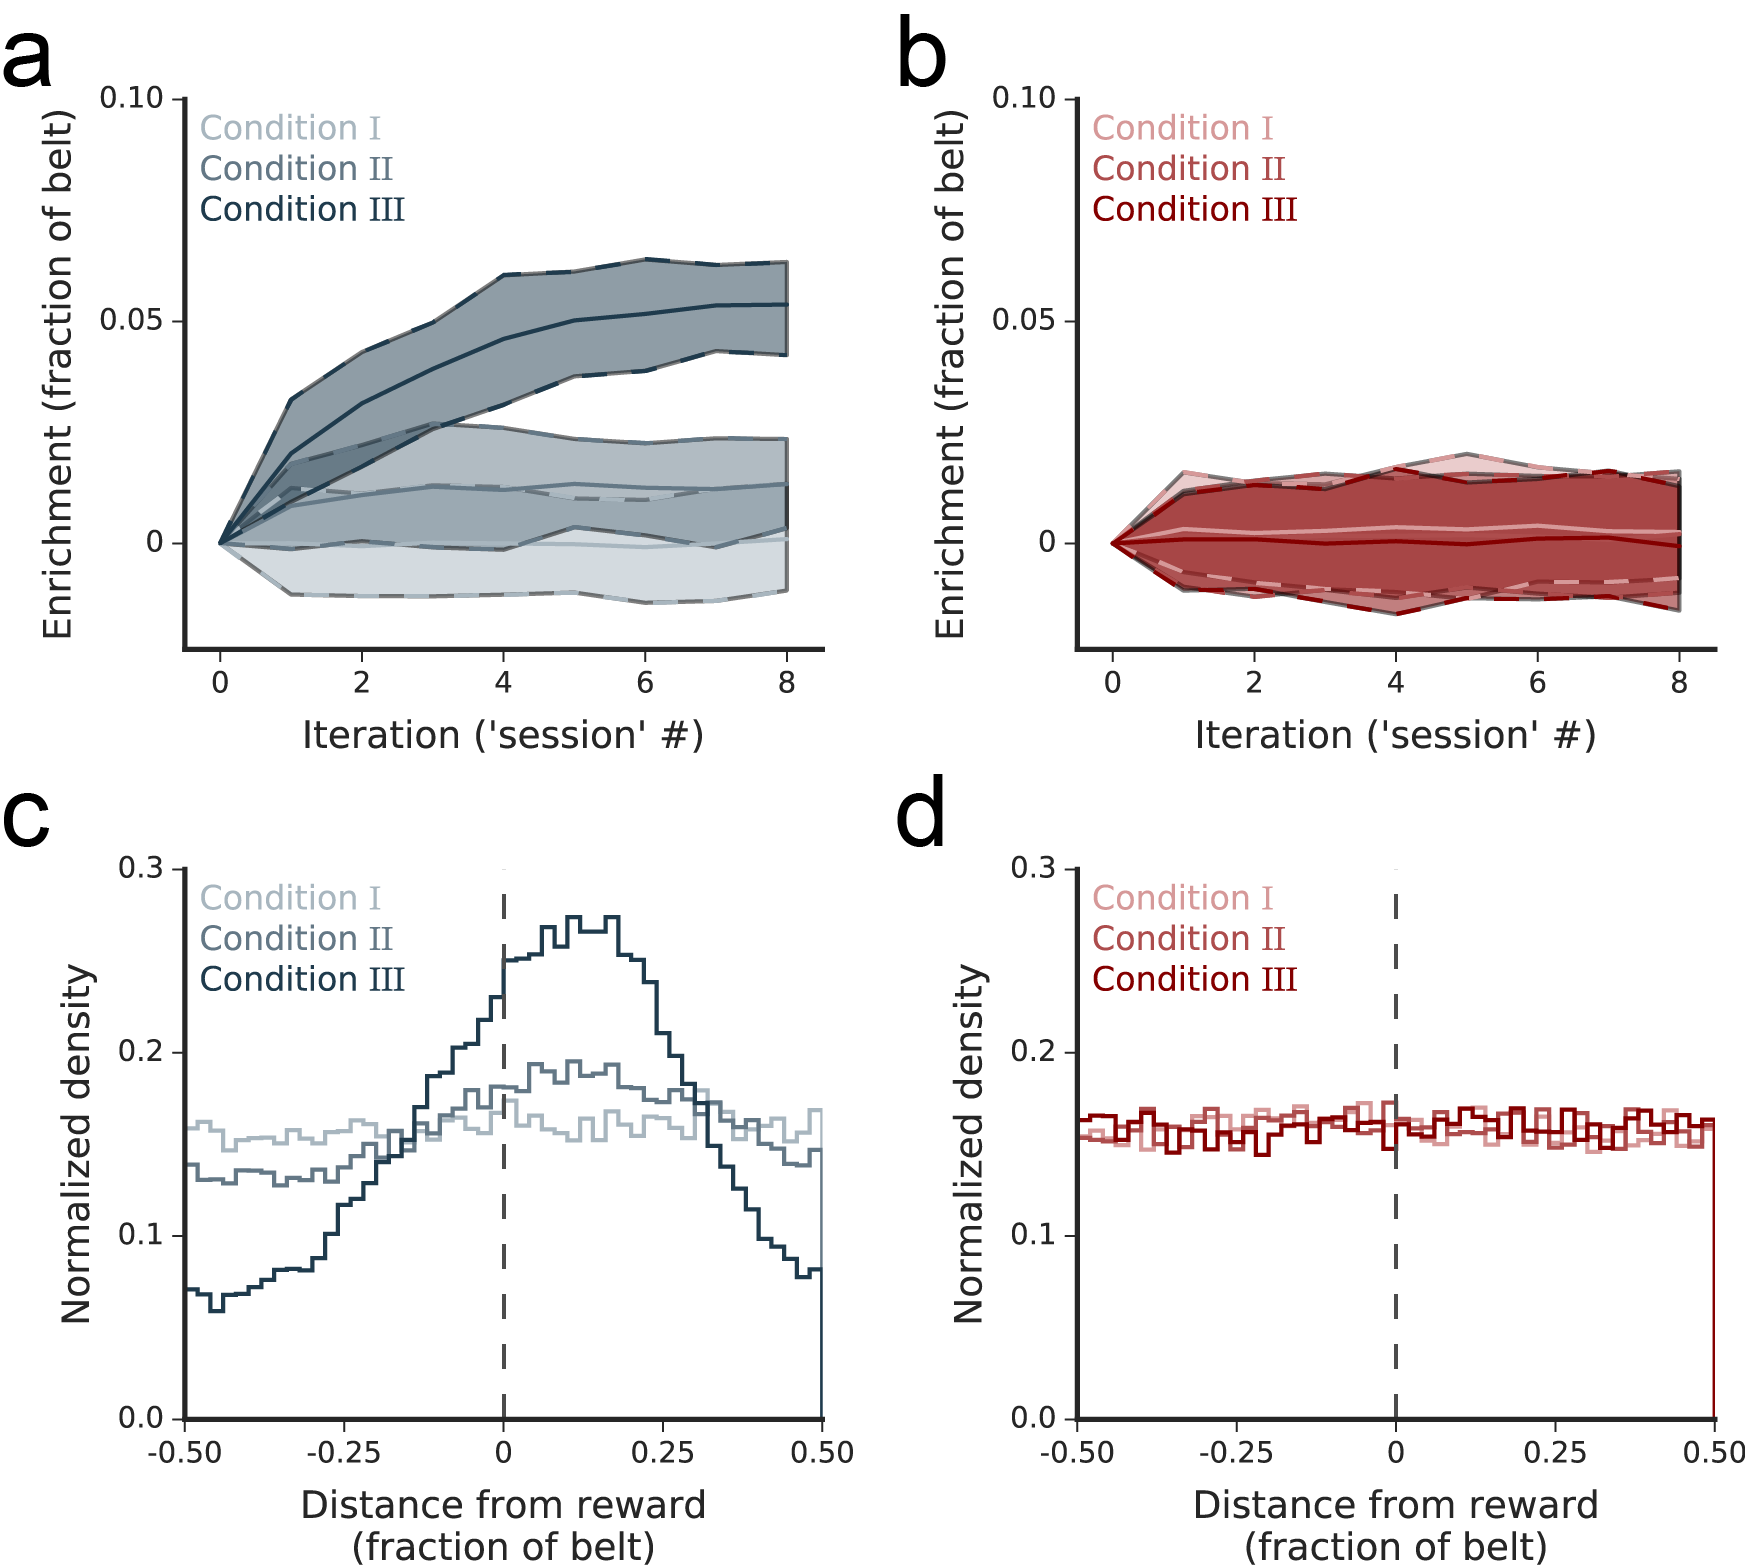
\includegraphics[width=0.7\textwidth]{df/FigS10_model_all_conditions}
	\caption[Modeled enrichment for all three Conditions]{Our model of place cell enrichment only produces goal location enrichment with parameters fit from WT mice during Condition~III.
	a,b. Enrichment by iteration with parameters fit from each of the three Conditions of the task for (a) WT and (b) \df/ mice (as in Figures \ref{fig:df:model_results}a \& \ref{fig:df:Df_model}e).
	c,d. Final distribution of place fields after 8 iterations for each set of parameters fit from (c) WT and (d) \df/ mice (as in Figures \ref{fig:df:model_results}b \& \ref{fig:df:Df_model}f).}
	\label{fig:df:model_all}
\end{figure}

\begin{figure}
	\centering
	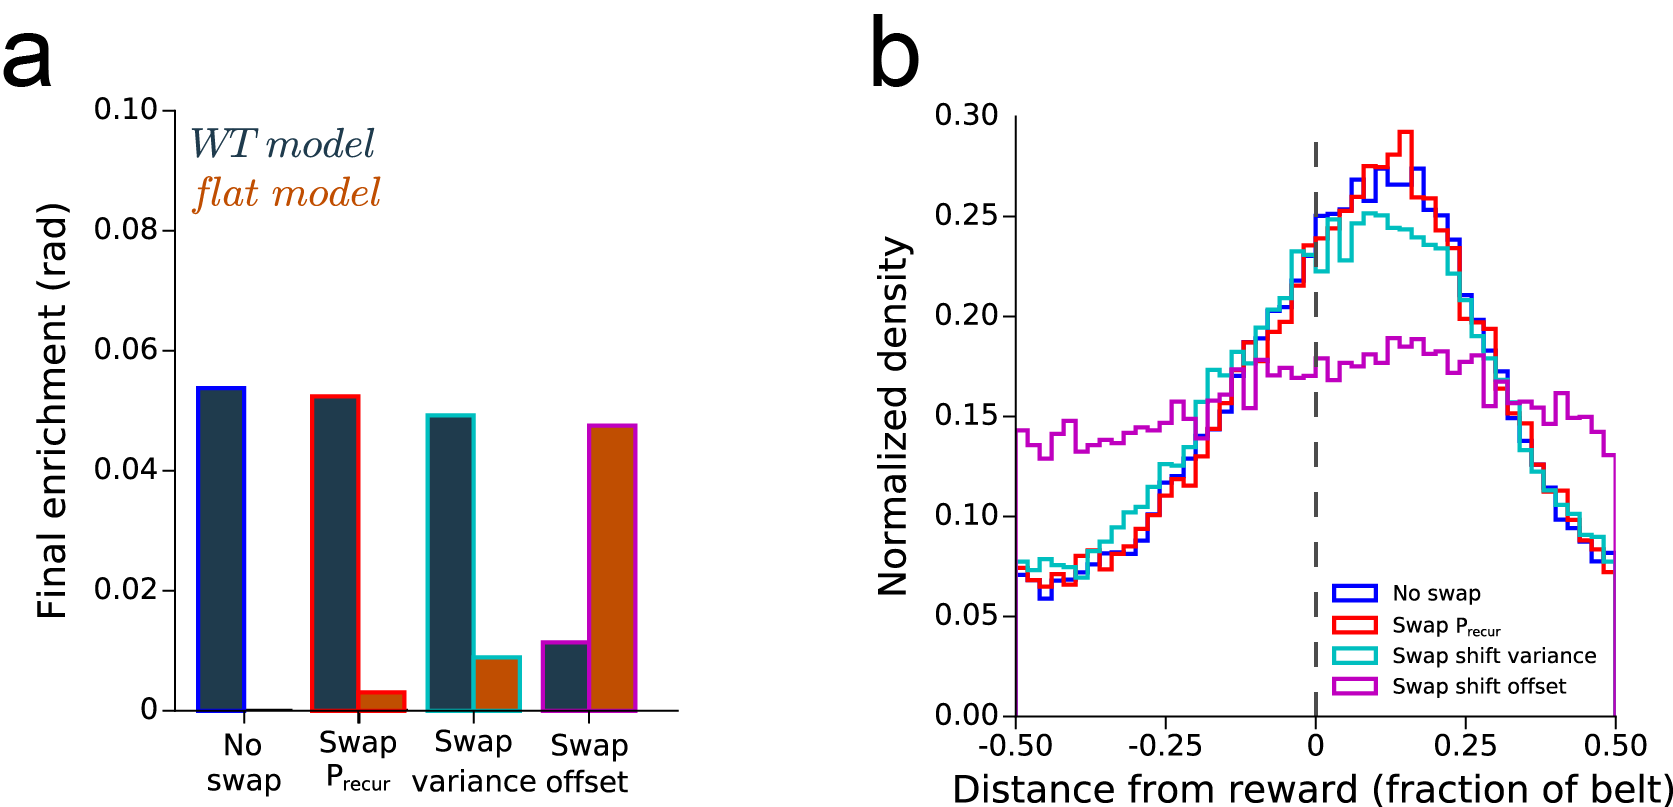
\includegraphics[width=0.7\textwidth]{df/Fig7_param_swap}
	\caption[Place field shift towards the reward drives reward enrichment in model]{a. Mean population enrichment after 8 iterations with true fit parameters and then swapping each set of position-dependent parameters individually between WT and \emph{flat}: recurrence probability ($P_{recur}$), place field shift variance, and place field shift offset.
	b. Final WT place field distributions after 8 iterations with the same parameter swaps as in \emph{a}. Mean place field shift (offset) toward the reward is revealed as the main factor underlying enrichment in GOL.}
	\label{fig:df:param_swap}
\end{figure}

\begin{figure}
	\centering
	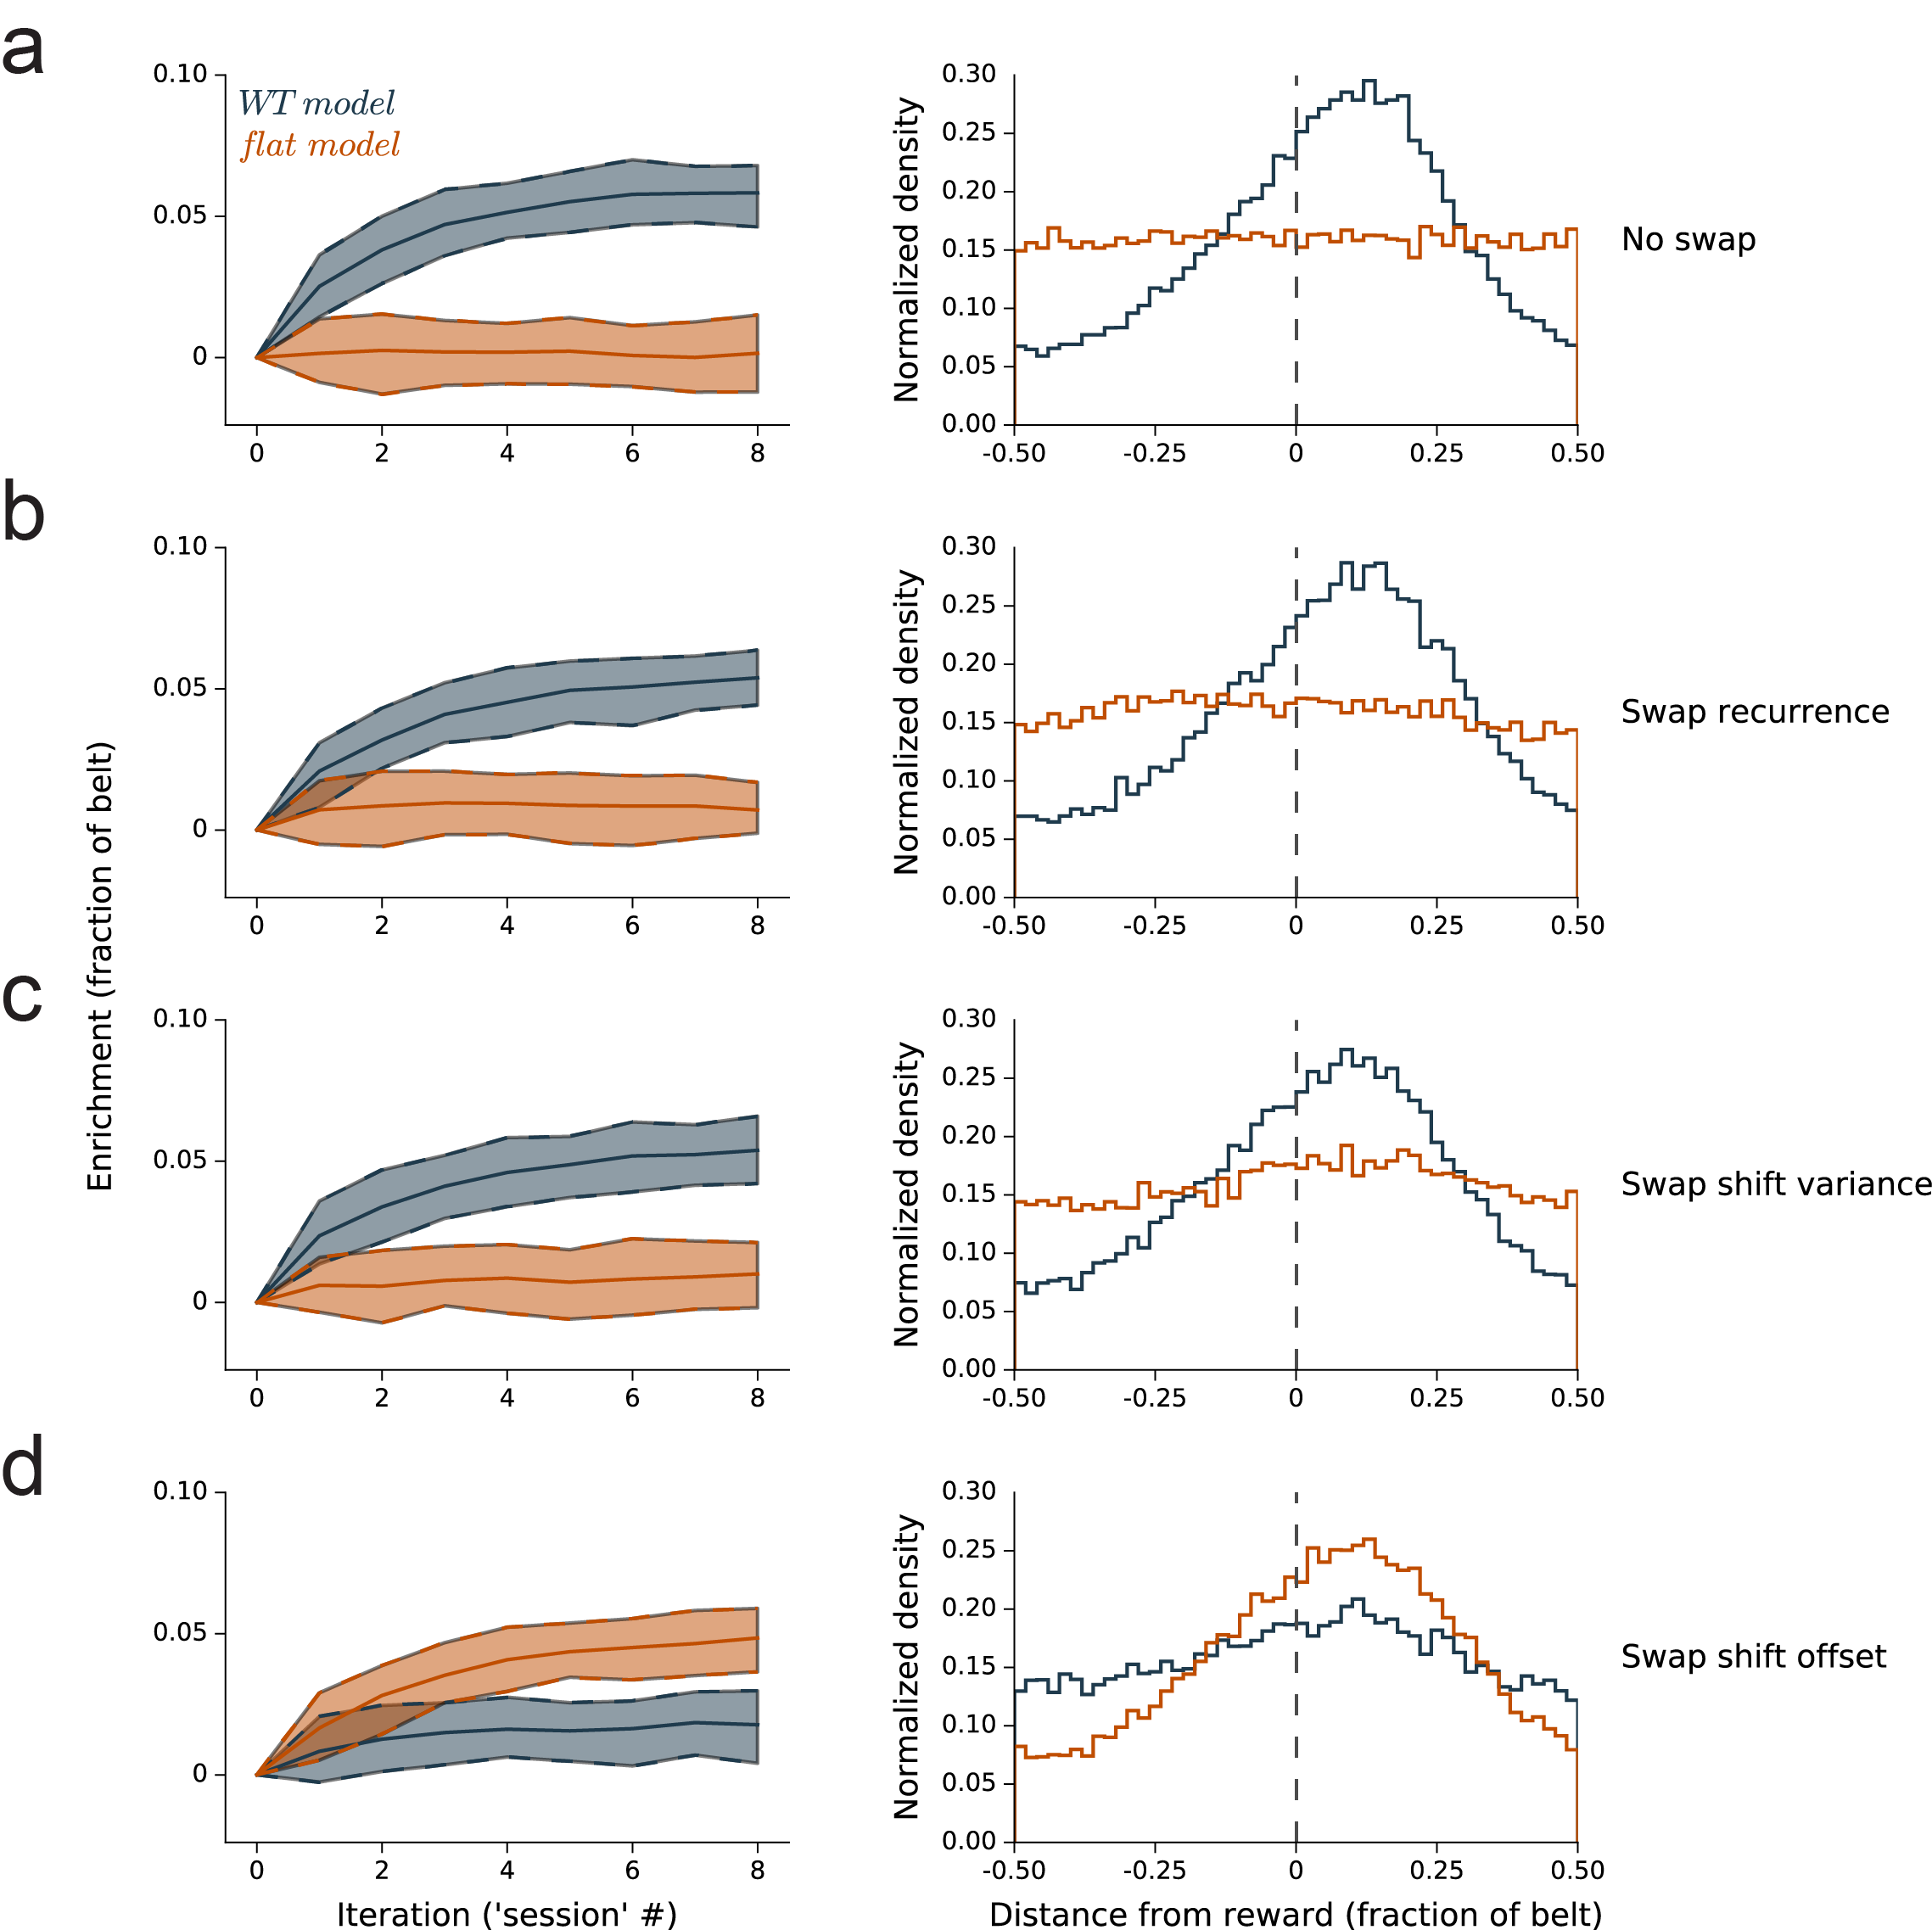
\includegraphics[width=0.8\textwidth]{df/FigS11_model_swap_parameters}
	\caption[Model enrichment when swapping individual parameters between WT and \df/ values]{Mean enrichment by iteration (left, 90\% confidence interval shading determined from 100 simulations) and histogram of distributions of place fields after the final iteration (right, data pooled across all simulations, vertical dashed line denotes reward location) for each parameter individually swapped between WT and \emph{flat} models.
	a. No swap.
	b. Swap place cell recurrence probability ($P_{recur}$).
	c. Swap session-to-session place field shift variance.
	d. Swap session-to-session place field shift offset. Swapping shift offset has the largest effect, as the \emph{flat} model with only the WT shift offset parameters leads to enrichment, while the WT model with the \emph{flat} shift offset parameters does not.}
	\label{fig:df:swap_supp}
\end{figure}

\subsection{Modeling of place cell dynamics corroborates the absence of enrichment in the \df/ mice through lack of place field shift towards reward}
While we saw robust place field enrichment of the reward location in WT mice following a change in the reward location, population enrichment was completely absent in \df/ mice. In order to gain insight into the lack of enrichment, we calculated the recurrence probability, place field shift, and place field shift variance as a function of distance from reward during Condition~III with the \df/ data, as we did with the WT data. All three parameters show no dependence on position for the recurrence probability, place field shift, or the place field shift variance (\autoref{fig:df:Df_model}a-d). Consistent with previous studies \citep{Mehta1997} across the entire belt on average place fields shifted slightly backwards (\autoref{fig:df:Df_model}c) and when we simulated session-to-session place field shifts with our model we do not see any enrichment of the goal location (\autoref{fig:df:Df_model}e,f). We conclude that while WT place fields shift toward the reward location, leading to an over-representation of this location, this effect is disrupted in \df/ mice.

\begin{figure}
	\centering
	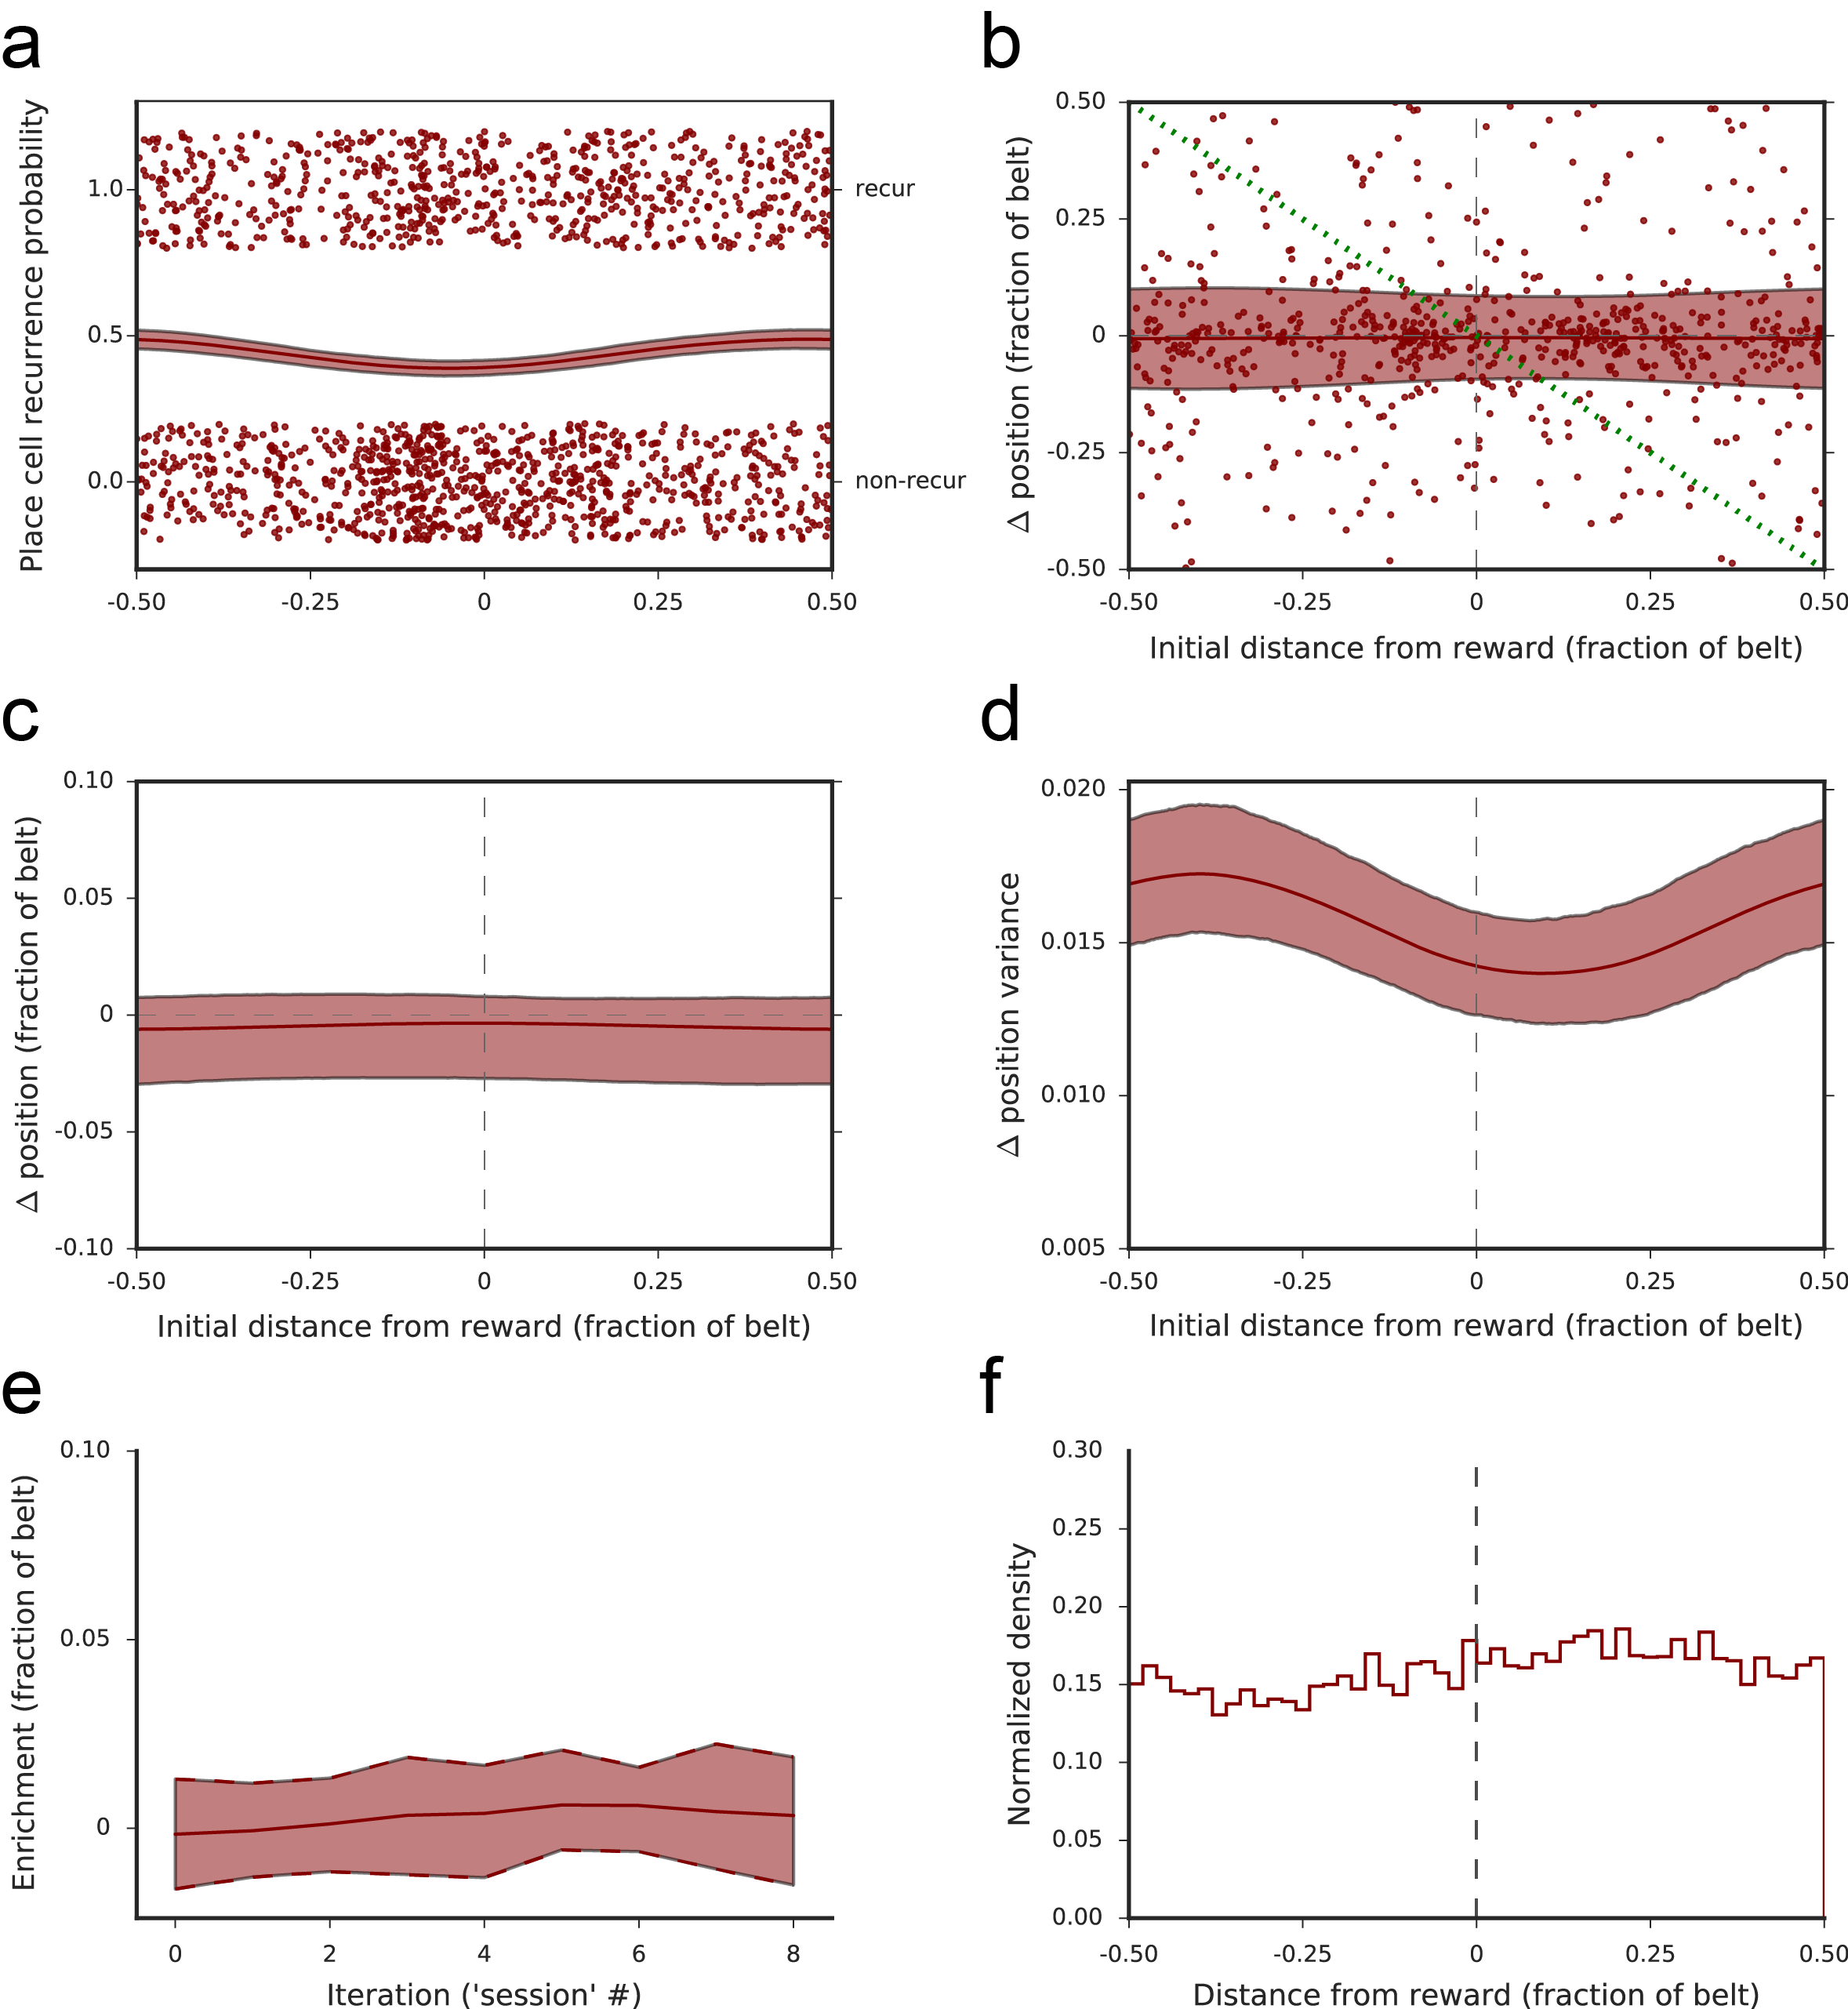
\includegraphics[width=0.8\textwidth]{df/Fig8_Df_model}
	\caption[\df/ mice place fields do not drift towards goal and model produces no enrichment]{a. Place cell recurrence by distance from reward as in \autoref{fig:df:recurrence_fit}.
	b. Session-to-session place field shift as a function of original distance from the reward as in \autoref{fig:df:shift_fit}a.
	c,d. Place field shift and variance fits from \emph{b} as in \autoref{fig:df:shift_fit}b,c (shaded region is 90\% confidence interval calculated from refitting bootstrap resampled data).
	e. Unlike WT model, enrichment model with \df/ parameters shows no enrichment (see \autoref{fig:df:model_results}a).
	f. Final distribution of place fields after 8 iterations for \df/ parameters.}
	\label{fig:df:Df_model}
\end{figure}

\section{Discussion}

Our study provides the first comparative characterization of learning-related neural population dynamics in the hippocampus with chronic cellular-resolution functional imaging in wild-type and mutant mice carrying a SCZ-predisposing genetic lesion. We found that mice carrying the 22q11.2 deletion, one of the strongest genetic risk factors for cognitive dysfunction and SCZ, exhibit compromised stability and plasticity of hippocampal place cell maps during spatially guided reward learning. Broadly interpreted, our results provide further insight into the normal roles of neuronal ensemble stability and plastic reorganization under specific learning conditions. Further, we show that genetic mutations predisposing to neuropsychiatric and cognitive disorders can lead to learning deficits through disruptions in these fundamental features of hippocampal population dynamics. 

\subsection{Hippocampal place cell dynamics depend on both the task and the specific task parameters in goal-directed learning}

Long-term stability of hippocampal spatial representation is a widely posited prerequisite for reliable spatial learning \citep{Kentros2004, Lever2002b, Mankin2012, Thompson1990, Ziv2013}. By tracking hippocampal place cell dynamics over different phases of a multiday learning task, our study extends previous findings by showing a positive correlation between place cell map stability and learning performance in both WT and \df/ mice (see Figures \ref{fig:df:recurrence}c, \ref{fig:df:cent_shift}c, \& \ref{fig:df:pf_corr}c). Indeed, task performance and spatial map stability for each genotype followed a similar trajectory as task demands changed; more specifically, task performance and stability were most similar during Condition~I, \df/ mice were slightly impaired in Condition~II, and the largest difference was observed in Condition~III (see \autoref{fig:df:trajectories}). These findings strongly suggest that the neural coding strategy employed during all phases of a spatial reward learning task relies on the formation and maintenance of stable hippocampal representations, both in terms of place cell identity and place field location. Our results also show task-dependent stabilization of spatial maps in WT mice, as WT place fields were significantly more stable in the GOL task than during random foraging, an effect possibly mediated by the attentional demands of GOL \citep{Kentros2004, Kobayashi1997, Markus1995, Monaco2014}. In contrast, place field stability between GOL and RF tasks was indistinguishable in \df/ mice, indicative of a failure to conditionally stabilize spatial maps instrumental in finding rewarded locations (see \autoref{fig:df:RF}c). However, \df/ mice were comparable to WT littermates in their ability to initially learn a reward location, as well as in baseline place cell stability, which suggests that the \df/ learning deficit was related to the stabilization and rearrangement of spatial maps in response to changing task demands (Condition~I, see Figures \ref{fig:df:licktograms}, \ref{fig:df:task_performance}, \& \ref{fig:df:trajectories}).

Our results also suggest that the memory deficit throughout the GOL task may result from impaired consolidation processes. \df/ mice were capable of solving this task, but they were significantly impaired at the beginning of each day (\autoref{fig:df:performance_by_session_in_day}) and spatial maps are significantly less stable overnight, compared to the WT mice (Figures \ref{fig:df:recurrence}b, \ref{fig:df:cent_shift}b, \& \ref{fig:df:pf_corr}b). In that respect, the altered SWR activity we observe in the \df/ mice may underlie the decreased stability of spatial maps.  SWRs are thought to support reactivation and consolidation of memories of previous experiences and planned future experiences \citep{Buzsaki2015, Diba2007, Foster2006, Jadhav2012, Kudrimoti1999}, and the strength of SWR-related reactivation has been shown to correlate with subsequent memory expression \citep{Dupret2010a}. Although we did not directly asses place cell reactivation, the increased rate of SWRs we observe in the \df/ mice could reflect either a failure to selectively reactivate task-related representations, or a compensatory mechanism, as aberrant SWRs are not efficiently consolidating task memories. Relatedly, abnormalities in hippocampal place cell dynamics found in \df/ mice may reflect the inefficient replay of place cell firing patterns during rest or sleep, a phenomenon causally linked to spatial memory consolidation \citep{DeLavilleon2015}. The increased rate of SWRs in \df/ mice is similar to the effect seen in calcineurin knockout mice and in mice expressing dominant negative DISC1, both of which have behavioral phenotypes reminiscent of SCZ \citep{Altimus2015, Suh2013}, indicating that these alterations are common features across genetically distinct mouse models of SCZ.

Our results also indicate that distinct hippocampal coding strategies may be employed under varying task demands. Learning of a reward location in novel environments was primarily supported by the stability of spatial maps, while learning of a change in reward location in an otherwise familiar environment was additionally dependent on the plasticity of these maps, as place cells shift toward the new reward location in WT mice (\autoref{fig:df:param_swap}). Here it is important to consider that prior studies of goal-directed spatial learning were mostly performed in familiar environments \citep{Breese1989, Dupret2010a, Fyhn2002, Hok2007, Hollup2001b, Kobayashi1997}, in which animals were habituated to the experimental settings prior to testing. Our results here are in line with previous observations showing that prominent changes in place cell firing in response to goal or reward occur when the pattern of the reinforcement was changed in the same environment \citep{Breese1989, Fyhn2002, Kobayashi1997, Markus1995}, and in particular, following translocation of a reward location \citep{Breese1989, Kobayashi1997}. Of particular note is the work by \citeauthor{Hollup2001a}, where place field enrichment was found during the probe trial in an annular water maze task, and the study by \citeauthor{Dupret2010a}, in which goal-enrichment was tested following several trials in the same maze. As learning demands change across conditions in our task -- from learning in a novel context (Condition~I); maintaining the reward memory after contextual manipulation (Condition~II); and learning a new reward location in a familiar context (Condition~III) -- the neural correlates of learning are also expected to change. Previous literature has also demonstrated that place fields undergo experience-dependent stabilization over multiple days during the transition from a novel to familiar context \citep{Cacucci2007, Frank2004, Hill1978, Karlsson2008, Leutgeb2004, Wilson1993}. Therefore, one potential explanation for the lack of reward-related enrichment during Conditions~I and II is that goal-directed place cell dynamics are obscured by conflicting demands related to the formation of a stable contextual representations. Additional changes within a stabilized, or well encoded, context, such as the incorporation of reward-related information, could occur through goal-directed reorganization of place fields, resulting in overrepresentation of place fields near the reward in WT mice (see Figures \ref{fig:df:enrichment} \& \ref{fig:df:model_all}). This interpretation is consistent with previous studies demonstrating the effect of environmental novelty on experience-dependent shifts and directionality of CA1 place fields \citep{Mehta1997, Navratilova2012, Roth2012, Lee2007}, and more broadly, with the proposed role of CA1 in novelty detection \citep{Duncan2012, Karlsson2008, Larkin2014, Nitz2004, Vinogradova2001, Lever2002a}.

We find that wild-type place fields before the reward tended to shift forward, while place fields after the reward shifted backwards during learning of a new reward location in a familiar environment (\autoref{fig:df:shift_fit}a,b). This finding is consistent with prior observation of gradual shift of spatial correlates of neuronal firing toward goal location \citep{Lee2006}. This slight bias (maximal mean shift of $\approx$5\% of the belt length) was sufficient to produce robust goal zone enrichment (2.5 times more place cells near the reward position than expected by chance, \autoref{fig:df:enrichment}), which was also captured in our model of place cell dynamics (Figures \ref{fig:df:model_results} \& \ref{fig:df:param_swap}). The lack of enrichment in novel contexts and in the \df/ mice in general (Figures \ref{fig:df:enrichment} \& \ref{fig:df:model_all}) suggests that conflicting demands of forming stable context representations could interfere with goal-directed place cell dynamics.  While it is also possible that a subset of the goal-enriching cells are reward cells that directly follow the reward, the larger effect is the gradual drift of the entire place cell population towards the reward, not the active recruitment of reward cells directly remapping to the reward location (lack of cells clustered around green dotted line, \autoref{fig:df:shift_fit}a). While the higher overall stability and the increased reward-directed remapping in WT mice might seem paradoxical, we actually observed an organized restructuring of firing patterns in WT animals, and the magnitude of these shifts were still less than the disorganized firing pattern changes we observed in \df/ mice.

In contrast to their WT littermates, \df/ mice failed to ever employ this goal location enrichment coding strategy and are significantly delayed in learning the new reward location. The fact that the \df/ mice were  still able to improve their behavioral performance despite their lack of goal-related remapping implies that \df/ mice rely on other alternative, albeit less efficient, strategies to find the reward location. Although we find that self-motion generated information in the absence of external cues is not sufficient for the maintenance of stable firing fields in our task, local cues and fabric segments of the belt which primarily provide a reference frame for allocentric navigation could, in principle, also serve as anchors to reduce error accumulation in path integration \citep{Etienne2004, Gothard1996}. \df/ mice did not track position as accurately as WT mice when local cues are shuffled (Condition~II, Day~1; see Figures \ref{fig:df:enrichment} \& \ref{fig:df:context_stability}a) indicating that \df/ mice overly rely on local cues (but not the fabric segments, see \autoref{fig:df:not_path}d) and potentially egocentric navigational strategies. While we did not attempt to disentangle the relative contribution of the complementary allocentric and egocentric spatial navigation strategies in our head-fixed task, this interpretation is broadly consistent with the impaired allocentric and intact egocentric memory found in patients with SCZ \citep{Agarwal2015, Weniger2008}.  Nonetheless, this topic deserves further exploration.

\subsection{Potential mechanisms underlying impaired place cell dynamics and learning deficits in \df/ mice}

While the precise mechanisms underlying disrupted spatial map stability and plastic reorganization in the \df/ mice remains to be determined, they could result from deficits in local circuit dynamics or in long-range communication, both of which would presumably be attributable to the deficiency of one or more genes in the 22q11.2 locus. The former may be due to local excitatory/inhibitory imbalance, altered synaptic plasticity and NMDA-receptor function, which are known to affect place field stability and spatial learning \citep{Kentros2004, McHugh1996, Tsien1996} and may be related to previously reported anatomical and functional alterations in both pyramidal cells and interneurons in the CA1 subfield of \df/ mice \citep{Drew2011b, Mukai2008} and in SCZ in general \citep{Coyle2012, Crabtree2014}. Such alterations would result in destabilization of synapses and dendritic spines \citep{Fenelon2013, Mukai2015}, disrupting local assemblies formation in learning \citep{Holtmaat2016}. In addition, long-range communication deficits might involve deviant neuromodulation, as there is a well-characterized dopamine deficit in SCZ patients \citep{Howes2009} that could underlie aberrant neuromodulatory reward signal.

Affected brain regions in SCZ patients in general, and 22q11.2DS patients and the \df/ mouse model specifically, are not limited to the hippocampus. While in our study we focused on the hippocampal area CA1, altered long-range communication of the hippocampus with other cortical areas is likely to be relevant for the interpretation of learning deficits and the altered place cell dynamics we observed at this main output node of the hippocampus in the \df/ mice. In this respect, it is important to note that these learning deficits were revealed by manipulation of the environmental context and the reward location, conditions requiring cognitive flexibility. A deficit in memory recall, which emerges upon introduction of contextual changes, seems to interfere with the learned information in a genotype specific manner. Sustained stability in WT mice is paired with learning efficiency, while in \df/ mice a decline in performance is associated with decreased stability of spatial maps. In \df/ mice, the decreased fraction of cells tracking the place reference frame following a shuffling of the local cues during the GOL task (\autoref{fig:df:context_stability}b,c) suggests a misattribution of salience to irrelevant cues, inducing global remapping in the mutant mice. These behavioral and neuronal abnormalities collectively point to impaired interactions between the prefrontal cortex (PFC) and hippocampus, a feature of both SCZ patients and animal models of SCZ \citep{Sigurdsson2015, Mukai2015, Sigurdsson2010, Tamura2016}. Bidirectional interactions between the hippocampus and the PFC play a critical role in normal memory processing \citep{Eichenbaum2017, Navawongse2013, Place2016, Preston2013, Simons2003, Miller2001}, as they support cognitive and behavioral flexibility, switching between learned perceptual sets, reversal learning, and rule-guided switching between strategies \citep{Ragozzino1999a, Ragozzino1999b, Birrell2000, Mala2015, Floresco2008, Rich2007}. Deficits resulting from impaired cognitive and strategic control of the PFC over hippocampal memory processes are therefore expected to be most apparent under conditions of memory distraction or interference. In this framework, impaired learning performance and reduced place map stability during a context switch may reflect the impaired ability of the mutant mice to ignore the irrelevant dimensions of the context in order to retrieve and maintain the appropriate hippocampal memory of the reward location. Analogously, the prominent learning deficit and lack of goal-directed remapping during the change in reward location may reflect the failure of mutant mice to suppress inappropriate reactivation of the now un-rewarded location and the altered SWR activity in the \df/ mice may reflect impaired functional synchronization between the hippocampus and the PFC during memory processing \citep{Jadhav2016, Jones2005, Peyrache2011, Siapas2005, Sigurdsson2010, Wierzynski2009}. Together, our findings resemble both the rigid, perseverative behaviors that characterize patients with SCZ \citep{Crider1997, Leeson2009, Morice1990}, as well as the failure to switch between cognitive strategies seen in spatial, relational and associative inference memory tasks in patients with schizophrenia and psychotic disorders \citep{Armstrong2012, Colgin2008, Hanlon2006, Sheffield2012, Wilkins2013}.

\subsection{Relevance of \df/ mouse model of 22q11.2 deletion syndrome for cognitive deficits in SCZ}

Our findings indicate that impaired stability and the inability of hippocampal place fields to reorganize in response to salient information together represent important neuronal correlates of cognitive and behavioral inflexibility in \df/ mice.  Given that the memory deficit revealed by the GOL task is reminiscent of episodic memory deficits and learning impairments in 22q11.2 deletion carriers \citep{McCabe2011} seen in spatial learning \citep{Hanlon2006, Wilkins2013} and reversal tasks \citep{Debbane2008b, Leeson2009}, we propose that the impaired hippocampal ensemble dynamics is a central component of cognitive memory dysfunctions emerging from the 22q11.2DS.  Further, our findings may generalize to SCZ cases arising from other genetic causes \citep{Rodriguez-Murillo2012}, as the 22q11.2DS is a bona~fide SCZ predisposition locus \citep{Marshall2016},  and there is a large body of data suggesting that there are no major clinical differences in the core SCZ phenotype between individuals with SCZ who are 22q11.2 deletion carriers and those who are not \citep{Bassett2003, Bassett1998}. In a manner indistinguishable between SCZ patients with and without the 22q11.2 deletion, cognitive dysfunction is a key manifestation of SCZ that often precedes psychotic symptoms \citep{Larson2010, Reichenberg2010, Seidman2010}, is highly correlated with functional outcome \citep{Green2004, Kahn2013, Rosenheck2006}, and is a robust indicator of the risk of developing a psychotic illness \citep{Butcher2012, Goldenberg2012, Schneider2014, Vorstman2015}. Therefore, this convergence suggests that investigations of 22q11.2DS as a genetic model for elucidating neurobiological mechanisms underlying the development of cognitive dysfunction is likely to have wide implications and could lead to novel treatments aimed at counteracting the effects of diverse disease mutations under the assumption that the diversity of dysfunction that occurs at the molecular, cellular and synaptic levels could be functionally convergent at the level of altered  neuronal ensembles \citep{Crabtree2014, Lisman2012, Mukai2015}.

Together, this study expands our understanding of the neuronal dynamics underlying goal-oriented learning under normal conditions, and it associates the disruption of these dynamics with learning deficits observed in a genetic model of SCZ. Our findings suggest that the impaired capacity of hippocampal place cells populations to maintain stable representations while still allowing for plastic reorganization during learning may be fundamental components of the pathophysiology of cognitive memory deficits in SCZ. Our study provides important new insights into the pattern of neuronal ensemble malfunction in cognitive and psychiatric disorders as well as a foundation for dissecting the molecular and cellular mechanisms underlying this malfunction that may ultimately enable the successful development of long needed treatments for improving cognitive deficits in neuropsychiatric disorders.

\section{Methods}

All experiments were conducted in accordance with the US National Institutes of Health guidelines and with the approval of the Columbia University Institutional Animal Care and Use Committee.

\subsection{Mice and viruses}
\label{sec:df:methods:mice}

For all experiments we used adult (8-12 weeks) male and female \df/ and wild-type (WT) littermates that have been backcrossed into C57BL/6J background for over ten generations. Hemizygous \df/ mice carry a 1.3-Mb deficiency on chromosome 16 syntenic to the human 22q11.2 region encompassing 27 genes from the Dgcr2 gene to the Hira gene \citep{Mukai2008, Stark2008}. Mice were housed in the Columbia University vivarium (1-5 mice per cage) and were maintained on a 12-h light/dark cycle. Experiments were performed during the second half of the light portion of the cycle.  GCaMP6f expression in neurons located in the hippocampal CA1 pyramidal layer was induced with a recombinant adeno-associated virus (rAAV) expressing GCaMP6f under a Synapsin promoter [rAAV1/2(Synapsin-GCaMP6f)]. Viral delivery to dorsal CA1 was performed by stereotactically injecting 50~nL (10-nL pulses) of rAAV at three dorso-ventral locations using a Nanoject syringe (-2.3~mm AP, -1.5~mm ML, -0.9, -1.05, and -1.2~mm DV relative to Bregma). Optimal levels of viral expression of GCaMP6f occur 3-4~weeks post-injection. A subset of \df/ mice were crosses with mice expressing Cre-recombinase under interneuron promoters (Som, Pvalb, VIP) \citep{Lovett-Barron2014} to identify interneurons located in the CA1 pyramidal layer in order to exclude them from further analysis. However, none of these crosses completely label the interneuron population in the pyramidal layer (data not shown), therefore putative interneurons were identified and excluded from image analysis based on morphological criteria (see section~\ref{sec:df:methods:processing}). In total, 6 WT mice (5 males and 1 female) and 6 \df/ mice (4 males and 2 females) were used for behavioral analysis. One of the male \df/ mice was excluded from the imaging analysis due to poor quality of the imaging window. Experimenters were blind to mouse genotype throughout the experiment and initial data pre-processing steps.

\subsection{Imaging window implant}
\label{sec:df:methods:surgery}
Mice were surgically implanted with an imaging window over the left dorsal hippocampus along with a steel headpost for head-fixation during the experiments. Imaging cannulas were constructed by adhering (Norland optical adhesive) a 3-mm glass coverslip (64-0720, Warner) to a cylindrical steel cannula (3.0~mm diameter, 1.5~mm height).  The surgical protocol was performed as described previously \citep{Kaifosh2013, Lovett-Barron2014, Danielson2016b}. Analgesia was continued for three days post-operatively.

\subsection{Behavioral training}
\label{sec:df:methods:training}
\subsubsection{Run training}
After recovery from surgery, but before the beginning of the behavioral experiments, mice were water deprived ($>$85\% pre-deprivation weight) and habituated to handling and to the experimental setup including imaging equipment (shutter sounds, laser, objective). Next, water-deprived mice were head-fixed and trained to operantly lick to receive water rewards (water delivered in response to tongue contact with a capacitive sensor) at random hidden locations while running on a single-fabric, cue-free treadmill for 10~days (15-min trial/day). Mice initially received 40 randomly placed rewards per lap, and the reward frequency was decreased until the mice ran reliably for 3 randomly placed rewards per lap at a rate of at least one lap per minute. Upon entering the reward zone, a drop of water is delivered in response to every other lick from the mouse. Water delivery stops either when the mouse travels 10~cm past the beginning of the reward zone or 3 seconds has elapsed. Randomization of reward zones during training encouraged mice to continuously run and lick simultaneously.
\subsubsection{Goal-oriented learning}
\label{sec:df:methods:GOL}
The reward location was fixed to a 20-cm reward zone within the $\approx$2 meter long treadmill belt (180-200~cm) during context presentation as described below (\nameref{sec:df:methods:contexts}). Under this set up, each mouse was trained to learn the initial reward position for 3~$\times$~10-min trials/day separated by $\approx$1 hour for 3 consecutive days (days 1-3, \A/, Condition~I, 9 sessions total). We then changed the treadmill belt and non-spatial context and mice were given 3~$\times$~10-min trials/day for 3 consecutive days (days 4-6, \Aprime/, Condition~II) under this changed context. During Condition~III of the experiment, the reward zone was moved to a new location, while the other features of the belt and context were kept the same as in Condition~II. Mice were given 3~$\times$~10-min trials/day for 3 consecutive days in order to learn the new reward position (days 7-9, \Aprime/, Condition~III).
\subsubsection{Random foraging}
Water deprived mice were trained to run for water rewards that were randomly administered non-operantly throughout the belt. When the experiment started, mice received on average 3 water rewards per lap, but their position from lap-to-lap remained random. Mice ran two sessions per day, either in the same context or in paired contexts as described below (\nameref{sec:df:methods:contexts}).

\subsection{Behavioral readout}
We used the location and quantity of licks in order to measure performance on the goal-directed task. As a measure of learning, we computed the fraction of licks in the goal window, where the goal window is spatio-temporally defined as the time when the animal is eligible for rewards (within both the 20-cm spatial zone and the 3-second temporal window).

\subsection{Comparison of GOL task to freely-moving goal-directed learning task in \citeauthor{Dupret2010a}}\label{sec:df:methods:comp}
The GOL task used in this study was motivated by the cheeseboard maze task used by Dupret and colleagues \citep{Dupret2010a}. The hidden reward cheeseboard maze used in \citeauthor{Dupret2010a} requires rats to learn the location of hidden food rewards over successive trials. In their primary task these locations were un-cued and following learning rats would travel directly to each baited location to retrieve the food reward. In order to facilitate chronic two-photon functional imaging from hippocampal CA1 place cells throughout learning, we designed this head-fixed paradigm for mice on a linear treadmill instead of a freely-moving maze. Our head-fixed goal-oriented learning task requires mice to learn the unmarked (`hidden') location (single location instead of three in \citeauthor{Dupret2010a}) of water rewards (instead of food) over successive laps (instead of discrete trials). Mice search for these rewards by sampling the lick port, which only dispenses water in the correct location, while traversing a circular treadmill. In \citeauthor{Dupret2010a} rats moved around the cheeseboard maze and sampled each well to find the baited reward locations. Both tasks use measures of behavioral efficiency to determine the degree of learning; in \citeauthor{Dupret2010a} the authors looked at the length of the path taken by the mice to collect all of the rewards, and in our task we are in effect looking for the suppression of wasted/unrewarded licks. In essence, both of these tasks require animals to remember a location in space where a reward had previously been received and effectively return to that reward location to receive another reward. Both of these tasks depend on normal activity in hippocampal area CA1 to complete this task (\autoref{fig:df:muscimol}).

\subsection{Stimulus presentation}
Visual, auditory, and olfactory stimuli were presented and all behavior signals digitized as described previously \citep{Danielson2016b, Kaifosh2013, Lovett-Barron2014}. In order to track the linear position of the treadmill, we established three registration anchors at known positions along the belts and interpolated between them using a quadrature encoded movement signal tied to the rotation of the treadmill wheels. Registration anchors were marked by radio-frequency identification (RFID) buttons (16~mm, 125~kHz, SparkFun Electronics) at evenly spaced positions along the belt, and were detected when they passed over a fixed RFID reader (ID-12LA, SparkFun).  The rotational quadrature signal was produced by marking treadmill wheels with offset tick marks, and this signal was encoded by a pair of photodiodes (SEN-0024, SparkFun) aligned to the wheels ($<$0.5~cm resolution).
\subsection{Contexts}\label{sec:df:methods:contexts}
Distinct multisensory contexts were created by using the system described in our previous work \citep{Lovett-Barron2014}. This included presentation of a constant odor (carvone or isopentyl acetate), blinking red LED (100 ms duration at 1 Hz or off), and a pure tone (10~kHz) or continuous beeps (2~kHz, 100~ms duration at 1~Hz). All spatial information was presented to the mice via the treadmill belts. The 2~meter long imaging belts used in these experiments were constructed by stitching together 3 fabrics and then adhering six local tactile cues. Paired contexts (\A/ and \Aprime/) consisted of 2 belts with an identical sequence of 3 fabrics and the same local cues, but the order of the cues was randomized between the two belts. Preservation of the fabric order allowed for comparison of spatial representations between contexts. In addition, each belt was paired with a unique multisensory context, such that when a mouse experiences \Aprime/ after \A/, the belt will be the same fabric sequences as in \A/, but a new local cue order, and there will be a change in the background odor, light, and tone. The composition of the first context (A) was randomized between mice.
\subsection{Hippocampal inactivation}
To selectively silence dorsal hippocampus during the GOL task, we infused the GABAA-agonist muscimol (Sigma) through chronically implanted cannulae. Guide cannulae (24-gauge stainless steel) were implanted in wildtype C57BL/6J mice bilaterally over dorsal area CA1 (anteroposterior, -1.7~mm; mediolateral, $\pm$1.5~mm; dorsoventral, -1.0~mm) and plugged with dummy cannulae (31-gauge stainless steel wire) matching the inner dimension of the guide cannula. The injection cannulae (31-gauge stainless steel) extended 0.5~mm past the end of the guide cannulae, targeting CA1. Surgical procedures were similar to those for imaging window implantation except that a modified headpost was used to accommodate the bilateral guide cannulae. Following implantation, mice were given 3 days to recover before head-fixation habituation, followed by 2 weeks of GOL task training (see \nameref{sec:df:methods:training}).

To test for effects of dorsal hippocampus silencing on GOL, we used a modified GOL task paradigm that consisted of a single condition (all days same belt, context, and reward location). On the first day, mice were randomly divided into two groups (saline n=4, and muscimol n=3). The saline group was infused with 0.9\% saline (0.15~µL at 0.25~µL/min) for the first 3 days (3 sessions per day, 30 minutes between sessions) and then switched to muscimol (0.15~µL of 1~µg/µL at 0.25~µL/min) on the fourth day as a reversal trial. The muscimol group received the opposite drug schedule; muscimol on the first three days and saline on the fourth. To allow for drug diffusion, Injection cannulae were left in place for two minutes following infusion. Mice were briefly head-restrained on a separate training treadmill during drug infusion. Infusions were performed sequentially (one hemisphere at a time) with a 5-µL Hamilton Syringe and micro-infusion pump (World Precision Instruments). Following infusions, the dummy cannulae were replaced and mice returned to the homecage for 30 minutes before behavior training/testing.

\subsection{\emph{In vivo} 2-photon imaging}
All imaging was conducted using a two-photon 8kHz resonant scanner (Bruker). We acquired 300~μm $\times$ 300~μm images (512$\times$512~pixels) at 7-30~Hz using a 920-nm laser (50-100~mW, Coherent) through the approximate midline of the CA1 pyramidal cell body layer.  In order to align the CA1 pyramidal layer with the horizontal 2-photon imaging plane, we adjusted the angle of the mouse's head using two goniometers ($\pm$10$^{\circ}$ range, Edmund Optics).  All images were acquired with a Nikon 40$\times$ NIR water-immersion objective (0.8~NA, 3.5~mm WD) in distilled water. Green (GCaMP6f) fluorescence was detected with a GaAsP PMT (Hamamatsu Model 7422P-40). A custom dual stage preamp was used for optimal signal amplification prior to digitization (Bruker). 

\subsection{Data processing for Ca\super{2+} imaging}\label{sec:df:methods:processing}
All imaging data were analyzed using the SIMA software package written in Python \url{https://github.com/losonczylab/sima} \citep{Kaifosh2014}. Motion artifact correction was achieved by implementing a plane-wise version of the 2D Hidden Markov Model \citep{Dombeck2010, Kaifosh2013, Kaifosh2014}. Segmentation was performed on each field-of-view (FOV) by manually drawing polygons around GCaMP6f labeled somata for the first imaged session of each FOV. Polygons were drawn along the inner edge of the cytosolic border to minimize neuropil contamination. Putative interneurons in the pyramidal layers, predominantly GABAergic basket cells \citep{Bezaire2013, Freund1996, Klausberger2008}; were identified and excluded from further analysis based on their multipolar morphologically larger soma diameter compared to CA1 pyramidal cells \citep{Ambros-Ingerson2005, Gulyas1999a, Papp2013} and higher baseline and nuclear fluorescence, consistent with their higher baseline tonic firing rate \emph{in vivo} \citep{Klausberger2003, Klausberger2008, Lapray2012, Varga2012}. Regions of interest were imported in to the SIMA project's ROI~Buddy graphical user interface \citep{Kaifosh2014}, and were transformed to the other imaging sessions of the same FOV using a piecewise-affine transformation. The tool also allowed for registration of the regions of interest (ROIs) across experiments, allowing us to track identified cells across imaging sessions. GCaMP6f fluorescence time-series were extracted from the ROIs using SIMA as previously described \citep{Kaifosh2014}. We computed the relative fluorescence changes ($\Delta F/F$) as previously described \citep{Jia2011}, with uniform smoothing window $\tau_1 = 3$ seconds and baseline size $\tau_2 = 60$ seconds.

\subsubsection{Identification of calcium transients}\label{sec:df:methods:transients}
To identify significant calcium events, we modified a method first implemented in \citealt{Dombeck2007}, and has since been used both by our lab \citep{Danielson2016a, Danielson2016b, Lovett-Barron2014} and others \citep{Dombeck2010, Rajasethupathy2015}. The general idea is that for a $\Delta F/F$ calcium trace, positive and negative deflections from 0 should occur with equal probability for any noise associated with the photon counting or image acquisition and also for un-correctable motion along the dorsal-ventral axis (z-axis) of the mouse. This assumption allows us to empirically calculate the false positive rate for each putative event, and thus identify a duration and amplitude threshold above which an event has a fixed (5\%) minimum false-positive rate; the level at which there are 20 times more positive events than negative events. To implement this approach, we identify putative events by finding consecutive imaging frames that start 2 standard deviations above or below the mean, ends when the signal falls back down to 0.5 standard deviations above/below the mean, and lasts for at least 250~ms. These events are classified by their duration and amplitude (in units of standard deviations, $\sigma$), binned into 0.5~$\sigma$ amplitude and 250~ms duration bins. For each bin we calculate the associated false positive rate as the ratio of negative to positive events. Significant calcium transients are thus defined at the positive events from amplitude-duration bins with a false-positive rate less than or equal to 5\%.

\subsection{Data analysis}
\subsubsection{Selection of spatially-tuned cells}\label{sec:df:methods:pc_identification}
When evaluating the spatial tuning of pyramidal cells, we restricted our analysis to running-related epochs, defined as consecutive frames of forward locomotion (an imaging frame in which at least one forward pair of beam breaks occurred) at least 1 second in duration and with a minimum peak speed of 5~cm/sec. Consecutive epochs separated by $<$ 0.5 seconds were merged. Running-related transients were defined as those that were initiated during a running-related epoch.

In order to identify cells with significant spatial tuning, we calculated the spatial information relative to an empirically calculated shuffle distribution. For each cell we first computed the spatial information content \citep{Skaggs1993} as
$$I_N = \sum^N_{i=1}\lambda_i \ln\frac{\lambda_i}{\lambda}p_i$$
where $\lambda_i$ and $p_i$ are the transient rate and fraction of time spent in the $i^{th}$ bin, $\lambda$ is the overall firing rate, and $N$ is the number of bins. We computed $I_N$ for multiple values of $N = \{2, 4, 5, 10, 20, 25, 50, 100\}$. We then created 1000 random reassignments of the transient onset times within the running-related epochs and re-computed the values of $I^s_N$, where $s$ is the index of the shuffle. To roughly correct for biases in the calculation of mutual information, we then subtracted the mean of this null distribution from all estimates to obtain values $$\hat{I}_N = I_N - \frac{1}{1000}\sum^{1000}_{s=1}I^s_N\,.$$ Finally, we computed a single estimate of the information content for the true transient onset times,
$$\hat{I} = \max\limits_N{\hat{I}_N}\,,$$
and for the shuffles,
$$\hat{I}_s = \max\limits_N{\hat{I}_N^s}\,.$$
The spatial tuning p-value was taken as the fraction of values of $s$ for which $\hat{I}$ exceeded $\hat{I}_s$. Cells falling in the top 5\% of their respective shuffle distributions were classified as place cells on the basis of their spatial information content.

For all cells, rate maps were formed by dividing the number of transients initiated in each spatial bin by the occupancy of that bin.  We calculated rate maps with 100 position bins and smoothed with a Gaussian kernel ($\sigma$ = 3 bins). In order to define place fields for cells that were identified as containing significant spatial information, we fit each local maximum in the rate map with a Gaussian, merged overlapping putative-fields, and then discarded any with an area less than 50\% of the largest.

\subsubsection{Place cell properties}
\label{sec:df:methods:pc_properties}
For each cell, we calculated a spatial tuning vector
$$\sum_j\frac{e^{i\theta_j}}{o(\theta_j)}\,,$$
where $\theta_j$ is the position of the mouse at the onset time of the $j^{th}$ running transient, and $o(\theta_j)$ is the fraction of running frames acquired at position $\theta_j$. The circular variance is defined as 1 minus the magnitude of this mean resultant vector (smaller values convey sharper tuning specificity). Transient sensitivity is defined for a place cell as the fraction of laps in which a significant Ca\super{2+} transient occurred in a place field. Transient specificity is defined as the fraction of significant Ca\super{2+} transients that occurred within a place field. Single-cell sparsity is defined as in \citealt{Ahmed2009}:
$$s=\frac{(\frac{1}{n}\sum_ir_i)^2}{\frac{1}{n}\sum_i(r_i^2)}\,,$$
where $r_i$ is the transient rate in in spatial bin $i$ out of $n$ total bins. Lifetime place coding is the fraction of all cells that were ever previously identified as a place cell by the $n^{th}$ session they were imaged.

\subsubsection{Remapping analysis}
Recurrence probability was defined for a given pair of experiments as the fraction of place cells in the first experiment that were also identified as a place cell in the second experiment. The centroid shift for each cell was defined as the distance between the spatial tuning vectors calculated for a pair of experiments. As noted above (see \nameref{sec:df:methods:GOL}) the actual treadmill belts used for the experiments ranged from 180~to~200~cm, so we normalized the values to the length of the belt to directly compare centroid shift values. These values range on the interval $[-0.5, 0.5)$ and the units have been labeled `fraction of belt'. For Figures \ref{fig:df:cent_shift}, \ref{fig:df:context_stability}, \& \ref{fig:df:RF}, we plot the absolute value of this shift. A cell was required to have fired at least 1 transient in both experiments for inclusion. In our analysis of cell firing location following the shifting of local cues, we define a `cueness' metric for all cells that fired within $\pm5\%$ (belt units) of the cue before cue shift, as:
$$c = \frac{d_p}{d_p+d_c},$$
where $d_p$ is the distance from the activity centroid after cue shift to the position on the fabric sequence where the preferred cue was before the cue shift, so $d_p = 0$ means that cell maintained it's firing at the location where the cue had been. We defined $d_c$ similarly as the distance from activity centroid after cue shift to the new position of the cue after the cue shift, so $d_c = 0$ means that cell's activity followed the movement of the cue exactly (and a value of 0.5 means it is now at the opposite side of the belt). So, the cueness metric, $c$, has a value of 1 for a cell that followed the cue and a value of 0 for a cell that stayed at the original cue position. All cells with a cueness value $>$0.67 were classified as `cue-preferring' and all cells with a value $<$0.33 were classified as `place-peferring'. Cueness shuffle distributions were calculated by randomizing the cell identity before and after the cue shift. The fraction of place fields near the reward was defined as the fraction of place cells with a spatial tuning vector within  of a belt length of the reward zone.
\subsubsection{Shuffle distributions}
For recurrence probability shuffle distributions, we selected every pair of experiments and we calculated the fraction of place cells in the first experiment that were still place cells in the second experiment (recurrence probability) as well as the fraction of all cells in the second experiment that were identified as place cells (recurrence probability chance level). We pooled this chance level calculation across all pairs of experiments in both genotypes to create the shuffle CDF and inset bar. Centroid shift and place/cue-preferring shuffle distributions were calculated by randomly choosing 10,000 pairs of activity centroids (taken from correctly paired experiments, but ignoring cell identity) and calculating the difference in centroid position or the distance to the cue/position.

\subsubsection{Recurrence and stability by position}
\label{sec:df:methods:model}
Recurrence and stability as a function of position were calculated from all data during Condition~III -- the only condition during which we detected remapping towards the reward location. For every session, we first identified the significantly spatially-tuned cells, and then for these place cells we calculated the activity centroid position relative to the reward location (positions after the reward are positive, before the reward are negative). In order to get a continuous estimate of recurrence as a function of position, we used nonparametric logistic regression to fit a cyclic cubic spline to whether a place cell recurred (1) or not (0) for all place cell pairs of sessions. Over-fitting was controlled for by leave-one-out cross-validation, which determined an appropriate smoothness penalty on the spline. Confidence intervals were calculated by generating 1000 new datasets of the same size as the original by resampling with replacement. Splines were fit to each new dataset, and the confidence interval was defined as the 5th and 95th percentile of the fit values \citep{Wang1995, Hastie2009}.

Session-to-session place field shift by position was modeled as a continuous series of von Mises distributions, defined as:
$$VMS = f(x|\mu,\kappa) = \frac{e^{\kappa\cos x-\mu }}{2\pi I_0(\kappa)},$$
where $x$ is the distance from the reward, $I_0$ is the modified Bessel function of order 0, $\mu$ is the offset (mean of the distribution), and $\kappa$ is the concentration ($\frac{1}{\kappa}$ is analogous to variance). Both the offset and concentration parameters are assumed to change smoothly across the belt. We first fit the mean shift (offset) of place fields as a function of their initial position as a cyclic cubic spline, minimizing mean squared error between the predicted and actual second session shift. Using this fit as the offset for the von Mises distributions, we fit the concentration factor again as a cyclic cubic spline, minimizing the negative log-likelihood of the actual data. Similar to above, over-fitting was controlled by leave-one-out cross-validation to determine the penalty on the second derivative of the splines. Confidence intervals were calculated by resampling the original dataset as described above.

\subsubsection{LFP acquisition and sharp-wave ripple (SWR) analysis}
\label{sec:df:methods:SWR}
Wide-band signals were acquired at 25~kHz using a digital acquisition system (Intan Technologies, Los Angeles) from 2~WT and 2~\df/ mice. For each mouse, LFP signals from a 4-channel silicon probe (NeuroNexus, Ann Arbor) centered around the \emph{stratum pyramidale} layer of CA1 were recorded for 20~minutes while the mouse was head-fixed on a cue-free treadmill belt, with randomly distributed water rewards. LFP signals were subsequently derived by band-pass filtering wide-band signals between 0.1~and~625~Hz, and down-sampling to 1250~Hz. For each animal, a `pyramidal layer' recording site was chosen based on the amplitude of LFP ripple-events, and its location dorsal to the sites showing prominent negative sharp-waves which are visible in the \emph{stratum radiatum}. LFP signals originating in the pyramidal layer during epochs that did not show evidence of muscle-related electrical artifacts and in which the animal was immobile (velocity $<$~3~cm/s) were included in the analysis. Gabor wavelet spectrograms were computed between 1 and 250~Hz - power within each frequency band was subsequently z-scored within each session. In order to detect SWR events, the pyramidal layer LFP's were band-pass filtered at the ripple-band frequency (125~to~250~Hz), rectified, smoothed with a 25-ms STD Gaussian kernel, and z-scored. For the main analysis, ripples were detected as `trigger' peaks at least 6 standard deviations above the mean, with the Ripple `edges' set at 2 standard deviations above the mean. The `trigger' thresholds were also varied between 2 and 9 standard deviations above the mean. Across all conditions, candidate ripple events occurring within 30~ms of each other were concatenated, and only ripples lasting at least 30~ms were included. Ripple incidence rates were calculated by binning immobility epochs into non-overlapping 30 second bins and calculating the ripple incidence within these bins.

\subsubsection{Modeling goal-directed remapping}
All parameters in our model of session-to-session recurrence and remapping were fit from our WT and \df/ place cell data separately for each Condition. For the \emph{flat} model, recurrence, shift offset, and shift variance were all set to the mean across all positions from the WT fits. Our model assumes that every cell has a preferred spatial tuning each day, and a subset of cells express this spatial preference each session (place cells). At each iteration of the model a fixed fraction of non-place cells become spatially-active: $P_{on}$ (WT:~24.83\%; \df/:~20.58\%). Place cells remain spatially-active as place cells with a position-dependent recurrence probability: $P_{recur}(x_i)$. Finally, all cells shift their place field location, with the new position being drawn from a von Mises distribution with position-dependent offset and concentration as described previously:
$$P(x_{i+1}|x_i) = VMS(x_i + \mu(x_i), \kappa(x_i)).$$

For all simulations, we ran 8 iterations, similar to the 8 transitions between the 9 sessions within each Condition of our experiment. We calculated the mean enrichment as the mean absolute centroid distance to the reward across all place cells minus the expected mean distance from the reward (0.25). For all model simulations, initial spatial tuning and place cell identity were chosen pseudo-randomly; initial place cell identities and masks were randomized until the mean distance to the reward was $<$0.00001, but then held constant across 100~simulations of 8~iterations. For enrichment by iteration curves (Figures \ref{fig:df:model_results}a, \ref{fig:df:Df_model}e, \ref{fig:df:model_all}a,b, \& \ref{fig:df:swap_supp}) the mean and 90\% confidence intervals are calculated from the 100 simulations. Final distribution histograms (Figures \ref{fig:df:model_results}b, \ref{fig:df:param_swap}b, \ref{fig:df:Df_model}f, \ref{fig:df:model_all}c,d, \& \ref{fig:df:swap_supp}) are aggregated across all simulations. In order to compare the influence of each set of parameters to the final enrichment, we re-ran the simulation with each of the parameters swapped between WT and \emph{flat} fits (Figures \ref{fig:df:param_swap} \& \ref{fig:df:swap_supp}). For example, the WT enrichment for `swap $P_{recur}$' is the simulation run with all WT-fit parameters, except with $P_{recur}$ being the same for all positions and equal to the mean.

\subsubsection{Statistics}
Behavioral results were analyzed with Repeated Measures two-way ANOVA. All data was tested for equal variance (Levene's test) and for normal distribution (Kolmogorov-Smirnov normality test). Means were compared by two-sample unpaired t-tests, unless the variances were significantly different or the data was not normally distributed, in which case. the Welch's t-test or Mann-Whitney U test was used respectively. Wilcoxon rank sum test was used for comparing genotypes in SWR data. Chi-square test, cox regression, or two-ANOVA were used for all other individual parameter comparisons. Post hoc pairwise analysis was performed with Bonferroni corrections for multiple comparisons. Linear regression analysis with Pearson's correlation coefficient was calculated for correlations of behavioral performance with place cell stability and enrichment (Figures \ref{fig:df:recurrence}c, \ref{fig:df:cent_shift}c, \& \ref{fig:df:pf_corr}c). Comparisons of significant correlations between groups were performed with GLM after Z-score transformation with Z-transformed variable in $x$-axis as a covariate. Cox regression was used to compare lifetime place coding between genotypes (\autoref{fig:df:supp_place_metrics}a). Unless otherwise noted, values are plotted as mean~$\pm$~standard error of the mean.
